\documentclass[10pt,a4paper]{book}
%% \documentclass[10pt,a4paper,landscape]{book}
\usepackage[latin1]{inputenc}
\usepackage{amsmath}
\usepackage{amsfonts}
\usepackage{amssymb}
\usepackage{fancyvrb}
\usepackage{multicol}
\usepackage{longtable}
\usepackage{makeidx,rotating,graphicx,array}
\usepackage{verbatim,makeidx}
\setcounter{secnumdepth}{4}

\makeindex
%%\author{Lots of folks }
%%\title{APIIS Developer Documentation}
\begin{document}
\begin{center}
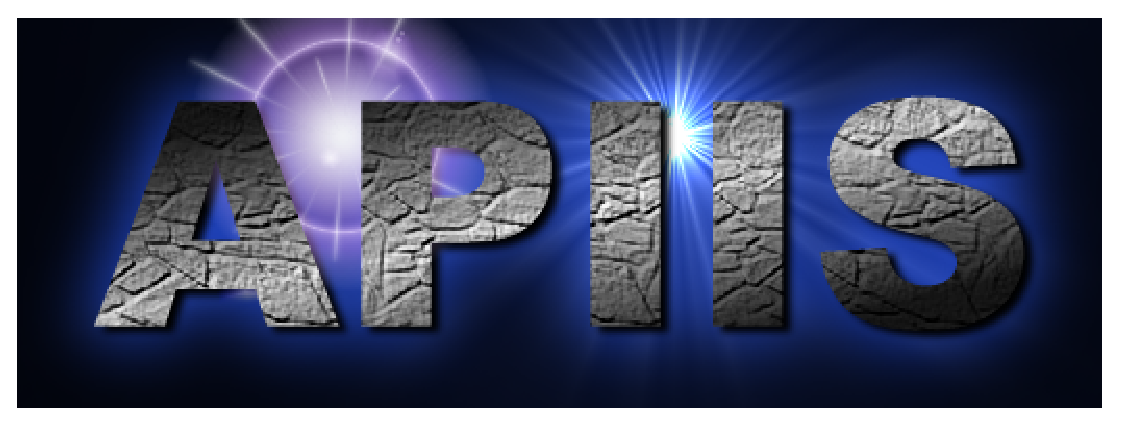
\includegraphics[scale=.7,]{../implementer/apiis6.ps}

\vspace{2cm}
\begin{Huge}\textbf{APIIS Implementer Documentation}\end{Huge}
\vspace{1cm}

\begin{Large}\textbf{written by}
\vspace{1cm}

\textbf{Eildert Groeneveld\\
           Zhivko Duchev\\
           Marek Imialek\\
           Helmut Lichtenberg\\
           Detlef Schulze\\
           Ulf M�ller \\
	        Ralf Fischer\\}\end{Large}
            \vspace{2cm}
\begin{large}\textbf{Mariensee,
                     September 2005}\end{large}
           \end{center}
                                                 %%\maketitle

      \newenvironment{lyxlist}[1]
        {\begin{list}{}
             {\settowidth{\labelwidth}{#1}
             \setlength{\leftmargin}{\labelwidth}
\addtolength{\leftmargin}{\labelsep}
\renewcommand{\makelabel}[1]{##1\hfil}}}
  {\end{list}}

\newcommand{\lyxrightaddress}[1]{
\par
{\raggedleft
\begin{tabular}{l}\ignorespaces
                                                                                                                                                                                                #1
                                                                                                                                                                                                   \end{tabular}
                                                                                                                                                                                                \vspace{1.4em}
                                                                                                                                                                                                       \par}
                                                                                                                                                                                                }



\tableofcontents
\chapter{Introduction}
In APIIS we define three groups of people working with the system. These
are:
\begin{description}
   \item[developers]the guys (and may be gals) developing the routines
   usually hidden from those people implementing a system
   \item[implementors]people who use the tools box to setup a running
   system, which pertains to a particular set of conditions. This may be
   the cattle population in one country
   \item[users]these are the people who in the end use the system
\end{description}
Clearly, we may sometime find persons who are both implementors and users. 

The developer's documentation covers all software  that is hidden from the
implementors. This means we are talking about the deep and sometimes dark
vaults and sometimes even dungeons of APIIS.

You may be surprised by the section "Undocumented subroutines". Currently,
   the meta layer of APIIS is being rewritten to an object oriented mode. 
   In this process, each routine that is handled will get its own
   documentation section in the Perl code. The subroutines listed here are
   of the non OO kind and will therefore have to converted/replaced by the
   developers. Thus, this chapter serves more like a reminder for them to
   get its length towards zero.

\chapter{Fixed APIIS Structure}

This chapter describes that part of the database structure which is
the same in all APIIS database.


\section{TRANSFER}


\section{CODES}


\section{UNIT, NAMING, ADDRESS}

These three tables cosntitute one block which administers all units,
persons and addresses in the database. As such it should be quite
generic and should be used, largely unchanged in every database.


\subsection{ADDRESS}

This table holds the individual physical addresses, one entry for
each. The primary key is the sequence DB\_ADDRESS


\subsection{NAMING}

Here we store all individual persons and organization which are part
of the system. Many people can have the same address, that is why
in a normalized way this has been split into ADDRESS and NAMING. The
primary key is the DB\_NAME which is a sequence.


\subsection{UNIT}

EXT\_ID is the external identification used in the outside world.
This may be the number or code {}``1'' for the veterinarians. Then
EXT\_UNIT would be {}``VET''. If we would merge veterinarians from
Bavaria and Saxony in one system, and the vets were numbered within
each state beginning with {}``1'', the EXT\_UNIT would be {}``VET-SAX''
and {}``VET-BAV''. In this way the old numbering systems can continue
to be used (which is actually the motivation for the EXT\_UNIT/EXT\_ID
setup. Thus, EXT\_UNIT has to be defined such that the EXT\_IDs being
used are made unique.

One other objective is the possibility to reuse external numbers.
Assume that the head veterinarian with EXT\_ID=''1'' retires and
is replaced by his successor. This person should again get the EXT\_ID=''1''.
Then, the same as in TRANSFER, the old EXT\_ID gets closed (CLOSING\_DT
is set) and a new record with the EXT\_=ID=''1'' is created.

The unique index is EXT\_UNIT||EXT\_ID where CLOSING\_DT is NULL.
This means that we are allowing one {}``open'' channel for the combination
of external unit and external identification.


\subsection{Navigation}

Access to ADDRESS and NAMING is straight forward. Let us assume a
new address is to be entered. The following steps are performed:

\begin{enumerate}
\item verify that the address to be entered does not already exist. This
can be done by search the table ADDRESS on any fields with a LIKE
expression.
\item enter a new address. The primary key is simply the sequence DB\_ADDRESS.
Note that EXT\_ADDRESS is just a plain column which may be used for
locating a record in an interactive manner. Notice that COUNTRY needs
to be defined in CODES (Foreign Key).
\end{enumerate}
It is the sole responsibility of the user to ensure that no duplicate
addresses are entered. While this may sound dangerous it is actually
the only logical way. If an address is entered twice there is really
no harm done as this and the other may be used together as DB\_ADRESS
will be used to link the address to people.

NAMING is delt with in a similar manner. The insertion process is
identical to ADDRESS:

\begin{enumerate}
\item verify that the person/organization to be entered does not already
exist by searching on any of the fields interactively.
\item insert the new person/organization. The primary key DB\_NAMING will
automatically come from a the sequence seq\_naming\_\_db\_nam. Notice
that LANGUAGE needs to be defined in CODES (Foreign Key).
\end{enumerate}
UNIT has a somewhat different position in this triplet. It defines
the telefonnumbers, fax, e-mail belonging to a person or organization
for a given role. To create a new external ID, let us say the second
veterinarian, we would do the following:

\begin{enumerate}
\item type EXT\_UNIT='VET' and EXT\_ID='2' into unit

\begin{enumerate}
\item locate the address of this person in ADDRESS (remember DB\_ADDRESS)
\item locate the person in NAMING (remember DB\_NAMING)
\end{enumerate}
\item insert record in UNIT with all data using DB\_ADDRESS and DB\_NAMING,
DB\_UNIT is derived from the sequence, OPENING\_DT is set to the current
date while CLOSING\_DT is NULL.
\end{enumerate}
Thus far, no statemens have been made as to the status of DB\_UNIT.
While in ADDRESS and NAMING the corresponding DB\_ columns function
as primary keys, this is not the case here. Thus, if the user choses
to create another {}``input channel'' for a different EXT\_UNIT/EXT\_ID
with the same DB\_UNIT nothing will prevent her from doing this. What
needs to be considered is however that a select on DB\_UNIT will then
return two records instead of one.

%%%%%%%%%%%%%%%%%%%%%%%%%%%%%% Textclass specific LaTeX commands.
 \newenvironment{lyxcode}
    {\begin{list}{}{
                           \setlength{\rightmargin}{\leftmargin}
                                \setlength{\listparindent}{0pt}% needed for
                                   AMS classes
                                        \raggedright
                                             \setlength{\itemsep}{0pt}
                                     \setlength{\parsep}{0pt}
                                          \normalfont\ttfamily}%
                                                 \item[]}
                                                    {\end{list}}

\chapter{The business and modify rules}


\section{The business rules}

The currently implemented business rules are shown in table \ref{tab:business rules}
on page \pageref{tab:business rules}.

\begin{table}[htbp]

\caption{Implemented Business Rules\label{tab:business rules}\index{business rules!Range}\index{business rules!List}\index{business rules!IsANumber}\index{business rules!NoNumber}\index{business rules!IsAFloat}\index{business rules!Unique}\index{business rules!ForeignKey}\index{business rules!DateDiff}\index{business rules!LastAction}\index{business rules!IsEqual}\index{business rules!ReservedStrings}}

\begin{center}{\small \vspace*{4mm}}\begin{sideways}
\begin{tabular}{|l|p{100mm}|p{50mm}|}
\hline 
\textbf{\small Method}&
\textbf{\small Description}&
\textbf{\small Example}\tabularnewline
\hline
\hline 
{\small Range}&
{\small value has to be within given range}&
{\small {}``Range 10 33''}\tabularnewline
\hline
{\small List}&
{\small only values from this list are allowed}&
{\small {}``List LR LW PI DU''}\tabularnewline
\hline
{\small NotNull}&
{\small has to have a value}&
{\small {}``NotNull''}\tabularnewline
\hline
{\small IsANumber}&
{\small only a number is accepted (5, -.37, +5.3e-3)}&
{}``IsANumber''\tabularnewline
\hline
{\small NoNumber}&
value must not contain any number &
{}``NoNumber''\tabularnewline
\hline
{\small IsAFloat}&
{\small value must be a floating point number (+4.3, .27, -0.5)}&
{}``IsAFloat''\tabularnewline
\hline
{\small Unique}&
{\small the value is a unique key in the current table}&
{\small {}``Unique''}\tabularnewline
\hline
{\small ForeignKey}&
{\small value has to have an entry in the specified table and column,
possibly with some additional conditions}&
{\small \mbox{{}``ForeignKey animal db\_animal'',}}{\small \par}

{\small ''ForeignKey v\_animal db\_animal ext\_sex=1 ext\_breed=DL''}\tabularnewline
\hline
{\small DateDiff}&
{\small the difference between the content of farrowing date and current
columns of the current record must be with the given range}{\small \par}

{\small DateDiff takes the current value of the record and computes
the difference to date given in the first parameter (compare\_date).
If the difference (in days) between the cure and compare\_date is
in the range given by min\_diff and max\_diff the rule is passed successfully. }{\small \par}

{\small compare\_date can either be a fixed format date like Mar-22-2001,
a column of the current record or a date in a database table/column
with the (hardcoded) db\_animal value of the current record. The syntax
for this format is 'tablename=>columname'. If no compare date comes
from the database the check is also successfully. }&
{\small \mbox{{}``DateDiff farrow\_dt 20 56'',}}{\small \par}

{\small \mbox{{}``DateDiff Mar-22-2001 50 90'',}}{\small \par}

{\small \mbox{{}``DateDiff animal=>birth\_dt 1 65''}}\tabularnewline
\hline
{\small LastAction}&
{\small LastAction is a conditional DateDiff depending on the value
of the last action. For each element of this last action list an allowed
range (in days) has to be specified.}{\small \par}

{\small If last action was SEL{[}ECTION{]} the range is 20 100, if
it was AI the range is 18 30}&
{\small {}``LastAction SEL 30 100 AI 18 30 LITTER 10 34''}\tabularnewline
\hline
IsEqual&
This example is placed in the CHECK attached to column db\_sire e.g.
in service and tests if the animal ID given is indeed a male. Thus,
the second parameter (i.e. \$data\_column) takes its value from the
current column Notice that the constant is specified as external code.&
IsEqual ( animal db\_animal db\_sex 'M'); \tabularnewline
\hline
ReservedStrings&
{\small ReservedStrings checks if the passed \$date contains one of
the reserved strings which are defined in pdblrc.}&
{\small {}``ReservedStrings''}\tabularnewline
\hline
\end{tabular}
\end{sideways}\end{center}
\end{table}



\section{The Modify Rules}

Sometimes it is necessary to modify the incoming value before it is
fed to the business rules. These modify methods are: \textbackslash{}par\textbackslash{}vspace\{4mm\}

\begin{center}\label{encode}\begin{tabular}{|l|p{80mm}|l|}
\hline 
\textbf{Method}&
\textbf{Description}&
\textbf{Example}\tabularnewline
\hline
\hline 
UpperCase&
converts all passed date into uppercase letters&
{}``UpperCase''\tabularnewline
\hline 
LowerCase&
converts all passed date into lowercase letters&
{}``LowerCase''\tabularnewline
\hline 
ConvertBool&
accepts YyJjNn and converts it to the appropriate boolean expression
(true/false)&
{}``ConvertBool''\tabularnewline
\hline 
CommaToDot&
translates all commas , into dots . (mainly used for numerical date)&
{}``CommaToDot''\tabularnewline
\hline 
DotToColon&
translates all dots . into colons : (useful for fast typing of date/time
values (16.34.00 => 16:34:00&
{}``DotToColon''\tabularnewline
\hline 
SetNow&
sets the value to the current time&
{}``SetNow''\tabularnewline
\hline
SetUser&
sets the value to the user who is running this job&
{}``SetUser''\tabularnewline
\hline
\end{tabular}\end{center}


\section{Layering\index{Layering} of Business Rules}

As described above, all business rules are specified as properties
of the the columns nd are thus part of their definition. This results
in one set of rules applied to any database modifications. However,
there may be circumstances that one set of rules is not sufficient
to describe all data coming into the database. For instance, the database
may contain data from the nucleus level of a breeding program and
also data from the production level. Clearly, business rules may be
different for the two types of data. To accommodate this situation
APIIS has implemented sets or layers of business rules. The philosophy
behind this is, that data streams can be subdivided into distinct
classes of data which have their own set of rules. Examples are (as
mentioned above) nucleus versus production level. Others could be
fat breeds versus less fat (like Meishan vs Landrace).

Operationally, business rules layers are defined as additional CHECK
in the model file. They are written as CHECK1\index{CHECK1} for a
layer 1, CHECK2\index{CHECK2} for a layer 2 etc. An example is given
in table \ref{cap:check levels}. The column db\_sex requires is a
foreign key in CODES and must not be NULL in the base (default) level
as indicated by the the key CHECK. If no check\_level (chk\_lvl\index{chk\_lvl})
is specified those given by CHECK apply. Its explicit chk\_lvl is
0. On the other hand the chk\_lvl=1 has only the foreign key requirement.
Thus, at this level NULL values for sex will be allowed. 

The procedure for specifying and using layered business rules is as
follows:

\begin{enumerate}
\item determine the number of layers of business rules required in your
set of data streams. This means that you should group together classes
of records that have similar requirements regarding the business rules.
Examples are: nucleus population, multiplier level, production level.
Or small breeds version large breeds. Also, combinations are possible.
These levels should get entries for documentation purposes in CODES\index{CODES}
under class CK\_LVL.
\item write the basic set of rules in the model file using the key CHECK.
The set of rules specified here will be the basic level that is used.
Thus, it will be used if either CHK\_LVL is set to 0 or not set at
all. Then specify for each check level a corresponding CHECKn rule.
Thus, if you decided to have three check levels you will have CHECK,
CHECK1 and CHECK2 in your model file. While CHECK should be specified
as the base set of rules, the other CHECKs are specified only if the
base CHECK is not applicable. Thus, whenever a CHECK key exists for
a given column corresponding the chk\_lvl specified it will replace
the base CHECK. Then this set of business rules will be executed.
As can be seen in table \ref{cap:check levels} only for column db\_sex
are the business rules modified in level 1. In db\_breed only the
base is specified, thus for all other chk\_lvl that may be specified
only the base set of checks are performed.
\item as has been said above, prior to enforcing the business rules the
programmer needs to specify which level she/he wants to fire. This
is typically done in the load object by calling the routine: \$pdbl->Model->set\_checklevel\index{set\_checklevel}
(1); In this example it would be set to 1. If you specify a check
level that does not exists in the model file at least once the calling
program should stop.
\item With a number of possible check levels, the current level that was
used when the database content was modified (insert or update) needs
to be stored with the record in each table. This is done in the column
CHK\_LVL. This is read and used in the program check\_integrity\index{check\_integrity}
to fire the correct set of business rules.
\end{enumerate}
%
\begin{table}[htbp]

\caption{\label{cap:check levels}Specifying layers of business rules}

\begin{lyxcode}
{\scriptsize col002~=>~\{~DATA~=>~'',~}{\scriptsize \par}

~{\scriptsize ~~~~~~~~~~~DB\_COLUMN~~~=>~'db\_sex',~}{\scriptsize \par}

~{\scriptsize ~~~~~~~~~~~DATATYPE~~~~=>~'BIGINT',~}{\scriptsize \par}

~{\scriptsize ~~~~~~~~~~~LENGTH~~~~~~=>~'1',~}{\scriptsize \par}

~{\scriptsize ~~~~~~~~~~~DESCRIPTION~=>~'sex',~}{\scriptsize \par}

~{\scriptsize ~~~~~~~~~~~DEFAULT~~~~~=>~'',~}{\scriptsize \par}

~{\scriptsize ~~~~~~~~~~~CHECK~~~~~~~=>~{[}'ForeignKey~codes~db\_code',~'NotNull'{]},~}{\scriptsize \par}

~{\scriptsize ~~~~~~~~~~~CHECK1~~~~~~=>~{[}'ForeignKey~codes~db\_code'{]},~}{\scriptsize \par}

~{\scriptsize ~~~~~~~~~~~MODIFY~~~~~~=>~{[}{]},~}{\scriptsize \par}

~{\scriptsize ~~~~~~~~~~~ERROR~~~~~~~=>~{[}{]},~}{\scriptsize \par}

{\scriptsize \},~}{\scriptsize \par}

{\scriptsize col003~=>~\{~~~~~~~~~~}{\scriptsize \par}

~{\scriptsize ~~~~~~~~~~~DATA~~~~~~~~=>~'',~~~~~~~~~~}{\scriptsize \par}

~{\scriptsize ~~~~~~~~~~~DB\_COLUMN~~~=>~'db\_breed',~~~~~~~~~~}{\scriptsize \par}

~{\scriptsize ~~~~~~~~~~~DATATYPE~~~~=>~'BIGINT',~~~~~~~~~~}{\scriptsize \par}

~{\scriptsize ~~~~~~~~~~~LENGTH~~~~~~=>~'2',~~~~~~~~~~}{\scriptsize \par}

~{\scriptsize ~~~~~~~~~~~DESCRIPTION~=>~'breed',~~~~~~~~~~}{\scriptsize \par}

~{\scriptsize ~~~~~~~~~~~DEFAULT~~~~~=>~'',~~~~~~~~~~}{\scriptsize \par}

~{\scriptsize ~~~~~~~~~~~CHECK~~~~~~~=>~{[}'NotNull',~'ForeignKey~codes~db\_code'{]},~~~~~~~~~~}{\scriptsize \par}

~{\scriptsize ~~~~~~~~~~~MODIFY~~~~~~=>~{[}{]},~~~~~~~~~~}{\scriptsize \par}

~{\scriptsize ~~~~~~~~~~~ERROR~~~~~~~=>~{[}{]},~~~}{\scriptsize \par}

{\scriptsize \},~}\end{lyxcode}

\end{table}




\chapter{Writing Load Objects}

Load objects carry out the database manipulation originating from
one record from a data stream. A load object groups together all database
manipulations required for a separate selfcontained record from a
data stream. As such all the database manipulations either fail (rollback\index{rollback})
or succeed (commit\index{commit}). It is important to notice that
a LO is completely self contained. Its only connection to the outside
world is the model file (which is implicit) and the LO\_keys. These
are in fact the fields that constitute the data stream under consideration.
Being selfcontained and parameterized from the outside the load object
can either be called from a batch\index{Datastream!batch} program
or an interactive GUI program\index{Datastream!GUI}. 

In case some of the business rules are violated, the transaction is
aborted and rolled back (in case some database modifications were
already done). The errors are returned in a data structure of its
own and leave it processing to the calling program. In batch processing
the errors are written into the appropriate database tables, GUIs
usually have to shown the errors in the form immediately.

One function of the load objects is the relate error to the fields
that held the data. These are usually the keys in the LO\_keys. However,
for the reference fileds of the model file, e.g. db\_animal, db\_code, db\_address, this may
become quite involved. Consider the database column db\_animal. This
is the internal animal number after translation from the outside external
identifications to the internal. In particular, db\_animal is a function
of db\_unit which in turn is derived from CLASS / EXT\_code. This
means that db\_animal depends on three external identifications. In
this case all three may get marked as being the culprit.


\section{The pseudo SQL code, general syntax}

The connection between the source data fields and the checking in
the business rules layer (well hidden in the routine meta\_db which
is called in the load object) is derived from the pseudo SQL code
used for database modifications in the LO. Up to now select, insert
and update statements could be used with these pseudo SQL syntax.
The example in table \ref{pseudoSQL} implies an insert of a record
in table MYTABLE with the columns animal\_nr, weight, and weigh\_dt.
The values for the three columns are taken from the perl variables
\$animal\_nr, \$weight, and \$measure\_dt. It is a requirement that
these source variables are part of the data input hash LO\_keys to
the LO. Typically, they will come from the outside world (outside
the LO) either from INSPOOL records for batch programs or the GUI
fields for GUI programs. These keys are also used in the error hash
(for description see \ref{errorhash})to collect any errors that may
occur during execution of the business rules.

Sometimes data elements are also generated in the LO itself. This
may be the case in the processing of birth records in pigs, where
individual piglet identifications are generated on the basis of number
of piglets born (see LO\_DS02 for an example). Here, we would have
additional source variables that are not part of the input hash LO\_hash.
If this variable is to be used in the pseudo SQL code and must be
added to the hash LO\_keys. Only then can the error processing code
the 'culprit' i.e. the source variable responsible for the error (should
there be an error).

%
\begin{table}[htbp]

\caption{\label{pseudoSQL}the pseudo SQL in the load objects}

\begin{lyxcode}
\$pseudo\_sql{[}0{]}=~(

~~~~~~~'INSERT~into~MYTABLE~(

~~~~~~~~~~~~~~~~animal\_nr,~~weight,~~~weigh\_dt

~~~~~~~)VALUES~(

~~~~~~~~~~~~~~~\$animal\_nr,~\$weight,~\$measure\_dt)'

);\end{lyxcode}

\end{table}


In the following we will discuss the load object LO\_DS01.pm\index{Load Object!LO\_DS01.pm}
with the matching DS01.pm\index{Datastream!DS01.pm} as it is used
in batch processing.


\section{The pseudo SQL code with ENCODING}

The APIIS design feature to disconnect the outside coding from it
internal representation, while providing flexibility for future changes,
does require additional action during database access. This action
is the required translation of any external coding into internal codes
used throughout the database. There are two ways to deal with this
translation. Firstly, in the LO the programmer can retrieve the internal
codes by using standard DBI accesses to the database and then use
the retrieved internal codes in the pseudo SQL code. While it provides
flexibility, it does require error handling which can be avoided by
using the second mechanism.

Here, when the model file contains in the CONSTRAINTS section of a table the expression REF\_COL:column\_name1 then only the external codes must be used and not internal ones. The situation is the same when we have in the CHECK section of a column ForeignKey rule that leads in the end to reference column. If this is used, the BR layer
must only contain external codes and not internal ones. There is one important exception from this rule: when we want to insert a new animal in transfer, new code in table codes, i.e. new internal identificator, we have to supply the internal number as shown in the following example:
\begin{verbatim}
my $db_animal2=$apiis->DataBase->seq_next_val('seq_transfer__db_animal');
	 $data_hash{db_animal2} = $db_animal2;

         # generate new piglet numbers:
         $data_hash{piglet} = $data_hash{dam_hb_nr} . '|' . $notch;

         $pseudo_sql_2[0] =
            'INSERT INTO transfer (
                    db_animal,
                    ext_animal,
                    db_unit,
                    opening_dt,
                    entry_dt,
                    db_entry_action
            ) VALUES (
                    $db_animal2,
                    $piglet ["start_notch_no, born_alive_no"] ,
                    concat( "society|sex", $dam_society."|2" ),
                    $today[],
                    $today[],
                    "birth"
	    )' ;
\end{verbatim} 


\section{The error hash\label{errorhash}}

The generell structure of the error hash is described in the library
Apiis::Errors. The predefined keywords and structure is shown in Table
\ref{cap:Structure-of-error}.

%
\begin{table}[htbp]

\caption{Structure of error hash\label{cap:Structure-of-error}}

\begin{lyxcode}
{\footnotesize my~@type\_values~=~qw/~DATA~DB~OS~PARSE~CODE~PARAM~CONFIG~UNKNOWN~/;~}{\footnotesize \par}

{\footnotesize \#~Error~types:~}{\footnotesize \par}

{\footnotesize \#~DATA~the~passed~data~is~not~ok~(usually~in~CheckRules)~~~~~~~~~~~~~~~~}{\footnotesize \par}

{\footnotesize \#~DB~errors~from~the~database~(e.g.~unique~index~violation)~}{\footnotesize \par}

{\footnotesize \#~OS~errors~from~the~operation~system~(e.g.~full~hard~disk)~}{\footnotesize \par}

{\footnotesize \#~PARSE~errors~in~ParsePseudoSQL~with~parsing~pseudo~SQL~code~}{\footnotesize \par}

{\footnotesize \#~CODE~programming~errors,~e.g.~from~applications~like~load~objects~}{\footnotesize \par}

{\footnotesize \#~PARAM~passed~parameter~is~wrong~or~missing~}{\footnotesize \par}

{\footnotesize \#~CONFIG~one~of~the~configuration~files~is~wrong~or~has~missing~entries~}{\footnotesize \par}

{\footnotesize \#~UNKNOWN~is~unknown~:\textasciicircum{})}{\footnotesize \par}

{\footnotesize my~@severity\_values~=~qw/~FATAL~NON-FATAL~/;~}{\footnotesize \par}

{\footnotesize my~@action\_values~=~qw/~INSERT~UPDATE~DELETE~SELECT~DECODE~ENCODE~UNKNOWN~/;}{\footnotesize \par}

{\footnotesize \#~structure~of~error~messages:}{\footnotesize \par}

{\footnotesize my~\%struct;~tie~\%struct,~'Tie::IxHash';}{\footnotesize \par}

{\footnotesize \%struct~=~(~type~=>~undef,~\#~predefined~values~above~}{\footnotesize \par}

~{\footnotesize ~~~~~~~severity~=>~undef,~\#~predefined~values~above~}{\footnotesize \par}

~{\footnotesize ~~~~~~~~~action~=>~undef,~\#~predefined~values~above}{\footnotesize \par}

~{\footnotesize ~~~~~~~~~~~from~=>~undef,~\#~location~where~this~error~comes~from~(e.g.~sub,~rule)~}{\footnotesize \par}

~{\footnotesize ~~~~~~record\_id~=>~undef,~\#~id~of~this~record,~e.g.~record\_seq~from~inspool}{\footnotesize \par}

~{\footnotesize ~~~~~~~~~~~unit~=>~undef,~\#~unit~that~provides~this~data}{\footnotesize \par}

~{\footnotesize ~~~~~~~db\_table~=>~undef,~\#~database~table~concerned}{\footnotesize \par}

~{\footnotesize ~~~~~~db\_column~=>~undef,~\#~database~column~concerned}{\footnotesize \par}

~{\footnotesize ~~~~~~~~~~~data~=>~undef,~\#~just~handled~incorrect~data}{\footnotesize \par}

~{\footnotesize ~~~~~~~ext\_cols~=>~undef,~\#~involved~external~columns~(array)}{\footnotesize \par}

~{\footnotesize ~~~~~~~~~~~~~ds~=>~undef,~\#~data~stream~name}{\footnotesize \par}

~{\footnotesize ~~~~~~~err\_code~=>~undef,~\#~coded~error~message}{\footnotesize \par}

~{\footnotesize ~~~~~~msg\_short~=>~undef,~\#~main~error~message~for~end~users}{\footnotesize \par}

~{\footnotesize ~~~~~~~msg\_long~=>~undef,~\#~detailed~error~message}{\footnotesize \par}

~{\footnotesize ~~~~~~~~~~misc1~=>~undef,~\#~user~defined~scalar}{\footnotesize \par}

~{\footnotesize ~~~~~~~~~~misc2~=>~undef,~\#~user~defined~scalar}{\footnotesize \par}

~{\footnotesize ~~~~~~misc\_arr1~=>~undef,~\#~user~defined~array}{\footnotesize \par}

~{\footnotesize ~~~~~~misc\_arr2~=>~undef,~\#~user~defined~array}{\footnotesize \par}

~{\footnotesize ~~~~~~~~~);~}\end{lyxcode}

\end{table}



\section{An example: The Load Object LO\_DS01\index{Load Object!LO\_DS01}}

The simple load object LD\_DS01 performs the database actions related
with a new insemination record. In this example it needs to do:

\begin{enumerate}
\item Insert new record into SERVICE\index{table!SERVICE} 
\item Update last action (la\_rep) in ANIMAL\index{table!ANIMAL}
\end{enumerate}
%
\begin{table}[htbp]

\caption{\texttt{\small LO\_DS01.pm\label{tab:LO-DS01.pm}\index{Load Object!LO\_DS01.pm}}}

\texttt{\small ~ 1 \#\#\#\#\#\#\#\#\#\#\#\#\#\#\#\#\#\#\#\#\#\#\#\#\#\#\#\#\#\#\#\#\#\#\#\#\#\#\#\#\#\#\#\#\#\#\#\#\#\#\#\#\#\#\#\#\#\#\#\#\#\#\#\#\#\#\#\#\#}{\small \par}

\texttt{\small ~ 2 \# \$Id: actual\_docu.lyx,v 1.37 2003/12/15 13:54:40
eg Exp \$}{\small \par}

\texttt{\small ~ 3 \# This is the Load Object for a new insemination
record.}{\small \par}

\texttt{\small ~ 4 \# It is responsible to:}{\small \par}

\texttt{\small ~ 5 \#~~~~~~~~~~ 1. Insert new record into
SERVICE}{\small \par}

\texttt{\small ~ 6 \#~~~~~~~~~~ 2. Update last action (la\_rep)
in ANIMAL}{\small \par}

\texttt{\small ~ 7 \#\#\#\#\#\#\#\#\#\#\#\#\#\#\#\#\#\#\#\#\#\#\#\#\#\#\#\#\#\#\#\#\#\#\#\#\#\#\#\#\#\#\#\#\#\#\#\#\#\#\#\#\#\#\#\#\#\#\#\#\#\#\#\#\#\#\#\#\#}{\small \par}

\texttt{\small ~ 8 sub LO\_DS01 \{}{\small \par}

\texttt{\small ~ 9~~~ my \%data\_hash = \%\{ shift () \};}{\small \par}

\texttt{\small ~10~~~ }{\small \par}

\texttt{\small ~11 }{\small \par}

\texttt{\small ~12~~~ \# These are the required LO\_keys for DS01.pm:}{\small \par}

\texttt{\small ~13~~~ my @LO\_keys = qw( dam\_hb\_nr dam\_society
dam\_breed sire\_hb\_nr}{\small \par}

\texttt{\small ~14~~~~~ sire\_society sire\_breed service\_dt
);}{\small \par}

\texttt{\small ~15 }{\small \par}

\texttt{\small ~16~~~ \# some basic checks:}{\small \par}

\texttt{\small ~17~~~ my ( \$err\_status, \$err\_ref ) = CheckLO(
\textbackslash{}\%data\_hash, \textbackslash{}@LO\_keys );}{\small \par}

\texttt{\small ~18~~~ return ( \$err\_status, \$err\_ref ) if
\$err\_status;}{\small \par}

\texttt{\small ~19 }{\small \par}

\texttt{\small ~20~~~ my @pseudo\_sql;}{\small \par}

\texttt{\small ~21~~~ \$pseudo\_sql{[}0{]} = (}{\small \par}

\texttt{\small ~22~~~~~~ 'INSERT into service (}{\small \par}

\texttt{\small ~23~~~~~~~~~~ db\_animal,}{\small \par}

\texttt{\small ~24~~~~~~~~~~ db\_sire,}{\small \par}

\texttt{\small ~25~~~~~~~~~~ service\_dt,}{\small \par}

\texttt{\small ~26~~~~~~~~~~ db\_service\_typ}{\small \par}

\texttt{\small ~27~~~~~~ ) VALUES (}{\small \par}

\texttt{\small ~28~~~~~~~~~~ concat( \char`\"{}society|sex\char`\"{},
\$dam\_society.\char`\"{}|2\char`\"{}, \$dam\_hb\_nr ),}{\small \par}

\texttt{\small ~29~~~~~~~~~~ concat( \char`\"{}society|sex\char`\"{},
\$sire\_society.\char`\"{}|1\char`\"{}, \$sire\_hb\_nr ),}{\small \par}

\texttt{\small ~30~~~~~~~~~~ \$service\_dt,}{\small \par}

\texttt{\small ~31~~~~~~~~~~ \char`\"{}insem\char`\"{})'}{\small \par}

\texttt{\small ~32~~~ );}{\small \par}

\texttt{\small ~33 }{\small \par}

\texttt{\small ~34~~~ \$pseudo\_sql{[}1{]} = (}{\small \par}

\texttt{\small ~35~~~~~~ 'UPDATE animal SET}{\small \par}

\texttt{\small ~36~~~~~~~~ la\_rep~~~ = \char`\"{}SERVICE\char`\"{},}{\small \par}

\texttt{\small ~37~~~~~~~~ la\_rep\_dt = \$service\_dt}{\small \par}

\texttt{\small ~38~~~~~~~~ where db\_animal = concat( \char`\"{}society|sex\char`\"{},
\$dam\_society.\char`\"{}|2\char`\"{}, \$dam\_hb\_nr )'}{\small \par}

\texttt{\small ~39~~~ );}{\small \par}

\texttt{\small ~40 }{\small \par}

\texttt{\small ~41~~~ \$apiis->DataBase->dbh->commit;~~~ \# clean start of transaction}{\small \par}

\texttt{\small ~42~~~ \$hash\_ref = meta\_db( \textbackslash{}@pseudo\_sql,
\textbackslash{}\%data\_hash );}{\small \par}

\texttt{\small ~43~~~ \$hash\_ref->\{err\_status\} ? \$apiis->DataBase->dbh->rollback
: \$apiis->DataBase->dbh->commit;}{\small \par}

\texttt{\small ~44~~~ return ( \$hash\_ref->\{err\_status\}, \$hash\_ref->\{err\_ref\}
);}{\small \par}

\texttt{\small ~45 \}}{\small \par}

\texttt{\small ~46 }{\small \par}

\texttt{\small ~47 1;}
\end{table}


\begin{lyxlist}{00.00.0000}
\item [lines~9~--~10:]The input parameters are passed from DS01 (or
from a GUI\_DS01) (via subroutine \texttt{\scriptsize Process\_LO\_Batch}).
Some data streams need the reporting unit for their processing, others
(like LO\_DS01) can simply ignore it.
\item [lines~13~--~14:]This defines the names of the external data fields
which have to be used by any program that sends data to this load
object. (Actually, LO\_keys is a sufficient set of information to
run the Load Object. It needs to be derived directly from the data
streams that should have been described before.)
\item [lines~17~--~18:]CheckLO test the accordance of LO\_keys with
the keys of the \%data\_hash.
\item [lines~20~--~39:]A SQL-like description language is used to pass
the parameters to the subsequent processing. This PseudoSQL is described
in section .
\item [line~41:]A commit\index{database!commit} to the database is executed
to start this transaction with a well defined status.
\item [line~42:]All needed parameters (PseudoSQL and the data hash) are
passed to the subroutine meta\_db() which prepares and executes the
database actions.
\item [line~43:]Depending of the return status of meta\_db() the transaction
is committed or rolled back\index{database!rollback}.
\item [line~44:]The load object returns either success (\$err\_status
= 0) or an error status $>$ 0 and the accompanied error messages.
\end{lyxlist}

\subsection{Passing parameters with PseudoSQL\label{section:PseudoSQL}\index{Load Object!PseudoSQL}}

To pass the parameters to the subroutine meta\_db() for database transactions
it was decided to choose a SQL-like syntax. This description language
is parsed later to extract the important variables and data. These
are the rules for parsing PseudoSQL: 

\begin{itemize}
\item The Pseudo-SQL-Statements must be surrounded by \textbf{single} quotation
marks. No substitution of the Perl variables should take place. PseudoSQL
is only an artificial language to pass the parameters. Strings inside
these statements must be framed by \textbf{double} quotation marks.
\\
Example: \texttt{\small \$pseudo\_sql{[}0{]} = 'INSERT into litter
( db\_animal, delivery\_dt, comment ) VALUES ( \$dam\_hb\_nr, \$delivery\_dt,
\char`\"{}this is a comment\char`\"{} );} 
\item To concatenate values you can use the key word 'concat'. The single
elements of this concatenation must be separated by commas. Fixed
strings and variables can be mixed. The Perl concatenation operator
. can also be used. \\
Example: \texttt{\small concat( \char`\"{}society|sex\char`\"{}, \$dam\_society
. \char`\"{}|2\char`\"{}, \$dam\_hb\_nr )}{\small \par}
\item Variables, whose names do not point to an external field of the incoming
data stream can be assigned external names in brackets. The names
in brackets \textbf{must} be surrounded by double quotation marks
in total, not every single element. \\
Examples: \texttt{\small \$piglet{[}\char`\"{}start\_notch\_no, born\_alive\_no\char`\"{}{]}
concat(\char`\"{}society|sex\char`\"{}, \$dam\_society .\char`\"{}|2\char`\"{},
\$piglet{[}\char`\"{}start\_notch\_no, born\_alive\_no\char`\"{}{]})} 
\item Do you use a variable that does not point to any external field you
have to supply this variable with empty brackets. \\
Example: \texttt{\small \$today{[}{]}}{\small \par}
\item All variables, that you use in the Pseudo-SQL-Statements have to appear
as a key (without the dollar character \$) in the \%data\_hash which
you pass to meta\_db(). Usually this will be the (already existing)
field names of the incoming data. You have to add variables which
newly appear in the load object like \$piglet, \$today, \$now or also
the separately passed external unit \$ext\_unit. Just have a look
into LO\_DS02.pm for some examples.
\end{itemize}

\section{Calling a Load Object and some other issues}

As stated above a load object needs to get its input values (i.e.
the data elements defined for that particular data stream) from a
calling program. There are two modes how this can be done: input comes
from a batch program, i.e. data are read from a file or data are entered
via a GUI\index{GUI} program. A description of the former is to be
found in the inspool section of this document. GUI programs on the
other hand can be created automatically by the program mkLOform which
may be called as: \texttt{mkLOform LO\_{*} '\$PDBL\_LOCAL/model/apiis.model'}
\index{mkLOform}. As output it creates for each matching load object
one GUI program. What happens is that mkLOform picks up the LO\_key\index{key}
line from the load object which holds all elements defined for the
data stream. Then it creates for each of these elements one GUI field.
The GUI program can be run right away allowing the user to enter data
into the fields and sending them to the load object by pressing the
insert button. From there on the load object takes over doing all
the database interactions defined under the control of the business
rules.

The fields in the GUI program can be moved around the canvas using
the FormDesigner \index{FormDesigner}to suit the artistic and ergonomic
requirements of the user.

Sometimes data need to be derived from individual data. One example
is the individual recording of piglet weight at birth from which we
may want to derived the total number born, the sum of males and female
piglets and the total litter weight at birth (while this implies redundancy
we still may want to do it). To generate these sums in a Perl code
is very easy, thus doing this in the load object is a piece of cake.
However, there is the problem of not knowing in advance how many piglet
a litter has. One way of approaching this problem would be to have
one record for the sow and birthdate and the one for each piglet.
This has a number of problems: firstly, the complete set of information,
i.e. all the records pertaining to one litter constitute a transaction.
If we split this up into separate database activities, we cannot roll
the already entered data back should a later database action require
this. Secondly, one litter plus the piglet information are infact
a unit that the person entering the data would like to see as one
block. Thus, it would be desirable to have the GUI form start with
the block on the sow and then have one line for each piglet. Thus,
we would need to have enough space for a litter, 20 lines should be
ok. Then after the last piglet has been entered the complete form
content will be processed by the load object and do the necessary
accumulations on those variables that are not undef. The program mkLOform
\index{mkLOform} will then again generate the GUI program. Because
it places all fields below each other FormDesigner\index{FormDesigner}
will have to be used to arrange the fields in a more meaningful way.

This little paragraph reflect the progress made since the last one
was written. Because we are essentially lazy people Hartmut has meanwhile
rewritten mkLOform\index{mkLOfrm} into mkLOfForm\index{mkLOfForm} 
formatted forms from load objects) which produces GUI programs
on the basis of the LO\_Keys from the load objects that does multiple
fields per line. This is simply done by arranging the entries in the
LO\_Keys as is desired in the GUI program. An example is given in
table \ref{cap:Arrangement-of-keys}. The arrangement given will result
in a GUI program with 5 lines. The first would be one field with ext\_unit,
the second line would hold the three fields dam\_hb\_nr, dam\_society
and dam\_breed. The program is given in figure \ref{cap:GUI-program-automatically}.

%
\begin{table}[htbp]

\caption{\label{cap:Arrangement-of-keys}Arrangement of keys for the GUI program}

\begin{lyxcode}
~{\scriptsize ~~my~@LO\_keys~=~qw~(~}{\scriptsize \par}

~{\scriptsize ~~~~~~~~~~~~~~~~~~~~ext\_unit~~~~~~~~~~~~~~~~~~~~~~~}{\scriptsize \par}

~{\scriptsize ~~~~~~~~~~~~~~~~~~~~dam\_hb\_nr~~~~~dam\_society~~~~~dam\_breed}{\scriptsize \par}

~{\scriptsize ~~~~~~~~~~~~~~~~~~~~sire\_hb\_nr~~~~sire\_society~~~~sire\_breed}{\scriptsize \par}

~{\scriptsize ~~~~~~~~~~~~~~~~~~~~parity~~~~~~~~start\_notch\_no~~delivery\_dt~~~~~~~~}{\scriptsize \par}

~{\scriptsize ~~~~~~~~~~~~~~~~~~~~born\_alive\_no~weaned\_no~~~~~~~weaning\_dt~~~~~~~~~~~~~~~~~~}{\scriptsize \par}

~{\scriptsize ~~~~~~~~~~~~~~~~~~~);~}\end{lyxcode}

\end{table}


%
\begin{figure}[htbp]

\caption{\label{cap:GUI-program-automatically}GUI program automatically created
from LO\_DS02.pm}

%\begin{center}\includegraphics[%
  %  EG scale=0.4]{writing-LO/LO_DS02frm.png}
%  \end{center}
\end{figure}




\chapter{Initial Loading of Historic Data}

Very rarely, a new information system can be set up without any previouly
collected data. This implies the necessity to load all previously
collected data into the new database before the routine data flow
can start reaching the database. Historic data will typically be available
from a number of different and often independant source or oven organization.
As a consequence, many logical inconsistancies will be found in the
data once they are loaded into a target structure that defines a possibly
stringent set of business rules. As historic data may come in non
predictable way (many files, any format), a procedure was developed
which is as far as possible generic and thereby adaptable to any type
of animal data recording system. It therefore allows any number of
data files to be involved and furthermore, develops a strategy to
deal with the potentially large number of errors that will become
obvious once loaded into the business rule centered database.


\section{The General Procedure}

Once the structure of the database has been defined it has to be populated
with historic data, i.e. information already available in some computer
compatible form. As has been described above, all external codes or
identifications are translated into internal database codes to allow
for reuse of external codes should the meaning of them change at some
time. 

\begin{enumerate}
\item Operate on codes and external identification

\begin{enumerate}
\item Collect all temporary external codes
\item check external codes and determine their target code to go into the
database
\item determine illegal values and handle them
\item identify and handle duplicate identifications
\item create input channels for corrected external codes in the database.
The external codes can thus also be viewed as foreign keys which need
to be available in the database prior to load the data.
\end{enumerate}
\item Operate on data

\begin{enumerate}
\item load historic data using the channels created in the previous step
\item verify the loaded data against the business rules and flag records
with errors in the database
\end{enumerate}
\item Wrap up

\begin{enumerate}
\item rewrite the temporary external animal identification to the external
IDs reaching the database in routine data flow
\end{enumerate}
\end{enumerate}
Now we shall describe the steps in a little more detail.

\begin{enumerate}
\item Operate on codes and external identification


In this step only external codes and external identifications are
considered, leaving other data on animals like their measurement aside.
It is a step which basically collects, edits and loads Foreign Key
information into the database. From the programming perspective, this
process can be highly generic with little programming required by
the adaptor (once the generic code has been written).

\begin{enumerate}
\item {}``Collect all external codes'': In APIIS we have three groups
of external codes:

\begin{itemize}
\item animal identifications; this can be any combinations of data fields
that identify an animal uniquely in the historic data set. This is
not necessarily the external ID that may be used in later routine
data reporting. Its sole purpose is to identifiy individual animals
correctyl in the historic data sets. The definition of this temporary
external ID can be different from the external IDs used and reported
during routine data flow.
\item an address or partner identification
\item classical codes like the numeric representation of a breed or a code
for a certain abnormality
\end{itemize}
\item {}``check external codes'': like all data also identifications and
codes can be erroneous or inconsistant. As an example the breed {}``Pietrain''
may be coded in some files as {}``PI'' in others as {}``pi''.
Not only should the data made consistant but also a procedure must
exist to handle records that are identified as being incorrect. The
basic principles that we have followed is to provide for each external
code or identication the opportunity to translate it into a new target
value or as illegal by manual intervention. Then in the following
process (like loading of data) any occurence of the original value
will be replaced by its translated value.
\item {}``determine illegal values'': some identifications will be illegal.
For example, unknown sires may be codes as {}``~~~~~~'' or
as {}``999999''. These are not legal external identifications, and
should thus not be used to create a data channel. Also, if these IDs
come up later on in the loading process they should be skipped.
\item {}``duplicates'': The same ID must not be used for different animals.
This can happen when animal IDs are being reused after a number of
years. For some records we know that they should appear only once
for an animal: a field performance test may be an example. Here we
can test for multiple occurences. If duplicates are found then human
interaction is required to resolve the problem. 
\item {}``create input channnels'': Once all the target codes have been
established by manual human intervention, likewise duplicates and
undefined IDs have been dealt with, the external IDs get loaded into
the database. This populate the tables TRANSFER , CODES and UNIT.
\end{enumerate}
\item Operate on data


After the {}``foreign keys'' have been collected, edited and loaded
in the first block, now actual measurements have to be loaded into
the database. The translation tables edited manually in the first
step are also used here as filter.

\begin{enumerate}
\item {}``load historic data'': For each file containing historic data
a parameter file has to be written. This requires knowledge of the structure
of the data files and the database. The definition of the external
codes are identical to those in the first step. They are then passed
through the translation created by manual intervention. However, the
business rule layer is bypassed as time sequence dependant checks
cannot be made because data get processed in random order.
\item {}``Verify the loaded data'': Thus far all database modifications
have bypassed the business rule layer of the model file. The business
rule set can only be used if data come in correct time sequences which
clearly cannot be done when loading historic data. Thus, conflicts
with the business rules can be expected. Rows violating the business
rules will be flagged {}``dirty''. This allows a selection of correct
data during later database operation. Furthermore, {}``dirty'' records
can be cleaned up successively later on.
\end{enumerate}
\item Wrap up


In the previous step all historic data has been loaded, verified against
the business rules and flagged accordingly. Now the routine data flow
can start using the data stream model. But before this can be done,
the data channels may have to be translated from the temporary external
animal ID to the ID that comes in via the routine data streams. The
temporariy external IDs were created for the purpose of uniquely identifying
data records in the historic datasets. Thus, after loading, they have
served their purpose and may be modified. In the historic dataset,
initially there may have been duplicate IDs refering to different
animals. By adding the birth year they would have been made unique:
4711 in 1990 and in 1999 would have been identified as 4711$|$90 and
4711$|$99. The former animal will not be active any more while data
for the latter will still come into the system. However, it will be
identified in the data stream only as 4711. Thus, its external number
can be changed to 4711. Accordingly, incoming data to animal 4711
will find an open data channel and be translated to the correct internal
database number.

\end{enumerate}

\section{Description of the loading process for the reference database}

As indicated above the reference database contains a script that should
carry out all steps to create the actual reference database starting
with the initial ASCII files containing the historic data. Prerequisites
are:

\begin{itemize}
\item set APIIS\_LOCAL to \$APIIS\_HOME/apiis \\
(with bash: export APIIS\_LOCAL=\$APIIS\_HOME/apiis)
\item add bin/ and lib/ to the search path \\
(with bash: export PATH=\$PATH:\$APIIS\_HOME/bin:\$APIIS\_HOME/lib:
...)
\item the postmaster has to be up and running (use the -F option to speedup
loading; possible -i to accept TCP/IP connections)
\item the current user has to have the right to create and destroy a database
\item run runall.pl \index{runall.pl} (the total one may take a couple
of hours or so depending on the speed of the computer, because the
check routines need a lot of time; 7 hours on pIII 256 Mb RAM, until
check\_integrity nearly 3 hours)
\item a log is written as runall.log\index{runall.log} for the succesfull
run and as runall\_long.log\index{runall\_long.log} for statistics
in data loading
\end{itemize}
In the following we shall describe the procedure which is generally
applicable to any loading process of historic data (as we hope). However,
we shall use the reference database for detail description. Table
\ref{runall.pl} gives a listing of the perlscript. To load the complete
reference database no configuration is necessary. However, this script
can also be used as the basis for user specific loading. Then the
following lines need adaptation:

\begin{lyxlist}{00.00.0000}
\item [line~75]for testing purposes it is useful to load only a (consistant)
subset of all historic data. The number of records loaded is set via
\$max\_rec. To load all data use a number larger than the number of
records in the data file accessed in program S6\_collect\_ignore\_animal\index{collect\_ext\_id.pl}
\item [line~78~etc]the array @job holds all the programs that need to
run. These are the same as shown in table \ref{runall.pl}.
\item [line~153]here define the used project. In this setup it is
  possible to run seperate projects side by side. The projectname has
  to be the same as defined in \$APIIS\_HOME/etc/apiisrc section PROJECTS.
\end{lyxlist}
%
\begin{table}[htbp]

\caption{creating the complete reference database (runall.pl)\label{runall.pl}}

\begin{minipage}{1.1\textwidth}
\begin{Verbatim}[fontsize=\scriptsize, frame=single, numbers=left ]
"S1_add_codes()",                                      # step 1
"S2_collect_codes(-m $max_rec)",                       # step 2
                                                       # step 3 manual edit
"S3_load_codes('-f codes.chg.cvs')",                   # step 4
"S4_collect_jobs($max_rec)",                           # step 5
                                                       # step 6 manual edit
"S5_load_jobs('-f job.chg.cvs')",                      # step 7
"S6_collect_ignore_animal('-i -m $max_rec')",          # step 8 find all ext
                                                       # and leave UNDEFINED in file
                                                       # step 9 manual edit
"S7_collect_dup_animal('-d -n hb_not_uniq.txt -m $max_rec')", # step 10 find duplicates
                                                       # step 11 manual edit
"S8_load_ext_animal('-f dup_animal.chg.cvs -m $max_rec -c ignore_animal.ok')", #step 12
"S9_transfer_to_animal()",                             # step 13
"S10_load_data('-p herdbook.par -m $max_rec')",        # step 14 load the data herdbook
"S10_load_data('-p station.par -m $max_rec -f codes.chg.cvs')",    # step 15 station
"S10_load_data('-p field.par -m $max_rec -f codes.chg.cvs')",      # step 16 field
"S10_load_data('-p litter.par -m $max_rec -f codes.chg.cvs')",     # step 17 litter
"S10_load_data('-p address.par -m $max_rec')",                     # step 18 address
"S11_clear_index()",                                   # step 19
"S12_dates_to_transfer_hb('-m $max_rec')",             # step 20
"S13_dates_to_transfer_station('-m $max_rec')",        # step 21
"S14_fill_last_action()",                              # step 22 fill la_rep
"S15_post_initial()",                                  # step 23 rewrite ext_animal
                                                       # step 24 manual edit 'codes_unit.chg'
"S16_collect_codes2('-f codes_unit.chg.cvs')",         # step 25 new codes from post_initial
"S17_clear_transfer.pl", # step 26 if duplicate animals exist after rewriting
"check_integrity -f ../model/breedprg.model -D -g check.erg", # step 28 (set dirty)
\end{Verbatim}
\end{minipage}

\end{table}

Now the specific steps will be described on the basis of the reference
database.

\begin{enumerate}
\item make a list of all files that hold historic data
\item start with identification of adult animals

\begin{enumerate}
\item determine the unique external id of the animal. In the reference dataset
this is:

\begin{enumerate}
\item breed society (there are sires from other breed societys in station
test records)
\item herdbook number
\item sex
\end{enumerate}
\item for each file determine the columns to create the EXT\_ID on the above
basis
\end{enumerate}
\item load all ext\_ids in a vector and note unique (u) and multiple (m)
with each ext\_id:

\begin{lyxlist}{00.00.0000}
\item [m:]multiple occurences to be expected, these are occurences as parents,
or sows with litter records
\item [u:]typically, in herdbook files we should have only one record for
each ext\_id. Thus, if an ext\_id (as defined above) occurs more than
once we know that we have a mistake.
\end{lyxlist}
\end{enumerate}
When developing a new information system on the basis of APIIS normally
historic data exists that has been collected by some other system
or by a number of different systems. The problems and procedures to
integrate all historic data in a new consistent APIIS based system
is described in this chapter.

Because initial loading has to deal with data accumulated over time
no time dependent business rules can be enforced. This means that
during this phase the business rule\index{business rules} enforcement
system will be switched off. However, this means that after this phase
the freshly loaded system has to be verified extensively to match
the accuracy requirements stated in the model file.


\section{Initial Datasets}

Here it is assumed that the initial datasets are available in the
form of flat ASCII files. These files constitute the complete historic
data that are intended to be loaded into the central database. Furthermore,
this implies that never more historic data is to be included. Thus,
there will be only one initial step to load historic data. After this
process has been carried out the newly established database will be
the sole repository of the data. New data will afterwards be entered
into the database via the time dependent stream entry using the model
file.

The files used in the reference database reside in the directory \\
\$APIIS\_HOME/ref\_breedprg/initial and are:

\begin{enumerate}
\item herdbook data \dotfill herdbook.dat
\item field test data \dotfill field.dat
\item station test data \dotfill station.dat
\item reproduction data \dotfill litter.dat
\item address data \dotfill address.dat
\end{enumerate}
Loading historic data requires the following steps:

\begin{enumerate}
\item list all data streams and their content (DS01 -- DSnn)\label{enu:list-all-data-streams}
\item normalize the database structure\label{enu:normalized-the-database}
\item list all files of historic data (in the reference database we have
the 5 files given above)\label{enu:list-all-files-hist}
\item create all other foreign keys such as codes and addresses\label{enu:create-all-other-FK}
\item create external identifications for all animals referd to in the historic
data files\label{enu:create-external-identifications}
\item load historic data\label{enu:load-historic-data}
\item rewrite TRANSFER for currently used external
  identifications\label{enu:rewrite-TRANSFER}
\item check integrity against the defined business rules
\end{enumerate}
\begin{comment}
create conditional index in ENTRY\label{enu:create-conditional-index-ENTRY}
\end{comment}

\section{Step 1: Adding code}

The program S1\_add\_codes.pl\index{add\_codes.pl} is used to fill the
CODES\index{codes} table with the types that are being used in the
later loading process (see \ref{codes}). These are codes which are
not came from data but from datastream and/or position in data, like
type of the weight (station start test or fieldtest...) in table WEIGHT
or role (breeder, owner) in table UNIT, where we have distinct columns
in data. Entry and exit action are further examples. Here we can insert
whole new classes or needed values which will come later in routine
datachannels and are not present in historic data.

\begin{figure}[htbp]

\caption{\label{add_codes}Configuration section for S1\_add\_codes.pl}

\begin{minipage}{1.1\textwidth}
\begin{Verbatim}[fontsize=\scriptsize, frame=single, numbers=left ]
 ## class        ext_code        [ shortname longname description ]
 'SERVICE_TYPE' => {
                 'insem'      => ['insem', 'insemination (fresh semen)' ],
                 'nat'        => ['nat', 'natural (Natursprung)']
                   },
\end{Verbatim}
\end{minipage}                 

\end{figure}

In the example (figure \ref{add_codes}) a new code class
'SERVICE\_TYPE' would defined with the two external codes for
insemination and natural service.


\section{Step 2: Collecting and setting up CODES\label{codes}}

The steps 2 until 7 are made before the external animal
identifications would be collected, because also different codes from
different files (ex. sex from different sources) could be part of the
unique animal identification. 

This block performed by the programs
S2\_collect\_codes\index{collect\_codes1.pl} 
and S3\_load\_codes \index{collect\_codes2.pl}which need to get
adapted to the specific information system under consideration.

The configuration block in S2\_collect\_codes is given in table \ref{config_col_codes1}.
\begin{figure}[htbp]

\caption{Configuration block for S1\_collect\_codes\label{config_col_codes1}}

\begin{Verbatim}[fontsize=\scriptsize, frame=single, numbers=left ]
##############################################################################
# Begin configuration section:
##############################################################################
#                file           column           category
my @total = (
             [ 'herdbook.dat' , '0'  ,              'sex' ],
             [ 'herdbook.dat' , '9'  ,            'breed' ],
             [ 'herdbook.dat' , '20' ,              'mhs' ],
             [ 'station.dat'  , '0'  ,              'sex' ],
             [ 'station.dat'  , '2'  ,            'breed' ],
             [ 'station.dat'  , '32' , 'slaugter_remarks' ],
             [ 'station.dat'  , '16' ,          'l_cause' ],
             [ 'field.dat'    , '0'  ,              'sex' ],
             [ 'field.dat'    , '4'  ,            'breed' ],
             [ 'field.dat'    , '10' ,              'sex' ],
             [ 'litter.dat'   , '4'  ,            'breed' ],
             [ 'litter.dat'   , '8'  ,            'breed' ],
            );
##############################################################################
# End configuration section:
##############################################################################
\end{Verbatim}

\end{figure}
Each line configures one column with codes. The files are again those
that we had listed before. In {}``herdbook.dat'' we have 3 columns
with codes. They represent the sex of the animal, the breeds and the
mhs (maligne hypthermia) status of the animal. Notice, that we
need to specify \bf{all} occurences of codes.

%


In historic data often many different codes are used for the same
object. For instance for male animals we may find M, m and 1. These
would have to be translated into one interal code number. A general
procedure for loading CODES would follow these steps:

\begin{enumerate}
\item count the number of raw tables ($n_{tables}$)
\item for each table determine the columns that hold a code and give each
a category name (column class in CODES)
\item for each table:

\begin{enumerate}
\item column 1 do a select (code), count(code) group by code
\item column 2 do a select (code), count(code) group by code
\end{enumerate}
\item this will result in a table like this:


\begin{tabular}{|c|c|c|c|c|c|c|}
\hline 
\multicolumn{5}{|c|}{}&
\multicolumn{2}{c|}{Names}\tabularnewline
\hline 
RAW table&
column&
content&
n&
Target Code&
short&
long\tabularnewline
\hline
\hline 
herdbook&
sex&
1&
231&
&
&
\tabularnewline
\hline 
herdbook&
sex&
01&
212&
&
&
\tabularnewline
\hline 
herdbook&
sex&
m&
2121&
&
&
\tabularnewline
\hline 
herdbook&
sex&
f&
3212&
&
&
\tabularnewline
\hline 
...&
...&
...&
...&
&
&
\tabularnewline
\hline 
litter&
anomaly&
01&
2123&
&
&
\tabularnewline
\hline 
litter&
anomaly&
ok&
216&
&
&
\tabularnewline
\hline 
...&
...&
...&
...&
&
&
\tabularnewline
\hline
litter&
anomaly&
99&
3221&
&
&
\tabularnewline
\hline
\end{tabular}

\item write this table to a file
\end{enumerate}
The program collect\_codes1.pl produces as out the ASCII file codes.chg.
A few lines from this file are given in figure \ref{codes.chg}. This
file needs to get edited by the developer. 

%
\begin{figure}[htbp]

\caption{\label{codes.chg}Output file codes.chg from S2\_collect\_codes}

\begin{minipage}{1.1\textwidth}
\begin{Verbatim}[fontsize=\scriptsize, frame=single, numbers=left ]
# seperate columns with blancs  
# if you have more than one word in some columns you must insert these between >'< 
# for example: breed raw_herdbook 2  02  8724 DL 'German Landrace' ' another kind of Landrace'
# for undefined TARGET-CODE use NULL
# CATEGORY   TABLE  COLUMN CONTENT    NUMBER  TARGET-CODE   SHORTNAME LONGNAME DESCRIPTION
#------------------------------------------------------------------------
BREED      field.dat    '4'    '10'          1 '10'    
BREED      field.dat    '4'    '11'          1 '11'    
BREED      field.dat    '4'    '2'           1 '2'     
BREED      field.dat    '4'    'DL'     126067 'DL'    
BREED      field.dat    '4'    'LW'         27 'LW'    
BREED      field.dat    '4'    'PI'       1514 'PI'    
BREED      field.dat    '4'    'SH'       2369 'SH'    
BREED      herdbook.dat '9'    'DL'      27473 'DL'    
BREED      herdbook.dat '9'    'HA'         55 'HA'    
BREED      herdbook.dat '9'    'LW'        149 'LW'    
BREED      herdbook.dat '9'    'PI'       1384 'PI'    
BREED      herdbook.dat '9'    'Pi'          7 'Pi'    
\end{Verbatim}
\end{minipage}
\end{figure}



\section{Step 3: Manual edit of codes\label{edit_codes}}

\begin{enumerate}
\item manually, determine the target external code to be used in the system
(this will be done with your favorite editor). This table holds for
each category all the external codes allowed, e.g. category SEX may
be M, F, C for male, female and castrate. Table CODES would translate
SEX/F into an internal code used throughout the database. For unknown
codes it is possible to use 'NULL' in column target code. The table
will then look like this: 


\begin{tabular}{|c|c|c|c|c|}
\hline 
RAW table&
column&
content&
n&
Target Code\tabularnewline
\hline
\hline 
herdbook&
sex&
1&
231&
M\tabularnewline
\hline 
herdbook&
sex&
01&
212&
M\tabularnewline
\hline 
herdbook&
sex&
m&
2121&
M\tabularnewline
\hline 
herdbook&
sex&
f&
3212&
F\tabularnewline
\hline 
...&
...&
...&
...&
...\tabularnewline
\hline 
litter&
anomaly&
01&
2123&
1\tabularnewline
\hline 
litter&
anomaly&
ok&
216&
1\tabularnewline
\hline 
...&
...&
...&
...&
...\tabularnewline
\hline 
litter&
anomaly&
99&
3221&
9\tabularnewline
\hline
\end{tabular}

\end{enumerate}
Furthermore could be inserted the meaning of the additional columns
in table CODES, like short name, long name and description. These
meanings are filled only for one target code and could be also later
filled from other source. The resultant file with the name codes.chg.cvs
(which comes from cvs) is given in the figure \ref{codes.chg.cvs}.

%
\begin{figure}[htbp]


\caption{\label{codes.chg.cvs}Edited output file codes.chg}

\begin{minipage}{1.1\textwidth}
\begin{Verbatim}[fontsize=\scriptsize, frame=single, numbers=left ]
# seperate columns with blancs 
# if you have more than one word in some columns you must insert these between >'< 
# for example: breed raw_herdbook 2  02  8724 DL 'German Landrace' 'another kind of Landrace'
# for undefined TARGET-CODE use NULL
# CATEGORY   TABLE  COLUMN  CONTENT NUMBER TARGET-CODE SHORTNAME LONGNAME DESCRIPTION
#------------------------------------------------------------------------------------
BREED      field.dat    '4'    '10'      1 NULL      
BREED      field.dat    '4'    '11'      1 NULL      
BREED      field.dat    '4'    '2'       1 NULL      
BREED      field.dat    '4'    'DE'   1769 'DE' 'DE' 'German Large White' 'another kind of ...'  
BREED      field.dat    '4'    'DL'    140 'DL' 'DL' 'German Landrace' 'another kind of Landrace'  
BREED      field.dat    '4'    'LW'     27 'LW' 'LW' 'Large White'  
BREED      field.dat    '4'    'PI'   2551 'PI' 'PI' 'German Pietrain'  
BREED      herdbook.dat '9'    'DE'   1403 'DE'       
BREED      herdbook.dat '9'    'DL'    479 'DL'        
BREED      herdbook.dat '9'    'HA'     55 'HA' 'HA' 'Hampshire'  
BREED      herdbook.dat '9'    'SH'      4 'SH' 'SH' 'Schw�bisch H�llische'  
BREED      herdbook.dat '9'    'LW'    149 'LW'        
BREED      herdbook.dat '9'    'PI'   3438 'PI'        
BREED      herdbook.dat '9'    'Pi'      1 'PI'        
BREED      station.dat  '2'    '1'    3271 'DL'        
BREED      station.dat  '2'    '2'     983 'PI'        
BREED      station.dat  '2'    '3'      15 'DS'        
\end{Verbatim}
\end{minipage}
\end{figure}

In this example we have first some unknown codes inside which always
only happens once in the ascii file field.dat and let it out from the
database by changing the target to 'NULL'. The next lines leave the
targets as they are and add here some short and longname and a little
description which is needed only once for each target code. At the end
here are some
changes of target codes from 'Pi' to 'PI' and also for the data source
station from numbers to describing characters.

\section{Step 4: Load edited codes}

Run the program S3\_load\_codes \index{collect\_codes2.pl} which
reads the above edited file and loads it into table CODES.


\section{Step 5: Collect jobs}

The general procedure is the same as in collect codes, see above.
The differences result from the specific table structure for UNIT,
ADDRESS and NAMING. 


\section{Step 6: Manual edit of Jobs}

Here you can specify if you want different db-sequences for the same
person (unit) in different jobs. These are necessary when the same person
can be either breeder or owner. Then you need two different entrys
in UNIT but possible only one entry in ADDRESS and/or NAMING. As an
example see file job.chg.cvs and figure \ref{job.chg}.

%
\begin{figure}[htbp]

\caption{job.chg\label{job.chg}}

\begin{minipage}{1.1\textwidth}
\begin{Verbatim}[fontsize=\scriptsize, frame=single, numbers=left ]
# seperate columns with blancs 
# for undefined TARGET-CODE use NULL
# when  you need distinct sequence for db_name and db_address: see example
# below first 3 jobs get the same db_name but foster breeder get another db_address
# BREEDER   raw_herdbook   hb_zue_nr       208         21  208 
# OWNER     raw_herdbook   owner_nr        208         12  208 BREEDER BREEDER
# F_BREEDER raw_herdbook   hb_auf_nr       208          2  208 BREEDER ''
# SOCIETY   raw_herdbook   society_nr      208        102  208 
# the foster breeder below get the same db_name and db_address as breeder 208
# F_BREEDER raw_herdbook   hb_auf_nr       209          2  209 BREEDER(208) BREEDER(208)
# ext UNIT     TABLE    COLUMN  CONTENT  NUMBER  TARGET-CODE SAME(db_name) SAME(db_address)
#-----------------------------------------------------------------------------
BREEDER     herdbook.dat 18      57        1040  57
BREEDER     herdbook.dat 18      58         128  58
BREEDER     herdbook.dat 18      59           1  59
BREEDER     herdbook.dat 18      5           37  5
BREEDER     herdbook.dat 18      60           8  60
#-----------------------------------------------------------------------------
FBREEDER  herdbook.dat   19      570        171  570   BREEDER(57) BREEDER(57)
FBREEDER  herdbook.dat   19      57           1  570   BREEDER(57) BREEDER(57)
#-----------------------------------------------------------------------------
OWNER     herdbook.dat   11      0         1116  NULL 
OWNER     herdbook.dat   11      10144        2  10144 BREEDER BREEDER
OWNER     herdbook.dat   11      10570        1  10570 BREEDER BREEDER
OWNER     herdbook.dat   11      105         73  105   BREEDER BREEDER
#-----------------------------------------------------------------------------
SOCIETY   herdbook.dat   2       54           2  54   
SOCIETY   herdbook.dat   8       54           2  54   
SOCIETY   herdbook.dat   2       56          77  56   
SOCIETY   herdbook.dat   5       56          61  56   
SOCIETY   herdbook.dat   8       56          54  56   
\end{Verbatim}
\end{minipage}

\end{figure}

In the example the breeder get all unique sequences in table
ADDRESS and NAMING which will updated with the right informations
later. 

In the part foster breeder the two members get the same target as '570' and
then get the same db\_address and db\_naming as the breeder with the
external identification '57' (see the brackets at the end).

The next lines for the owner give then an empty (unknown) target for
the external id '0' and then the other owners get the same sequencies
as the identical numbered breeders. 

At the end the class society get then unique db\_address and db\_unit
for the identical target-code.

\section{Step 7: Load jobs}

Load all present units into the table UNIT and fill the right
sequences to tables NAMING and ADDRESS. 

\section{Step 8: Collecting all external animal identifications}

The step of creating external identifications (\ref{enu:create-external-identifications})
is performed by the program S6\_ignore\_animal\_id.pl\index{collect\_ext\_id.pl}
which resides in \$APIIS\_LOCAL/initial. Prior to being able to load historic
data external identifications in TRANSFER need to be created together
with their internal database numbers.

At this stage EXT\_ID is defined as a concatenation of fields which
is used in the historic dataset to make an identification unique.
This may be society$|$hb\_nr$|$sex in case of the reference. This same
string will be used to load history data into the database in the
following steps. 

This step is done by the program S6\_collect\_ignore\_animal. The program
is parameterized in a configuration block right at its beginning.
The example from the reference database is given in figure \ref{config-block}.

%
\begin{figure}[htbp]

\caption{\label{config-block}Configuration block of S6\_collect\_ignore\_animal}

\begin{minipage}{1.1\textwidth}
\begin{Verbatim}[fontsize=\scriptsize, frame=single, numbers=left ]
##############################################################################
# Begin configuration section:
##############################################################################
#              file             new_nr        old_nr
my @link =  ('herdbook.dat', '2 1 0'        '8 7 c2 12',
              'station.dat', 'cstation 11', '8 9 c2 10');

#              file              nr      unique / multiple
my @total = (
             [ 'herdbook.dat' , '2 1 0' ,      'u' ],
             [ 'herdbook.dat' , '8 7 c2 12' ,  'u' ],
             [ 'herdbook.dat' , '5 4 c1' ,     'm' ],
             [ 'herdbook.dat' , '8 7 c2' ,     'm' ],
             [ 'field.dat'    , '2 1 c2 3' ,   'u' ],
             [ 'field.dat'    , '2 1 c2' ,     'm' ],
             [ 'station.dat'  , 'cstation 11', 'u' ],
             [ 'station.dat'  , '8 9 c2 10' ,  'u' ],
             [ 'litter.dat'   , '2 1 c2' ,     'm' ],
             [ 'litter.dat'   , '6 7 c1' ,     'm' ],
            );

my @regex = (
              [ '\|0$', 'notch nr 0' ],
              [ '\|999999\|', 'inside animalnr 999999' ]
            );
###############################################################################
\end{Verbatim}
\end{minipage}

\end{figure}


Logically it breaks down into the following blocks:

\begin{enumerate}
\item create LINK: in pigs we have different numbers or IDs in the historic
datasets that refer to the same animal. This is usually the ID of
the piglets that is kept through testing. Only after selection this
animal gets a new number which is used for further reporting. Thus,
the two ext\_ids must refer to the same db\_id, which is created as
a counter. In this step two hashes are created from each link record,
one for each ext\_id holding the db\_id. \\
In line 5 those two sets of columns are given that refer to the animal
identification as young and as adult (selected) animals. The columns
chosen are those that make the IDs unique in the complete data set.
The first ID is made up of the columns 2, 1 and 0. This is herdbook
society, herdbook number and sex. The second ID is made up of the
dam herdbook society (column 8), the dam herdbook number (column 7),
the sex of the dam (fix 2) and the running piglet number (column 12).\\
Line 6 describe the link between mother number + notch number with
the internal station number which will refer to the information from
this datasource.
\item for each historic dataset each ext\_id (created as a concatenation
as described above) is read one by one performing the following actions:

\begin{enumerate}
\item does ext\_id exist in LINK(i)? if yes: use its DB\_ID
\item does EXT\_ID exist in TOTAL? if yes: increment COUNT (if UNIQUE print
error)\\
If it does not exist insert and add DB\_ID as an incremented counter
\end{enumerate}
\end{enumerate}
It is configured also in figure \ref{config-block} in lines 10 through
19. Notice the last column consisting of either 'u' or 'm'. This stands
for unique or multiple and means if the ID given should be unique
in the given file or if it can occur more than once. If the field
test, only one record is allowed for each animal, thus, if it occurs
more than once we know that there is a problem. Thus, the animal ID
as given in line 10 must occur only once. On the other hand, the animals
dam as given in line 12 will show up more than once. In this situation
nothing can really be checked.

Note, that ALL datafiles that constitute the historic data set must
be searched for external IDs and be configured in this section. This
clearly includes parents of animals that are tested at the station
and in the field (here, we sometimes have sires from different herdbook
societies which are not part of the breeding program (i.e. herdbook)
under consideration.

There are two problems that need attention at this point:

\begin{itemize}
\item unknown or undefined animals need to be identified. The run with the option
  '-i' create two files which should help you to identify such
  external animal identifications. 
\item then for some external IDs we know that they should occur only once. We
have indicated this with a 'u' in the @total vector \ref{config-block}.
If a this rule is violated we need to have means of resolving this
problem. This will always require manual interference. In the second
step collect\_ext\_id.pl (with option '-d') produces a file with duplicates
with the name of 'dup\_animal.chg'.
\end{itemize}

In the third configuration part (see figure \ref{config-block} at
@regexp) we have an aditional block which should 
help to find unknown or probably incorrect external animal identifications.
Here you can describe simple regular expressions that match the wanted
identifikations. At the end of this operation two files are generated. 

\begin{comment}
The hash TOTAL with elements: EXT\_ID and DB\_ID is then used to insert
records into transfer.
\end{comment}

\section{Step 9: Manual edit }

The file 'ignore\_animal.chg' (see figure \ref{ignore_animal.chg}),
craeted with option '-i' on 'collect\_ext\_id.pl', contain only little
statistic which could help to identify external animals where usually
used as unknown animals. 
The idea behind the creating of this file was that animal
identifications which are only used as dummy number to create a full
pedigree or can insert in the original software only animals which
have parents but you don't know them, than the number of occurrence
are normaly much higher as the normal use of an animal.

To really ignore further these animals you must write these
identifications into the file 'ignore\_animals.ok' or use option '-c
filename' for this file and leave only animals there which should
be ignored. (see file 'ignore\_animal.ok' in directory \$APIIS\_LOCAL/initial
for an example) If you need some more informations about the exact
number of use the external animal identification in each input file
you can use the option '-x' which create a file 'detailed\_use' with
this information.%

\begin{figure}[htbp]

\caption{ignore\_animal.chg\label{ignore_animal.chg}}

\begin{minipage}{1.1\textwidth}
\begin{Verbatim}[fontsize=\scriptsize, frame=single, numbers=left ]
# leave only animals which schould be ignored
# and rename to ignored_animals.ok or use the option c
# ext_animal count
32|400080|1  2563
0|9999999|0  2001
32|400061|1  1686
32|100048|1  1663
32|400167|1  1655
32|253020|1  1605
    :
0|0|1  591
0|0|2  586
0|0|2|0  577
\end{Verbatim}
\end{minipage}

\end{figure}

In this example seems to be that the first animal are an real one and
if we see this was an boar and could be came as sire so often. But
then we can identify such a number wich is probably not a valid
identification of an living animal. unfortunateley in our case we
found other invalid IDs later on the file (0$|$0$|$1 as unknown sire...).

The second file 'ignore\_animal2.chg' cover the identifications from
the defined regular expressions and also the animal identifications
which has uninitialised values inside the concatenation. An example
see in figure \ref{cap:ignore_animal2.chg}. Now you have to decide
which animals are used as unknown or if something wrong with the id.
Also these identifikations has to be added into file
'ignore\_animal.ok'. mostly it would be better to copy these file to
the ignore\_animal.ok and add the other identifications found in
ignore\_animal.chg.

%
\begin{figure}[htbp]

\caption{ignore\_animal2.chg\label{cap:ignore_animal2.chg}}

\begin{minipage}{1.1\textwidth}
\begin{Verbatim}[fontsize=\scriptsize, frame=single, numbers=left ]
# write the animals which schould be ignored
# to file ignored_animals.ok or use the option c with collect_ext_id.pl
# ext_animal  description of reason
32|999999|1  inside 999999  
25|67682|2|0  notch_nr 0  
32|104172|2|0  notch_nr 0  
32|101338|2|0  snotch_nr 0  
  :
||2|  NULL values
||2  NULL values  
\end{Verbatim}
\end{minipage}

\end{figure}

The example show all external identifications which match the given
regular expressions in collect\_ext\_id.pl and additional all
concatenated external IDs where not all elements are known. 

\section{Step 10: Find duplicates}

Use of 'S7\_collect\_dup\_animal' create a output file with
the data of duplicated animals, if defined that these animals schould
be unique in the raw datafile. (see file 'dup\_animal.chg') To define ignored
animals and find duplicates are two steps because animals to be ignored
also could be duplicated...

\section{Step 11: Manual edit of duplicates}

In this step you can change the external animal identification in
dependence of the whole data for these animal (if you know which external
identification is wrong). If the lines are total identically one of
the line will be accepted because there are no other information for
the animal.

As example see file 'dup\_animal.chg.cvs'
(few lines are in figure \ref{dupl1}), where only in the case of
station data it is possible to change the identification. All other
animals in this file will further be ignored in loading data, because
nobody know if the external identification is ok. 

%\begin{SaveVerbatim}[fontsize=\scriptsize, frame=single, numbers=left, commandchars=\\\{\}]{dupanimal}
%#  change only ext_animal                          
%#  for example 32|400723|2|15 =>  32|400723|2|16   
%# file         ext_animal      key            line 
%     :
%station.dat = 32|133575|2|\bf{57} ( 8 9 c2 10 )  =>  
%   ...|133575|57|202349|110|12.40|8.9.99 00:00:00|||30.40|...
%station.dat = 32|133575|2|\bf{58} ( 8 9 c2 10 )  =>
%   ...|133575|57|202355|110|10.60|8.9.99 00:00:00|30.11.99 00:00:00|A9|28.20|...
%\end{SaveVerbatim}
%\fbox{\BUseVerbatim{dupanimal}}

%
\begin{figure}[htbp]

\caption{\label{dupl1}example for changed duplicates}

\begin{minipage}{1.1\textwidth}
\begin{Verbatim}[fontsize=\scriptsize, frame=single, numbers=left, commandchars=\\\{\} ]
#  change only ext_animal                          
#  for example 32|400723|2|15 =>  32|400723|2|16   
# file         ext_animal      key            line 
     :
station.dat = 32|133575|2|{\bf57} ( 8 9 c2 10 )  =>  
   ...|133575|57|202349|110|12.40|8.9.99 00:00:00|||30.40|...
station.dat = 32|133575|2|{\bf58} ( 8 9 c2 10 )  =>
   ...|133575|57|202355|110|10.60|8.9.99 00:00:00|30.11.99 00:00:00|A9|28.20|...
\end{Verbatim}
\end{minipage}

\end{figure}

The example in figure \ref{dupl1} show the changing of a notchnumber
from 57 to 58 for the animal wich would be slaughtered (this
information are on the end of the printed line). this means that the
used boar have the correct notchnumber 57. both lines will be
represented in the database.

\section{Step 12: Load external identifications}

This step (S8\_load\_ext\_aniomal) really load the table TRANSFER with
all external identifications 
and create the proper db\_animal. Not inserted are the identifications
from the file 'ignore\_animal.ok' and the not edited animals from file
'dup\_animal.chg.cvs'.

\textbf{After this, the historic data can be loaded as all verified
codes and units will be in the represent tables.}


\section{Step 13: write all animals to table animal}

The script S9\_transfer\_to\_animal write all animal numbers into table
ANIMAL. The reason is to have, after loading all external animals
into table TRANSFER, you need to have all existing internal animal
numbers also in table ANIMAL. After this step all needed access to
this table could only be updates and no inserts anymore. With this
step you guarantee also that all animals reside in this table and
go down to unknown parents. Later all known parents overwrite this
behavior.

\section{Loading Data\label{load_data_hist}}

The above steps ensure that all data channels are open and that each
external identification is connected to the correct internal database
number. The same holds true for all codes that are to be loaded. Also
here, we have an external representation and an internal equivalent.
In the following steps the tables get filled with information from
the various data files. Clearly, these programs require a lot of adaptation,
since the structure and content of the datafiles will be very different
form one species to the other.

The order of loading the data are verry important which data have the
better meaning if the information come in twice from different
sources. For example use the sex from the herdbook data and only if
there not filled here use other sources.

The configuration sections for each source file are located in a
seperated <name>.par file an will be run as {\it S10\_load\_data('-p <name>.par')}. 

\subsection{Step 14: Loading Herdbook Records}

As an example the parameter file for the loading program (herdbook) is
shown in figures \ref{load_data_herdbook} until
\ref{load_data_herdbook3}. 
The parametrisation require three blocks, first some informations
about the included files, second the definition of animal
identification (also sire and dam) and the definition of traits, and
third the sql-section where defined the actions will taken with the
data.  All information from the source files are located by the
position in it.

In the second section the names \texttt{}ext\_animal, ext\_sire and
ext\_dam are mandatory if exist and should have the same information
as given in S6\_collect\_ignore\_animal. Then follow the definition of the
traits. The function get\_value has in mind if the value is a code or
a unit (defined in S2\_collect\_codes respective S4\_collect\_jobs)
and/or have to be redefined. The last parameter of the function could
be an dateformat 
which have to splitted in the right order or an check for numeric values or upper /
lower case any character (for details see pod from load\_data.pl). If
is no value on this position then the return 
value is 'NULL' (in database sense = absence), because also no values
are allowed (ex: slaughter findings only some time appear).

The last section with the nativ sql-syntax has three
possible parts:

\begin{enumerate}
\item insert,
\item update and
\item any sql which should be executed only one time after all others.
\end{enumerate}

The reason for this is to make the inserts much more quickly, if the
indices are droped and recreated later after this step. On the other
side, for updates it is an advantage if indices exists. The use of
the third part is in this example to drop all records from table GENES
which have no mhs-status because mhs can also be 'NULL'. 
% (you can also do this when adding a where clause to the insert sql) %?

\begin{figure}[htbp]

\caption{first section from herdbook.par\label{load_data_herdbook}}

\begin{minipage}{1.1\textwidth}
\begin{Verbatim}[fontsize=\scriptsize, frame=single, numbers=left ]
#startconf
##############################################################################
# Begin configuration section:
################################### EDIT -> ##################################
$prg_name = 'herdbook';
$infile = 'herdbook.dat';
$sep = '\|';      # Delimiter/separator for input file (pipe | must be masked!)
$chg_file = 'dup_animal.chg.cvs'; # chg_file for duplicated animals
$file_cod = 'codes.chg.cvs';      # chg_file for codes or option -f
$file_job = 'job.chg.cvs';        # chg_file for jobs or option -j
#$file_id = 'keys.chg.cvs';       # chg_file for keys or option -i
################################### EDIT <- ##################################
#endconf
\end{Verbatim}
\end{minipage}

\end{figure}

The first section describe the names of the inputfiles wich should be
used and probably the used delimiter for the raw datafile.


\begin{figure}[htbp]

\caption{second section from herdbook.par\label{load_data_herdbook2}}

\begin{minipage}{1.1\textwidth}
\begin{Verbatim}[fontsize=\scriptsize, frame=single, numbers=left ]
#startval
################################### EDIT -> ##################################
$ext_animal = $line[2] . '|' . $line[1] . '|' . $line[0];
$ext_sire   = $line[5] . '|' . $line[4] . '|' . '1';
$ext_dam    = $line[8] . '|' . $line[7] . '|' . '2';
$sex        = get_value( 0 , \@line );
$breed      = get_value( 9 , \@line );
$litter     = get_value( 13, \@line );
$teats_l_no = get_value( 16, \@line, 'n' );
$teats_r_no = get_value( 17, \@line, 'n' );
$mhs        = get_value( 20, \@line );
$exterior   = get_value( 23, \@line, 'n' );
$birth_dt   = get_value( 14, \@line, 'yyyymmdd' );
$name       = get_value( 10, \@line );
$breeder    = get_value( 18, \@line );
$f_breeder  = get_value( 19, \@line );
$society    = get_value( 2 , \@line );

$soc_fix = get_db_unit( '32', 'society' ); # where isnull
################################### EDIT <- ##################################
#endval
\end{Verbatim}
\end{minipage}

\end{figure}

In this section we have three blocks:

\begin{itemize}
\item animal / sire / dam identification
\item value definition and 
\item some further data manipulation (further example see field.par)
\end{itemize}

The animal identification have the same informations as described in
collect\_ext\_id.pl. Birth date has in our case an content like
'19981207' and wold be described by 'yyyymmdd'. The leading 'n' as
option for get\_value check the content for the teats count that
they are real numbers. Else the content of the field are ignored.

The last line allow to get or manipulate some data. in this example we
need the correct internal db\_unit for the combination external unit and
external id. The reason are that the society would only given if this is
not the own one.

\begin{figure}[htbp]

\caption{third section from herdbook.par\label{load_data_herdbook3}}

\begin{minipage}{1.1\textwidth}
\begin{Verbatim}[fontsize=\scriptsize, frame=single, numbers=left ]
#startsql
@sql_insert=(); 
################################### EDIT -> ##################################
$sql_insert[0]="INSERT INTO genes 
      ( db_animal, db_mhs, last_change_dt, last_change_user )
      VALUES ( $db_animal, '$mhs', '$now', '$user')";
$sql_insert[1]="INSERT INTO exterior
      ( db_animal, teats_l_no, teats_r_no, exterior, last_change_dt,
      last_change_user )
      VALUES ( $db_animal, '$teats_l_no', $teats_r_no, $exterior, '$now', '$user' )";
##################
 @sql_update=();
##################
$sql_update[0]="UPDATE animal SET db_sire = $db_sire, db_dam = $db_dam,
     db_sex = $sex, db_breed = $breed, parity = $litter,
     name = '$name', birth_dt = $birth_dt, db_society = $society,
     db_breeder = $breeder, db_foster_breeder = $f_breeder
  WHERE db_animal = $db_animal";
$sql_update[1]="UPDATE animal SET db_sex = $id_code{ 'SEX' . '#'
  . '1'}
  WHERE db_animal = $db_sire AND db_sex isnull";
$sql_update[2]="UPDATE animal SET db_sex = $id_code{ 'SEX' . '#'
  . '2'}
  WHERE db_animal = $db_dam AND db_sex isnull";
##################
@sql_only_one=();               #for use of sql statement which only one time executed
$sql_only_one[0]="DELETE FROM genes WHERE db_mhs isnull";
$sql_only_one[1]="UPDATE animal SET db_society = $soc_fix where db_society isnull";
## you must "'" the values wich are strings or dates ?? but you can do this for all...
################################### EDIT <- ##################################
#endsql
\end{Verbatim}
\end{minipage}

\end{figure}

The last section describe the native SQL-statements to load the data
in the tables. Inserts are made for tables GENES and EXTERIEUR. 
The variables $now and $user could be used to fill the
mandatory fields last\_change\_user and last\_change\_dt. 

Remember that the filling of table ANIMAL are always have to be
updates after loading table animal via transfer\_to\_animal.pl.
Therefore here we update that table. The next two are examples for
conditional updates only if the sex of the given animal not known. Here
we have also an example for using codes which are not comming from the
data. The string \verb+$id_code{ 'SEX' . '#' . '1'}+ give back  the db\_sex
where the coding class are 'SEX' and the value are '1'. This
information we have from the use of the animal either as sire or dam.

Last we delete all animals from table genes which not have any
information about the mhs status and give to all animals which not
have an society information the right one from the own society (which
is the default)

The further data loading programs have the same structure. There will
only describe some usefull structures which there are different from herdbook.par.

\subsection{Step 15: Loading Station Records}

Here we give an example (figure \ref{ifloops} ) for using 'if loops' to
execute some SQL-statements only if the values are defined. Therefore
we have also to use the push method to fill the array with the 
SQL-statements because we could not define the array element number as
fix. Remember that the function get\_value return 'NULL' (database
empty) if the value are not defined. The delete statement in
@sql\_only\_one (compare also herdbook.par) would then not be used here.

\begin{figure}[htbp]

\caption{third section from herdbook.par\label{ifloops}}

\begin{minipage}{1.1\textwidth}
\begin{Verbatim}[fontsize=\scriptsize, frame=single, numbers=left ]
if ( $test_wt ne 'NULL' and $test_dt ne 'NULL' ) {
  push @sql_insert, "INSERT INTO weight
    ( db_animal, test_dt, test_wt, db_weight_type, last_change_dt, last_change_user )
   VALUES
    ( $db_animal, $buy_dt, $buy_wt,
     '$id_code{ 'WEIGHT_TYPE' . '#' . 'buy_s'}', '$now', '$user')";
}
\end{Verbatim}
\end{minipage}

\end{figure}

\subsection{Step 16: Loading Fieldtest Records}

A new not necessary parameter block are inserted here which will be
run once after database access is created. This could be used if
allways inserted informations are needed for 
the next steps. The example would be shown in figure
\ref{perlrun}. The use of the new informations are used in runing
one insert only if some informations not always was inserted until
here. The problem in the reference data are, that this information
(number of teats) could either came from the herdbook and / or from
the field data.  

\begin{figure}[htbp]
\caption{block perlrun from parameterfile field.par\label{perlrun}}

\begin{minipage}{1.1\textwidth}
\begin{Verbatim}[fontsize=\scriptsize, frame=single, numbers=left ]
#startperl
################################### EDIT -> ##################################
# block have to be run once after db access
##############################################################################
  :
  my $sqltext = "SELECT db_animal, teats_l_no FROM exterior";
  my $sql_ref = $apiis->DataBase->sys_sql($sqltext);
  $apiis->check_status;
  while ( my $ret = $sql_ref->handle->fetch ) {
  :
################################### EDIT <- ##################################
#endperl
\end{Verbatim}
\end{minipage}
\end{figure}

The code in figure \ref{perlrun} have to be only valid perl so the
cryptic example would not be explained.

Further here we found an example for calculating birth date from given testing
date and age of animal (in section values). 

\subsection{Step 17: Loading Litter Records and Step 18: Loading
  Address Records}

nothing special...


%\subsection{Step 18: Loading Address Records}


\section{Step 19: Clear Index}

This script clear such tables which couldn't create unique indices
after loading historic data. This is required because indices are
droped when inserting data there and recreated afterwards. The most
possible reason are if there are the same information come from
different sources.

However there are something wrong with the data. In the reference
we get duplicated records with the same service date for the same
animal. For example in the output you get the message \texttt{\small 'Cannot
create unique index. Table contains...'}, then you can specify the
table, the unique index and the indexname like in figure \ref{clear_index.pl}.%
\begin{figure}[htbp]
\caption{EDIT section in S11\_clear\_index\label{clear_index.pl}}

\begin{minipage}{1.1\textwidth}
\begin{Verbatim}[fontsize=\scriptsize, frame=single, numbers=left ]
################ E D I T ########################################
#                   table ;     unique index     ;   indexname ; where clause
$combination[0] = "service; db_animal, service_dt; uidx_service_2";
# $combination[2] = "weight; db_animal; uidx_weight_9; db_weight_type = 
#   (select db_code from codes where ext_code = 'weaning' and class = 'WEIGHT_TYPE')";
################ E N D E  - E D I T #############################
\end{Verbatim}
\end{minipage}

\end{figure}
 
The programm delete the further oids after the first one - if equal
combinations exists. This means that you can use a hierarchical order
which element should be saved if is one.

You can also use it for cleaning with not unique indices via using the
where clause. The example means that we want to check if there in table weight
more than one weaning weight is included (because only one weaning
weight (see weight\_type) are possible).


\section{Houskeeping}

So far merely data has been loaded into the correct structure. However,
external data channels have been defined for convenience of the loading
process but not as external ids as they will reach the database. Furthermore,
dates in transfer will have to be set.


\subsection{Step 20: Complete transfer with dates from
  Herdbook\label{dates_to_transfer_hb.pl}} 

Complete table TRANSFER with information from file 'herdbook.dat'.
Create proper opening\_dt, entry\_action... for all animals in TRANSFER.
This step is in the reference db a little difficult, because you have
to regard a lot of dates in 'herdbook.dat' which can be filled in
every combination or not. Concrete the following information have
to go to TRANSFER:

\begin{enumerate}
\item breeder
\item owner
\item foster breeder
\item birth date
\item registration date
\item leave date
\item buy date
\end{enumerate}
Therefor you must describe the sequence and the dependencies for each
possible combination manually. For example opening date: first birth
date if exists then buy date if come from other society, then registration
... Also this step require inserts in table TRANSFER because also
buying, renaming (registration) and so on should be reflected here.
:-(


\subsection{Step 21: Complete transfer with dates from Station}

Same procedure as in section \ref{dates_to_transfer_hb.pl} for informations
comming from station.dat but rather simpler. :-)


\subsection{Step 22: Fill last action}

Fill the last reproduction actions in table ANIMAL if possible. Get
simply the ordered actions from the involved tables (service, litter,
animal) and fill the newest one to la\_rep.


\subsection{Step 23: Rewriting TRANSFER}

In the previous step EXT\_ID was defined to make animal ids consistent
over the complete range of years in the historic dataset. They are
often a concatenation of various kinds. Now that all historic data
have been loaded we need to rewrite the EXT\_ID and UNIT to a format
that matches the incoming routine data streams. If there is not an
living database required you have also to rewrite the db\_unit but you
can skip the steps for splitting the concatination.

% The rewriting needs
%to be done only for those animals for which we shall get routine information.
%Thus, really old animals do not need to be rewritten, instead we can
%leave the ext\_ids as they are. 

The program post\_initial.pl does the job under consideration. There
are much specific code, because its verrry different which ids are
needed for incomming datastreams. Also the file codes\_unit.chg will
be created for the new mandatory units to make the animal ids unique
in each reporting unit. The program fill the related tables NAMING
and ADDRESS with the correct sequences.

In general there are three parts to edit in the script:
\begin{enumerate}
\item some global informations, the requirements of split (if use
  APIIS not for further incomming data)  and the unit informations for the
  base parents.
\item create an sql-select which animals have to be rewritten. Here it
  is possible to let some IDs uncahanged and if required drop the
  unique index of table TRANSFER so far (then have a look at
  clear\_transfer.pl).
\item a loop where desribe the roles under which circumstances what
  should happen with the external identification. Mainly here describe
  the new external animal ID and the parts of unit.
\end{enumerate}

For configuration block three in figure \ref{post_ini} we have the
concret example from post\_initial.pl.
\begin{figure}[htbp]
\caption{third EDIT section on post\_initial.pl\label{post_ini}}

\begin{minipage}{1.1\textwidth}
\begin{Verbatim}[fontsize=\scriptsize, frame=single, numbers=left ]
    ########### EDIT ##################################################
    # split here:  EDIT  this loop
    # 32|0815|2|16 => ext_animal 0815|16 (1 3|1) ext_unit 32|2 (0 2)
    # $line represents the concatenated animal identification
    # specific for each case!!
    my @lline = split ( /\|/, $line[0] ); # split the elements
    # station numbers
    if ( $lline[0] =~ /station/ ) { # station|56789
      #  ea == ext_animal, ei == ext_id, eu == ext_unit
      my $ea = $lline[1];
      my $ei = 's57';
      my $eu = 'station32';
      $new_unit{ $eu . $ext_sep . $ei } ++;
      $new_id{ $line[0] } = [$ea, $ei, $eu];
    # herdbooknumbers
    # three elements means with notch number
    } elsif ( $#lline == 3 ) { # 32|0815|2|16
      my $ea = $lline[1] . '|' . $lline[3];
      my $ei = $lline[0] . '|' . $lline[2];
      my $eu = 'society|sex';
      $new_unit{ $eu . $ext_sep . $ei } ++;
      $new_id{ $line[0] } = [$ea, $ei, $eu];
    # here without notch number
    } else { # 32|0815|2
      my $ea = $lline[1];
      my $ei = $lline[0] . '|' . $lline[2];
      my $eu = 'society|sex';
      $new_unit{ $eu . $ext_sep . $ei } ++;
      $new_id{ $line[0] } = [$ea, $ei, $eu];
    }
  }
  ########### END EDIT ###############################################
\end{Verbatim}
\end{minipage}

\end{figure}
In this example we have the three different numbering systems: station
numbers and herdbook numbers either with or without notch number. 

The roles for spliting are:
\begin{enumerate}
\item the word 'station are inside the concatenated number
\item else after splitting the concatenated number we have
  \begin{enumerate}
  \item three data elements which means a notch number is added or
  \item all the rest. Then we have less than three elements an this
    mean it is an real herdbooknumber together with sex and society.
  \end{enumerate}
\end{enumerate}

The target numbers are than:
\begin{enumerate}
\item station numbers
  \begin{enumerate}
  \item incoming animal number are the station number (position 1)
  \item unit are 's57' as ext\_id and ext\_unit is 'station32'
  \end{enumerate}
\item mothernumber plus notch
  \begin{enumerate}
  \item incoming animal are mothernumber plus ($|$) notch number
  \item unit are society plus sex (position 0 and 2 from the splitted
    data) and ext\_unit are 'society$|$sex'
  \end{enumerate}
\item  real herdbooknumber
  \begin{enumerate}
  \item incoming animal are herdbook number
  \item unit are society plus sex (position 0 and 2 from the splitted
    data) and ext\_unit are 'society$|$sex'
  \end{enumerate}
\end{enumerate}

The differences between the last two splits are than only the number
of elements and an existing pipe sign inside the external identification.
This information also could be later used to return the right external id
to the right people (real herdbooknumber if exist else mothernumber
plus notch or station numbers if the station have an request...).

\subsection{Step 24: Manual edit }

These step add the meaning (shortcode, long code, description) of
the new units to table CODES like described in section \ref{edit_codes}.

\subsection{Step 25: Insert new codes from post\_initial}

Fill in the new codes really.

\subsection{Step 26: Close some datachannels}

Close some datachannels if there are now duplicated combinations for
ext\_animal and db\_unit. For example if the split of an on farm used number has
deleted the birth year and would be reused than, now we have the same
external number more than one time and this require a close of the older chanel. 
For this purpose the script clear\_transfer.pl could be used. The
configuration section are described in figure \ref{clear_transfer}.

\begin{figure}[htbp]
\caption{configuration section from script clear\_transfer.pl\label{clear_transfer}}

\begin{minipage}{1.1\textwidth}
\begin{Verbatim}[fontsize=\scriptsize, frame=single, numbers=left ]
################ E D I T ########################################
# where is the used date_information
#                table , date
$used_date[0] = "animal, birth_dt";
################ E N D E  - E D I T #############################
\end{Verbatim}
\end{minipage}

\end{figure}
This script close all datachannels with more than one ext\_animal
db\_unit combination in depense of one date. Here would be used the
birth date from table animal. 

\section{Consistency checking against the business rules}

So far, data has been loaded outside the business rules.

\begin{comment}
Checking TRANSFER\index{ENTRY} for Consistency\index{Consistency}

A Perl program is available for consistency checks on TRANSFER. It
is located in references/reports/check\_TRANSFER.pl. It should run
on each database (there is no need to have a different structure for
TRANSFER) after TRANSFER has been populated. Particular focus should
be on the duplicates in EXT\_ID\index{ID}. In general, the user should
ask herself if the statistics generated are acceptable. %
\marginpar{not further needed because the strategie has changed!%
}
\end{comment}

\subsection{Checking the database content against the business rules}

During the loading process the APIIS busines rule system has not been
in effect. Thus, data will have been loaded that does not comply with
the business rules specified in the model file. The program check\_integrity
\index{verify\_integrity} does this job. 

To this effect each table is accessed in turn then all rows are read
one by one and validated against the model file business rules. Errors
are logged in an ascii file with the name of the table used as file
name and {}``.err'' appended.

One time you must run this programm to fill the mandatory column 'dirty'
in each table. Set 'true' if one busines rule is violated. 


\subsection{Treatment of errors}

It should be the ultimate objective to have no data in the database
that does not comply to the business rules. However, for practical
reason, this status may be unachievable for a number of records. One
reason will be that the original records are no longer available for
correction. On the other hand deleting a record with only some parts
being incorrect may also not be an option -- other information will
be lost. Thus, if the corresponding flag has been set the status column
{}``dirty'' will be set to error for those records not complying
with the business rules. These records can then be skipped on later
processing. Furthermore, at a later stage after loading of historic
data the database can be clean sucessively. The type of error can
be regenerated by {}``verify\_integrity'' for individual records.


\subsection{Fixing errors}

Example:

\begin{itemize}
\item check\_integrity -f model -o 'table date from' \\
(check\_integrity -f ../model/apiis.model -o 'animal birth\_dt 1998-01-01')
\item edit file 'animal.birth\_dt\_since\_1998-01-01.errors' (see '\textasciitilde{}.cvs'
and add in the new column the correct values)
\item update\_from\_error\_file.pl -f animal.birth\_dt\_since\_1998-01-01.errors
\end{itemize}


\chapter{The INSPOOL System}

This chapter describes the agreed setup of the INSPOOL system, i.e.
that part of APIIS which handles the batch inflow of data. The system
described will refer to the reference database where \$APIIS\_LOCAL
must point to. This is usually (but not necessarily) located in the
\$APIIS\_HOME/apiis directory. 

The design goal of this batch interface to the database is:

\begin{itemize}
\item fully automatic operation
\item triggered from incoming data (ftp, e-mail, etc)
\item scaling with the amount of data coming in
\end{itemize}

\section{The File System Structure of the INSPOOL System}

Batch data will arrive at the central computer by some means that
we shall discuss elsewhere. This may be via e-mail, ftp or manual
copying.


\subsection{Conventions for incoming data\index{incoming data} files}

All data files will be copied to one location in the file system of
the database machine which we shall call INSPOOL\_DIR. The only requirement
regarding file names is that no files are overwritten (preferably,
the write flag should not be set on those files. Using the date and
time at the arrival of the file may be a good idea. They would then
look like:

\begin{lyxcode}
{\footnotesize -{}-INSPOOL\_DIR/}{\footnotesize \par}

{\footnotesize |~~~~~~~~~~~~~ds.1999.12.24-12:32:11}{\footnotesize \par}

{\footnotesize |~~~~~~~~~~~~~ds.1999.12.13-00:12:01}{\footnotesize \par}

{\footnotesize |~~~~~~~~~~~~~ds.1999.11.23-09:32:02}{\footnotesize \par}

{\footnotesize -{}-INSPOOL\_DIR/done/~}{\footnotesize \par}

{\footnotesize |~~~~~~~~~~~~~~~~~~ds.1999.19.32\_14:11:21}{\footnotesize \par}


\end{lyxcode}
Data files which have been processed i.e. loaded into the database
INSPOOL table are moved to the subdirectory done/.

The current naming convention for data files is: file names should
start with {}``DS'' followed by digits, e.g. {}``DS01'', {}``DS12''
, {}``DS102''.

One special case is data file used for loading large binary data -
like pictures, movies, scanned documents etc. This datastream consist
of one file containing the file names of the pictures and the real
picture files. In this case all files should be placed in a separate
subfolder of the INSPOOL\_DIR.


\subsection{The INSPOOL Buffer of the database}

All data coming into the database will be stored in the INSPOOL\index{INSPOOL}
section of the database. This is the only place which will store data
without consistency checks.Its purpose is to be the initial repository
of all incoming data from which it will then be processed and loaded
into the database properly under the constraints of the business rules
in the model file. Records that pass this test and get loaded successfully
will be flagged accordingly in the INSPOOL and skipped the next time
it is processed.


\section{The Database Structure of the INSPOOL System}

The database structure connected to the INSPOOL system is given in
table \ref{tab:INSPOOL-Structure}. It is manadatory and should not
differ between systems, i.e. it should be identical across species.

%
\begin{table}[htbp]

\caption{INSPOOL Structure\label{tab:INSPOOL-Structure}}

\texttt{\scriptsize CREATE TABLE inspool (}{\scriptsize \par}

\texttt{\scriptsize ~~ ds~~~~~~~~~~~~~~~ text,~
-{}- datastream (dataset) name}{\scriptsize \par}

\texttt{\scriptsize ~~ record\_seq~~~~~~~ int4,~ -{}- unique
ID of record(sequence)}{\scriptsize \par}

\texttt{\scriptsize ~~ in\_date~~~~~~~~~~ date,~ -{}-
Time stamp for initial entry}{\scriptsize \par}

\texttt{\scriptsize ~~ ext\_unit~~~~~~~~~ int4,~ -{}-
Reporting Unit}{\scriptsize \par}

\texttt{\scriptsize ~~ proc\_dt~~~~~~~~~~ date,~ -{}-
time stamp for processing}{\scriptsize \par}

\texttt{\scriptsize ~~ status~~~~~~~~~~~ text,~ -{}-
Status column}{\scriptsize \par}

\texttt{\scriptsize ~~ record~~~~~~~~~~~ text,~ -{}-
the data record}{\scriptsize \par}

\texttt{\scriptsize ~~ last\_change\_dt~~~ date,~ -{}- Date
of last change, automatic timestamp}{\scriptsize \par}

\texttt{\scriptsize ~~ last\_change\_user~ text~~ -{}- User who
did the last change}{\scriptsize \par}

\texttt{\scriptsize );}{\scriptsize \par}

\texttt{\scriptsize CREATE UNIQUE INDEX uidx\_inspool\_1 ON inspool
( record\_seq );}{\scriptsize \par}

\begin{center}\texttt{\scriptsize ~}\end{center}{\scriptsize \par}

\texttt{\scriptsize CREATE SEQUENCE seq\_inspool\_\_record\_seq;}{\scriptsize \par}

\texttt{\scriptsize ~}{\scriptsize \par}

\texttt{\scriptsize CREATE TABLE inspool\_err (}{\scriptsize \par}

\texttt{\scriptsize ~~ record\_seq~~~~~~~ int4,~~~~~~
-{}- unique ID of record}{\scriptsize \par}

\texttt{\scriptsize ~~ err\_type~~~~~~~~~ text,~~~~~~
-{}- Error type ( DB OS DATA...)}{\scriptsize \par}

\texttt{\scriptsize ~~ action~~~~~~~~~~~ text,~~~~~~
-{}- Error action}{\scriptsize \par}

\texttt{\scriptsize ~~ dbtable~~~~~~~~~~ text,~~~~~~
-{}- Error point to table}{\scriptsize \par}

\texttt{\scriptsize ~~ dbcol~~~~~~~~~~~~ text,~~~~~~
-{}- Error point to column (inside table)}{\scriptsize \par}

\texttt{\scriptsize ~~ err\_source~~~~~~~ text,~~~~~~
-{}- Location where error occurred}{\scriptsize \par}

\texttt{\scriptsize ~~ short\_msg~~~~~~~~ text,~~~~~~
-{}- Error short message}{\scriptsize \par}

\texttt{\scriptsize ~~ long\_msg~~~~~~~~~ text,~~~~~~
-{}- Error long message}{\scriptsize \par}

\texttt{\scriptsize ~~ ext\_col~~~~~~~~~~ text,~~~~~~
-{}- which external cols are involved}{\scriptsize \par}

\texttt{\scriptsize ~~ ext\_val~~~~~~~~~~ text,~~~~~~
-{}- external (incoming) value}{\scriptsize \par}

\texttt{\scriptsize ~~ mod\_val~~~~~~~~~~ text,~~~~~~
-{}- modified value}{\scriptsize \par}

\texttt{\scriptsize ~~ comp\_val~~~~~~~~~ text,~~~~~~
-{}- compare values (2 in case of la)}{\scriptsize \par}

\texttt{\scriptsize ~~ target\_col~~~~~~~ text,~~~~~~
-{}- Main/primary column of this record}{\scriptsize \par}

\texttt{\scriptsize ~~ ds~~~~~~~~~~~~~~~ text,~~~~~~
-{}- data stream}{\scriptsize \par}

\texttt{\scriptsize ~~ ext\_unit~~~~~~~~~ text,~~~~~~
-{}- external unit }{\scriptsize \par}

\texttt{\scriptsize ~~ status~~~~~~~~~~~ text,~~~~~~
-{}- Active of historic?}{\scriptsize \par}

\texttt{\scriptsize ~~ err\_dt~~~~~~~~~~~ timestamp,~
-{}- timestamp for setting status}{\scriptsize \par}

\texttt{\scriptsize ~~ last\_change\_dt~~~ timestamp,~ -{}-
Timestamp of last change}{\scriptsize \par}

\texttt{\scriptsize ~~ last\_change\_user~ text,~~~~~~ -{}-
Who did the last change}{\scriptsize \par}

\texttt{\scriptsize );}{\scriptsize \par}

\texttt{\scriptsize CREATE~ INDEX idx\_inspool\_err\_1 ON inspool\_err
( record\_seq );}{\scriptsize \par}

~

\texttt{\scriptsize CREATE TABLE load\_stat (}{\scriptsize \par}

\texttt{\scriptsize ~~ ds~~~~~~~~~~~~~~~ text,~~~~~~
-{}- Program name}{\scriptsize \par}

\texttt{\scriptsize ~~ job\_start~~~~~~~~ timestamp,~ -{}-
timestamp start of job}{\scriptsize \par}

\texttt{\scriptsize ~~ job\_end~~~~~~~~~~ timestamp,~
-{}- timestamp end of job}{\scriptsize \par}

\texttt{\scriptsize ~~ status~~~~~~~~~~~ int4,~~~~~~
-{}- completion code}{\scriptsize \par}

\texttt{\scriptsize ~~ rec\_tot\_no~~~~~~~ int4,~~~~~~
-{}- Number of Records processed}{\scriptsize \par}

\texttt{\scriptsize ~~ rec\_err\_no~~~~~~~ int4,~~~~~~
-{}- Number of erroneous records}{\scriptsize \par}

\texttt{\scriptsize ~~ nrec\_ok\_no~~~~~~~ int4,~~~~~~
-{}- Number of correct records - inserted}{\scriptsize \par}

\texttt{\scriptsize ~~ last\_change\_dt~~~ date,~~~~~~
-{}- Date of last change,automatic timestamp}{\scriptsize \par}

\texttt{\scriptsize ~~ last\_change\_user~ text~~~~~~~ -{}-
User who did the last change}{\scriptsize \par}

\texttt{\scriptsize );}{\scriptsize \par}

~

\texttt{\scriptsize CREATE TABLE blobs ( }{\scriptsize \par}

\texttt{\scriptsize ~~ guid~~~~~~~~~~~~~ int4,~~~~~
-{}- global identifier}{\scriptsize \par}

\texttt{\scriptsize ~~ blob\_id~~~~~~~~~~ int4,~~~~~
-{}- number of blob}{\scriptsize \par}

\texttt{\scriptsize ~~ blob~~~~~~~~~~~~~ bytea,~~~~
-{}- binary large objects}{\scriptsize \par}

\texttt{\scriptsize ~~ filename~~~~~~~~~ text,~~~~~
-{}- file name}{\scriptsize \par}

\texttt{\scriptsize ~~ last\_change\_dt~~~ date,~~~~~ -{}-
Date of last change,automatic timestamp}{\scriptsize \par}

\texttt{\scriptsize ~~ last\_change\_user~ text~~~~~~ -{}-
User who did the last change}{\scriptsize \par}

\texttt{\scriptsize ~~ owner~~~~~~~~~~~~ text,~~~~~
-{}- record class}{\scriptsize \par}

\texttt{\scriptsize ~~ version~~~~~~~~~~ int4~~~~~~
-{}- version}{\scriptsize \par}

\texttt{\scriptsize ); }{\scriptsize \par}

\texttt{\scriptsize CREATE UNIQUE INDEX uidx\_blobs\_rowid ON blobs
( oid );}{\scriptsize \par}

~

\texttt{\scriptsize CREATE SEQUENCE seq\_blobs\_\_blob\_id;}
\end{table}



\section{Loading the files into INSPOOL}

Depending on their type - binary or ASCII files are handled differently.


\subsection{Loading ASCII files into INSPOOL}

As stated above all incoming data files will arrive in the directory
INSPOOL\_DIR. The program \texttt{\small file2inspool.pl} \index{programs!file2inspool}will
load each data file into the table INSPOOL. It is identical for ASCII
input datafile. This can only work if the header file structure is
identical across the data streams. The first two records need to give
the datastream identifier (e.g. DS02) and the reporting (external)
unit (e.g. 4711). The records that follow need to be selfcontained,
i.e. each record needs to contain the complete set of information
like date of testing, herd. Thus, the format of these files need to
be accommodated at the time when they get written. This would be for
instance when new records get extracted from a sow management package.


\subsection{Loading Binary files into INSPOOL}

In this case there is one ASCII file containing the names of the binary
files\index{Binary files}. The structure of this file is similar
to the one of a normal datafile: the first two records contain datastream
identifier (e.g. DS15) and the reporting (external) unit (e.g. farm32).
The difference is in the third record - it has to start with the reserved
word {}``blobs'' followed by a set of numbers - the positions which
have to be resolved as file names for the binary files. One example
is shown in table \ref{cap:Data-file-header}. The file2inspool.pl
should be executed with option -f <folder\_name>, where {}``folder\_name''
is the name of the subfolder containig the files. The program will
read all binary files, place them in the BLOBS\index{BLOBS} table
and replace the file names with the returned blob\_id pointers. Then
the datafile is automatically loaded as a normal ASCII file in the
INSPOOL table. %
\begin{table}

\caption{Data file header\label{cap:Data-file-header}}

\begin{lyxcode}
~{\tiny ~DS03}{\tiny \par}

~{\tiny ~ini}{\tiny \par}

~{\tiny ~blobs~~1~~3}{\tiny \par}

~{\tiny ~cat|/home/zgr/duchev/pictures/IN00006A.JPG|123.56|/home/zgr/duchev/pictures/IN00009A.JPG|jpg}{\tiny \par}

~{\tiny ~dog|/home/zgr/duchev/pictures/IN00004A.JPG|87.10|/home/zgr/duchev/pictures/IN00005A.JPG|jpg}\end{lyxcode}

\end{table}



\section{Batch Loading From INSPOOL}


\subsection{The driver program}

The reference database contains a running example of the batch programs
for loading data streams into the database. The main driver program
is called {}``load\_db\_from\_INSPOOL'' and resides in \$APIIS\_HOME/bin.

{}``load\_db\_from\_INSPOOL'' \index{programs!load\_db\_from\_INSPOOL}is
a program that can be run at any time. It only needs the name of the
model file\index{model file} and the names of the data streams it
should process. Just run {}``load\_db\_from\_INSPOOL -h'' to get
the right syntax. 

If new data are present in INSPOOL\index{table!INSPOOL} those records
will be processed, if none exist, nothing much will happen. Thus,
typically, this program will be started at certain time intervals
(e.g. every 30 minutes) as a cron job.


\subsection{The DS--routines\index{programs!DS-routines}}

There is one DS subroutine for each data stream that finds its way
into the INSPOOL table. Thus, if we have 12 data streams for which
we get electronic data coming into the system, we need to have 12
subroutines in \$APIIS\_LOCAL/lib (i.e. DS01.pm, DS02.pm\ldots{}DS12.pm
(the names can be chosen differently, however it seems useful to stick
with this scheme)). The objective for each of these programs is as
follows:

\begin{enumerate}
\item read the NEW records from INSPOOL pertaining to the DS under consideration.
Thus, DS02 will read the NEW records for data stream 2.
\item split the record from INSPOOL according to its format and move them
to variables.
\item create a hash to be passed to the corresponding load object. Thus,
for each DSnn there will be a LO\_nn. The latter executes the actual
database modifications like inserts, updates, deletes.
\item the status of the INSPOOL records will be set to OK or ERR depending
on the return status of LO\_nn. This is done in the subroutine Process\_LO\_Batch().
\item in case of an error a record will be inserted into INSPOOL\_ERR with
all available information.
\end{enumerate}
Now let us go through the code of DS01.pm (Table \ref{tab:DS01.pm}
on page \pageref{tab:DS01.pm}):

%
\begin{table}[htbp]

\caption{DS01.pm\label{tab:DS01.pm}\index{Datastream!example}}

\texttt{\scriptsize ~1 \#\#\#\#\#\#\#\#\#\#\#\#\#\#\#\#\#\#\#\#\#\#\#\#\#\#\#\#\#\#\#\#\#\#\#\#\#\#\#\#\#\#\#\#\#\#\#\#\#\#\#\#\#\#\#\#\#\#\#\#\#\#\#\#\#\#\#}{\scriptsize \par}

\texttt{\scriptsize ~2 \#~ DS01.pm reads the Insemination records
from INSPOOL;}{\scriptsize \par}

\texttt{\scriptsize ~3 \#~ \$Id: actual\_docu.lyx,v 1.37 2003/12/15
13:54:40 eg Exp \$~ }{\scriptsize \par}

\texttt{\scriptsize ~4 \#\#\#\#\#\#\#\#\#\#\#\#\#\#\#\#\#\#\#\#\#\#\#\#\#\#\#\#\#\#\#\#\#\#\#\#\#\#\#\#\#\#\#\#\#\#\#\#\#\#\#\#\#\#\#\#\#\#\#\#\#\#\#\#\#\#\#}{\scriptsize \par}

\texttt{\scriptsize ~5 sub DS01 \{}{\scriptsize \par}

\texttt{\scriptsize ~6~~ my \$model\_file = shift;}{\scriptsize \par}

\texttt{\scriptsize ~7 }{\scriptsize \par}

\texttt{\scriptsize ~8~~ my \%ds\_conf;}{\scriptsize \par}

\texttt{\scriptsize ~9~~ \$ds\_conf\{ds\}~~~~~~~~ = 'DS01';}{\scriptsize \par}

\texttt{\scriptsize 10~~ \$ds\_conf\{all\_errors\} = {[}{]};}{\scriptsize \par}

\texttt{\scriptsize 11 }{\scriptsize \par}

\texttt{\scriptsize 12~~~ DS\_EXIT: \{~~~ \# exit label for
premature leaving in case of errors:}{\scriptsize \par}

\texttt{\scriptsize 13~~~~~~ DS\_PreHandling( \textbackslash{}\%ds\_conf
);}{\scriptsize \par}

\texttt{\scriptsize 14 }{\scriptsize \par}

\texttt{\scriptsize 15~~~~~~ RECORD:}{\scriptsize \par}

\texttt{\scriptsize 16~~~~~~ while ( my \$data\_ref = \$ds\_conf\{sth\_ds\}->fetch
) \{}{\scriptsize \par}

\texttt{\scriptsize 17~~~~~~~~~ my ( \$record\_seq, \$ext\_unit,
\$record ) = @\$data\_ref;}{\scriptsize \par}

\texttt{\scriptsize 18~~~~~~~~~ \$ds\_conf\{ext\_unit\}~~
= \$ext\_unit;}{\scriptsize \par}

\texttt{\scriptsize 19~~~~~~~~~ \$ds\_conf\{record\_seq\}
= \$record\_seq;}{\scriptsize \par}

\texttt{\scriptsize 20~~~~~~~~~ my ( \$err\_status, \$err\_ref
);}{\scriptsize \par}

\texttt{\scriptsize 21 }{\scriptsize \par}

\texttt{\scriptsize 22~~~~~~~~~ \# we need to know the data
structure of the record:}{\scriptsize \par}

\texttt{\scriptsize 23~~~~~~~~~ my \$struct = \char`\"{}A20A20A20A20A20A20A20\char`\"{};}{\scriptsize \par}

\texttt{\scriptsize 24~~~~~~~~~ my @data~~ = unpack \$struct,
\$record;}{\scriptsize \par}

\texttt{\scriptsize 25 }{\scriptsize \par}

\texttt{\scriptsize 26~~~~~~~~~ \# this is text and data
that shows up in the error report:}{\scriptsize \par}

\texttt{\scriptsize 27~~~~~~~~~ \$ds\_conf\{target\_col\}
= \char`\"{}sow: \$data{[}1{]} \$data{[}0{]}\char`\"{};}{\scriptsize \par}

\texttt{\scriptsize 28 }{\scriptsize \par}

\texttt{\scriptsize 29~~~~~~~~~ \# order of the incoming
data, specified in LO\_DS01.pm:}{\scriptsize \par}

\texttt{\scriptsize 30~~~~~~~~~ my @LO\_keys = qw( dam\_hb\_nr
dam\_society dam\_breed}{\scriptsize \par}

\texttt{\scriptsize 31~~~~~~~~~~~~~~~~~~~~~~~~~~~
sire\_hb\_nr sire\_society sire\_breed}{\scriptsize \par}

\texttt{\scriptsize 32~~~~~~~~~~~~~~~~~~~~~~~~~~~
service\_dt );}{\scriptsize \par}

\texttt{\scriptsize 33 }{\scriptsize \par}

\texttt{\scriptsize 34~~~~~~~~~ \# error checking:}{\scriptsize \par}

\texttt{\scriptsize 35~~~~~~~~~ ( \$err\_status, \$err\_ref
) = CheckDS( \textbackslash{}@data, \textbackslash{}@LO\_keys );}{\scriptsize \par}

\texttt{\scriptsize 36~~~~~~~~~ push @\{ \$ds\_conf\{all\_errors\}
\}, @\{\$err\_ref\} if \$err\_status;}{\scriptsize \par}

\texttt{\scriptsize 37~~~~~~~~~ last DS\_EXIT if \$err\_status;}{\scriptsize \par}

\texttt{\scriptsize 38 }{\scriptsize \par}

\texttt{\scriptsize 39~~~~~~~~~ \#\#\# some data manipulation:}{\scriptsize \par}

\texttt{\scriptsize 40~~~~~~~~~ \# remove whitespace:}{\scriptsize \par}

\texttt{\scriptsize 41~~~~~~~~~ @data = map \{ s/\textasciicircum{}\textbackslash{}s{*}//;
s/\textbackslash{}s{*}\$//; \$\_ \} @data;}{\scriptsize \par}

\texttt{\scriptsize 42 }{\scriptsize \par}

\texttt{\scriptsize 43~~~~~~~~~ \# dam\_society and sire\_society
have the value 32 if they are not}{\scriptsize \par}

\texttt{\scriptsize 44~~~~~~~~~ \# defined or '00':}{\scriptsize \par}

\texttt{\scriptsize 45~~~~~~~~~ \$data{[}1{]} = '32' if (
!\$data{[}1{]} or \$data{[}1{]} eq '00' );}{\scriptsize \par}

\texttt{\scriptsize 46~~~~~~~~~ \$data{[}4{]} = '32' if (
!\$data{[}4{]} or \$data{[}4{]} eq '00' );}{\scriptsize \par}

\texttt{\scriptsize 47 }{\scriptsize \par}

\texttt{\scriptsize 48~~~~~~~~~ \# reformat service date
and use LocalToRawDate( 'EU', \$date )}{\scriptsize \par}

\texttt{\scriptsize 49~~~~~~~~~ \# getdate() does this job. It
resides in apiis\_alib.pm.}{\scriptsize \par}

\texttt{\scriptsize 50~~~~~~~~~ ( \$data{[}6{]}, \$err\_status,
\$err\_ref ) = getdate( \$data{[}6{]} )}{\scriptsize \par}

\texttt{\scriptsize 51~~~~~~~~~~~ if defined \$data{[}6{]};}{\scriptsize \par}

\texttt{\scriptsize 52~~~~~~~~~ if (\$err\_status) \{}{\scriptsize \par}

\texttt{\scriptsize 53~~~~~~~~~~~~ push @\{ \$ds\_conf\{all\_errors\}
\}, @\{\$err\_ref\};}{\scriptsize \par}

\texttt{\scriptsize 54~~~~~~~~~~~~ next RECORD;}{\scriptsize \par}

\texttt{\scriptsize 55~~~~~~~~~ \}}{\scriptsize \par}

\texttt{\scriptsize 56 }{\scriptsize \par}

\texttt{\scriptsize 57~~~~~~~~~ \# now data elements are
ready to be sent to the LO}{\scriptsize \par}

\texttt{\scriptsize 58~~~~~~~~~ \$ds\_conf\{data\}~~~
= \textbackslash{}@data;}{\scriptsize \par}

\texttt{\scriptsize 59~~~~~~~~~ \$ds\_conf\{LO\_keys\} =
\textbackslash{}@LO\_keys;}{\scriptsize \par}

\texttt{\scriptsize 60 }{\scriptsize \par}

\texttt{\scriptsize 61~~~~~~~~~ \#\#\#\#\#\#\#\#\# this calls
the LO and does the post processing of errors:}{\scriptsize \par}

\texttt{\scriptsize 62~~~~~~~~~ Process\_LO\_Batch( \textbackslash{}\%ds\_conf
);}{\scriptsize \par}

\texttt{\scriptsize 63 }{\scriptsize \par}

\texttt{\scriptsize 64~~~~~~~~~ print \char`\"{}Finishing
data loop ...\textbackslash{}n\char`\"{} if \$debug > 5;}{\scriptsize \par}

\texttt{\scriptsize 65~~~~~~~~~ last RECORD if \$debug >
5;}{\scriptsize \par}

\texttt{\scriptsize 66~~~~~~ \}~~~ \# record loop}{\scriptsize \par}

\texttt{\scriptsize 67~~~ \}~~~ \# DS\_EXIT label}{\scriptsize \par}

\texttt{\scriptsize 68~~~ DS\_PostHandling( \textbackslash{}\%ds\_conf
);}{\scriptsize \par}

\texttt{\scriptsize 69 \}}{\scriptsize \par}

\texttt{\scriptsize 70 \#\#\#\#\#\#\#\#\#\#\#\#\#\#\#\#\#\#\#\#\#\#\#\#\#\#\#\#\#\#\#\#\#\#\#\#\#\#\#\#\#\#\#\#\#\#\#\#\#\#\#\#\#\#\#\#\#\#\#\#\#\#\#\#\#\#\#}{\scriptsize \par}

\texttt{\scriptsize 71 1;}
\end{table}


\begin{lyxlist}{00.00.0000}
\item [line~6:]The model file is the only parameter passed from load\_db\_from\_INSPOOL
\item [lines~8~--~10:]A hash for storing several data is created and
the name of this data stream is inserted.
\item [line~12:]This is only a label to leave the processing of this data
stream prematurely in case of severe errors.
\item [line~13:]Some common tasks (setting up some counters, preparing
database handles for data retrieving and statistic/error reporting)
have been moved into this subroutine.
\item [lines~15/16:]Every new record record of this data stream is now
handled separately.
\item [lines~17~--~19:]The important parts of the INSPOOL record are
assigned to variables and the hash \texttt{\small \%ds\_conf} stores
some more parameters.
\item [lines~22~--~24:]You have to know the structure of the data! In
this case it is in fixed format, often you also find delimiter separated
columns where you have to \texttt{\scriptsize split()} on the delimiter.
The columns are assigned to the array \texttt{\small @data}.
\item [line~27:]Some information is added to \texttt{\scriptsize \%ds\_conf}
to better associate errors to the responsible incoming data column,
e.g. piglets to the litter sow data.
\item [lines~35~--~37:]Basic checks are exported to CheckDS(), currently
only if the number of data columns coincides with the number of LO\_keys.
\item [lines~41~--~55:]Parts of the data are prepared for further processing,
e.g. leading and trailing blanks are removed, some columns values
are changed according to the values of other columns and the date
is converted to a predefined format. Errors are caught and processed.
\item [lines~58~--~59:]The prepared data and the LO\_keys are pushed
onto \texttt{\small \%ds\_conf}.
\item [line~62:]Process\_LO\_Batch get \texttt{\small \%ds\_conf} passed.
It creates the input hash for the LoadObject, calls the LO, and does
the post processing of the errors (INSPOOL\_ERR) . These tasks are
hidden in a subroutine as no user interaction is needed here.
\item [line~68:]DS\_PostHandling does also some error handling and writes
the counters into table LOAD\_STAT.
\end{lyxlist}

\subsection{The Load Objects\index{Load Object}}

For a description of the load objects see the corresponding chapter%
\marginpar{cant seem to get the crossrefernce in.%
}.


\section{Reporting}

In this paragraph we will deal with reporting on LOAD\_STAT and INSPOOL\_ERR


\subsection{Load\_stat}


\subsection{Inspool\_err}


\section{Error Correcting}

Here we describe the correction facilities of INSPOOL.


\subsection{GUI Interface to INSPOOL}



\chapter{Access Rights}
\section{Implementation for the programs }
\subsection{Log-in to the APIIS system as a normal user}
When user wants to log-in to the APIIS system (via apiis sheell or WWW) he has to use login name and password which are specified for his PostgreSQL account. If his login and password are proper then user object is created. This object is kept to close user session  and contains all user data which are stored in the database (table users). After this when user object is successfully created then system user object is created. This object keeps meta\_user password which is needed for the meta\_user connection (we have to remember that all actions on the database are executed by the meta\_user). Method which returns this password is internal and can not be call by the normal user. This password is taken to the object from the special passwd file where all passwords are kept as a coded string. There is a special method  which encode this password for the object.  

\subsection{Log-in to the APIIS system as a root}

\section{Implementation for the database and the content of the database}

\subsection{Defining users}

\subsubsection{Adding new users}

All information about users is stored in the database. The process of adding new user consists of the following steps:
\begin{itemize}
\item creating new user in the APIIS system,
\item creating new user in the PostgreSQL database,
\item creating schema for the new user.
\end{itemize} 
There is a special Perl script which is used for adding new users - \textit{access\_control.pl} and it go through all these  steps. This script has to be run with \textit{-u }parameter and user name.
\begin{center}
\textit{access\_control.pl -p [project\_name] -u [login name]}
\end{center}
All access rights are revoked from the user. User has only access rights to views which are created in his schema (paragraph \ref{User views}). Even if user logs-in directly via \textit{psql} command, he can't create new tables or make any modifications on existing tables. User is able to make some modifications only if the administrator give him special roles (paragraph \ref{Roles and policies}). 

\subsubsection{Removing users}
	Removing users from the system is also handled by \textit{access\_control.pl} script but with another paramater.
\begin{center}
\textit{access\_contol.pl -p [project\_name] -d user -u [user name]}
\end{center}

\subsubsection{Presenting information about users}
With \textit{access\_control.pl}  script you can also see information about all users which are currently defined in the system. You have run this scripts with \textit{-s} parameter.
\begin{center}
\textit{
access\_control.pl -p [project\_name] -s users}
\end{center}

\subsubsection{Log-in to the database}
Direct connection to the database from shell via psql command is possible and has to be executed in the following way:
\begin{center}
\textit{psql [database name] -U [user name]}
\end{center}
You can only see there your system of views.


\subsection{Defining roles and policies\label{Roles and policies}}

\subsubsection{Defining new roles}
Information about roles and policies is stored in the database. Initially roles and policies are defined in the Roles.conf file and then are loaded into the database from this file. Following example show structure of this file and how roles should be defined:
\begin{verbatim}
[TEST]
SHORT_NAME = test role 
LONG_NAME=  test role
DESCRIPTION = you can make insert and update on table transfer
ROLE_TYPE=DB (can be only DB or OS)
POLICIES=1,2

[OS_POLICIES]
1=runall.pl|program
2=enter data|www
3=new breeds in year 2004|report

[DB_POLICIES]
1=insert|transfer|oid,db_animal,ext_animal,db_unit,db_farm,synch|PL
2=update|transfer|oid,db_animal,ext_animal,db_unit,db_farm,synch|PL
\end{verbatim} 
Roles.conf consists of role sections (we can have more than one diferent definition of role in this file) and two policy sections. The policy sections are used through the roles. If role is OS (Operating System) type then the OS\_POLICIES section is used else if role is DB (Database) type then the DB\_POLICIES section is used.\\
 OS policy definition consists of some action name and the category. This action can be a program name, report name, from name, subroutine name or some interface action. There are 5 categories defined now: program, form, report, subroutine, www, action. Categories are hardcoded now. If you want to add the new category, you have to add it to the AccessControl.pm module (lib/Apiis/Auth/ - line 484).\\
DB policy is a definition of the one action on the one table in the one class (\textbf{we can not have two definitions of the policies for the same action and the same table, and the same class, but with different column definitions}). Each policy has to has unique number and following format:
\begin{verbatim}
|action|table|column1,column2,column3 ,...|class 
\end{verbatim} 
The process of adding new role is the same for the OS roles and DB roles. It consists of the following steps:
\begin{itemize}
\item defining role and policies in the Roles.conf file,
\item adding new role into the database,
\item adding policies into the database,
\item assigning policies to role.
\end{itemize} 
First of these steps has to be done manually (as it was described above) and next are made automatically.
\begin{center}
\textit{access\_control.pl -p [project\_name] -r [role name]}
\end{center} 
The role name has to be the same as the one in the square brackets, in Roles.conf file. In our example we have to execute the following command:   
\begin{center}
\textit{access\_control.pl -p [efabis] -r test}
\end{center} 

\subsubsection{Removing roles}
Removing roles from the system is made by the following command:
\begin{center}
\textit{access\_control.pl -p [project\_name] -d role -r [role name] }
\end{center} 
This command also removes all references to the role. If some user has ascribed role which is removed than this role is also revoked from him.

\subsubsection{Granting roles to the users\label{Granting roles to the users}}
Each role can be grant to the user.
\begin{center}
\textit{access\_control.pl -p [project\_name] -r [role name] -u [user name]}
\end{center}
If we execute this command with role name or user name which is currently not existing in the system then the script creates this role or user automatically.
 
\subsubsection{Revoking roles from the users}
Each role can be also revoked from the user.
\begin{center}
\textit{access\_control.pl -p [project\_name] -d revoke -r [role name] -u [user name]}
\end{center}

\subsubsection{Presenting information about roles}
With access\_control.pl script you can also see information about all roles which are currently defined in the system. You have to run this scripts with -s parameter.
\begin{center}
\textit{
access\_control.pl -p [project\_name] -s roles\\}
\end{center}


\subsection{User views\label{User views}} 
All user views are created in his private schema on basis his access rights.
Process creating user views consists of the following steps:
\begin{itemize}
\item defining roles and policies (for select) in the Roles.conf file,
\item granting roles to the user (paragraph \ref{Granting roles to the users}), 
\item creating views in the user schema.
\end{itemize}
All views are also created via access\_control.pl script. This script reads access rights from the user access view and creates views for tables on which user can execute select statements. 

\begin{center}
\textit{access\_control.pl -p [project\_name] -v [login name]}
\end{center}
\chapter{Synchronization of Database Content}

\section{Definition of Terms}

Before presenting the basic principles of synchronization of animal
biodiversity databases some terms need to be defined.

\begin{itemize}
\item The smallest synchronization item will be referred as {}``data element''. 
\item Each database that is part of the global information system will be
called {}``node''.
\item Each node that provides new data element to the network is {}``owner''
of this data element.
\item {}``Representative'' of the owner is a node that can distribute
owners data. The representative has to have one to one relationship
to owner or to other representative of this owner. Representative
can be only node that needs this data, therefore there will be no
nodes that serve as buffers or transporters for data.
\item {}``Source'' - any node that distributes data elements to other
nodes is {}``source'' for this data elements for that nodes
\item {}``Target'' is the set of nodes to which one source distribute
a data element
\item {}``Network manager'' - the management authority that will route
the traffic of information, preventing conflicts or inconsistencies
\end{itemize}

\section{Synchronization Requirements}

We define the following list of features and constraints that we consider
appropriate for the intended use in EFABIS or APIIS:

\begin{enumerate}
\item Each data element has one and only one owner. Only the owner can modify
the data element.\\
In animal breeding information systems, data is usually collected
on different places - like AI stations, farms, research institutes.
The common of all these sources of information is that they keep copy
of data, there is somebody (human or organisation) that is officially
responsible for the quality of data and all users of this data rely
on its representative value. Therefore the definition of the term
{}``owner'' will be expanded as {}``member of the Information System
who is presenting data to the information space and is responsible
for its accuracy and up-to-date status''. For example each national
node in EFABIS that presents its country data to the European(EAAP)
and global (FAO) node is owner of this data and is responsible for
the data quality.
\item Each data element has a {}``distribution target'' or just {}``target''.\\
In general terms, the data collection process does not end in itself.
Usually the collected data is intended to be used by someone and in
most cases the data users are clearly defined. For example data collected
on testing stations is sent to research institute for calculating
the breeding values and the results are returned to the farmers.Or
in EFABIS network each European country will send data to EAAP and
EAAP will distribute this data to FAO. Therefore for each data element
there is a well defined target group of consumers. This list of users
is actually covered by the {}``distribution target''. This list
can consist of one or more addresses of nodes, these are the nodes
to which this data item will be distributed. If the distribution target
is an empty list then this element is only for private use and will
not be distributed.
\item Distribution target may be freely changed if this will not produce
inconsistencies.\\
This principle ensures that owner can freely choose target nodes unless
this will disturb normal floating of data in the system. All actions
have to be coordinated by the Network manager described in principle
7.
\item Synchronizations cannot be refused.\\
When a session is started it automatically synchronizes all of the
target content, thus do not allowing the user to refuse receiving
of changes. This principle may look very restricting and leaving no
choice to the users but it is not the case. The idea behind is that
user who wants to have this data element is accepting by default all
changes made by owner relying on the fact that all owner changes are
representative. For example if owner deletes one data element then
this element should be deleted everywhere. This is the situation in
EFABIS where only the country can edit its data.
\item All information to be transfered between nodes is considered element
of the synchronization process.\\
This principle states that we will not only synchronize data fields
in the database containing quantitative values like size, milk, wool
length, but also documents and multimedia data. This may look obvious,
but it is important for the type and quantity of the data that will
be transmitted.
\item For one data element only one source is allowed.\\
This source could be any node that has (and needs) this data element. \\
If the user node can establish connection to more than one representative
then the user can choose in cooperation with the Network manager which
one will be used as a source and also move from one source to another,
but cannot use two sources simultaneously. This restriction will define
clear status of the node - it is the status of the representative
this node is using as a source for synchronization.
\item The network is regulated by one authority -''Network manager''.\\
To prevent conflicts and inconsistencies there should be one management
authority in the whole network - the {}``Network manager''. It will
regulate data flow, prevent actions that are against the system consistence
or resolve data exchange conflicts between the nodes. For example
the Network manager will set the source/target information in cooperation
with owner and the nodes that want to exchange some data elements.
The need of such authority is clearly view by the following example:
Let the node A target one of its data elements to node B and node
B target this data element to node C. In this situation if node A
wants to change the target of the same data element to node C then
node B will loose its source. There are two possible solutions of
this conflict - not allowing node A to change the target, or allowing
the change, but also setting in node C the target to node B. Such
a decision can be only made by authority that has a higher priority
than the nodes, and this is the Network manager.
\item A mechanism to be developed to ensure that the above rules are kept
and doesn't produce inconsistencies\\
For the normal work of the Network manager it will need an automated
mechanism for keeping track of the existing routes. It will look for
possible route for each two nodes that need to exchange information
and will also prevent destruction of existing route in case of changes
made according to principles 3 or 6. Actually, this mechanism will
serve as a basic information for the management authority mentioned
in principle 3 for taking decisions about changes in source or target
nodes.
\end{enumerate}
As a result of this principles each data element(DE) route is described
by its owner, by the source - the node that has supplied this element
- and by the target, i.e. the list of addresses that this element
will be delivered to. Using symbols this can be shortly written DE{[}O,S,T{]}
where O is the owner, S - the source, T - the target. The first two
fields should always have a value - even if it is the address of the
same node (e.g. when DE occurs for the first time in the system, then
the node where it has happened is the owner and also source for this
data element). The third field is a set of addresses, and as it was
mentioned before this set can be empty(in case of private data), or
contain a list of some or all nodes in the network. The information
part of one data element consists of one or more columns from one
record. An example of the information part of data element is shown
on Figure \ref{cap:Data-element-example}. %
\begin{figure}

\caption{Data element information part example\label{cap:Data-element-example}}

\begin{center}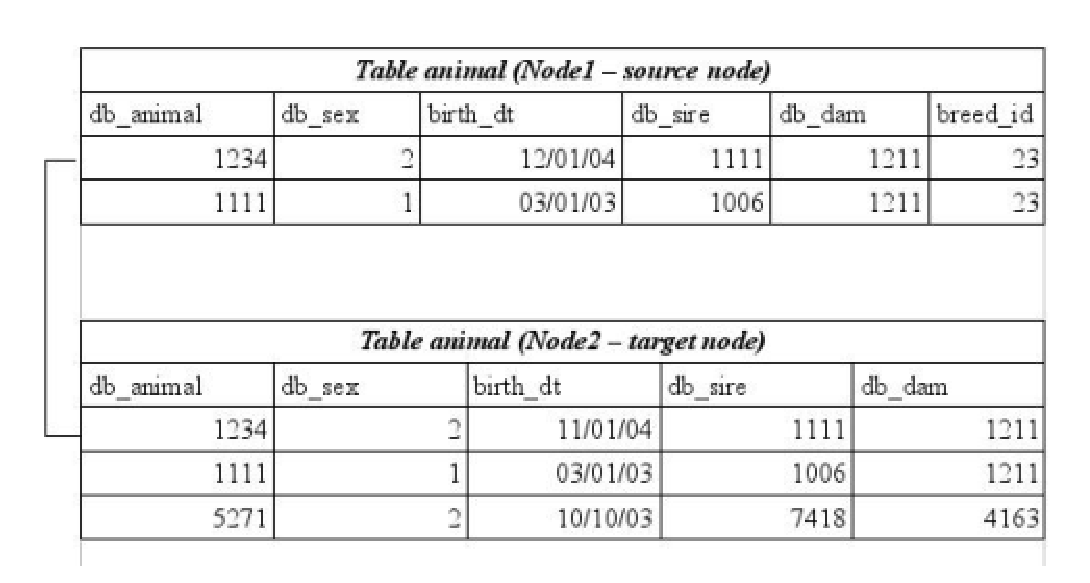
\includegraphics[%
  width=1.0\linewidth]{./synchronization/tables.eps}\end{center}

\begin{center}Information part: (1234,2,12/01/04,1111,1211)\end{center}
\end{figure}
\\
Two nodes can exchange information by setting source/target fields
of the desired data element. For consistency reasons the following
rule should apply: The source field of DE in the receiver node is
the address of the sender node and the target field of the sender
contains the receiver address . \\
This data flow, managed by setting source/target fields is regulated
by Network manager in cooperation with all nodes, thus preventing
inconsistencies in the system.\\
Also, as stated before, only owner can make representative changes
of a data element and this changes are obligatory for all other nodes.

In a generic system there will be three type of nodes:

\begin{itemize}
\item nodes that are only sources of information for the others
\item nodes that are only targets
\item nodes that are sources for some data elements and targets for other
data elements
\end{itemize}
An example of such general animal biodiversity system topology is
shown on Figure \ref{cap:General-system-topology}.%
\begin{figure}

\caption{General system topology\label{cap:General-system-topology}}

\begin{center}\includegraphics[%
  width=1.0\linewidth,
  keepaspectratio]{./synchronization/univtopology.eps}\end{center}
\end{figure}
 NODE3 is an example of the first kind, NODE4 - of the second and
NODE1 and NODE2 are examples of the third kind. In this example the
content of NODE4 will look like on Figure \ref{cap:NODE4-data-content}.
%
\begin{figure}

\caption{NODE4 data content\label{cap:NODE4-data-content}}

\begin{center}\includegraphics{./synchronization/nodedata.eps}\end{center}
\end{figure}
In the defined above terms {}``Data from NODE3'' means data owned
by NODE3 (initially loaded in NODE3). This data can be received via
NODE1 or NODE2 and the route depends on the source-target pairs. It
is possible that part of the data elements are distributed via NODE1
and part - via NODE2, but it is not possible that one data element
has NODE1 and NODE2 as sources simultaneously.


\section{Functional model}

The functional model of the synchronization process of farm animal
data is shown on Figure \ref{cap:Functional-model}. %
\begin{figure}

\caption{Functional model\label{cap:Functional-model}}

\begin{center}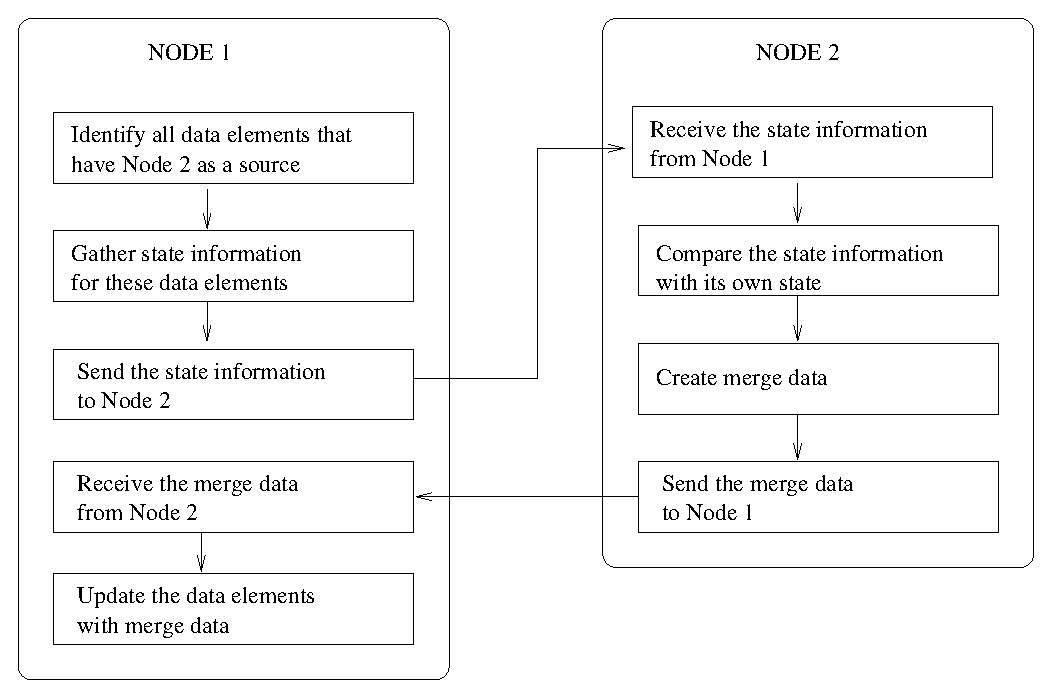
\includegraphics[%
  width=1.0\linewidth]{./synchronization/functmodel.eps}\end{center}
\end{figure}

\section{Implementation}
The implementation has to include the following steps:
\begin{itemize}
\item Setting unique node name\\
Each node has to have unique name within the APIIS-network. THis name is given by the local administrator, but has to be co-ordinated with the Network Manager. The name is set in the local '/etc/apiisrc' file.

\begin{verbatim}
[SYNCHRONISATION]
node_name = EAAP
\end{verbatim} 

\item Setting unique node ip\_address
Each node must have static ip\_address which is accessible from each node within the network. In addition port 5431 has to be open for incomming connections (this is the port where the server daemon listens). The ip\_address is also set in local '/etc/apiisrc' file

\begin{verbatim}
[SYNCHRONISATION]
node_ip = 10.1.1.126
\end{verbatim} 

\item Setting unique numbering interval
Each node in the system has to have unique record numbers and also unique animal internal numbers. The numbering range has to be obtained from from Network Manager and set in local '/etc/apiisrc' file:

\begin{verbatim}
[SYNCHRONISATION]
sequence_interval=1:100000000
\end{verbatim} 

The initialization of all sequence generators is done via the 'CreateDatabase' subroutine. It encapsulates the subroutines: 'LoadNodeData' and 'SetSequences' which are responsible for loading the local nodename and address in the database and setting the numbering interval for all sequences.
\item Setting information about the other nodes in the network
This is done via the program 'nodemanagement.pl' using the menu Settings$>$Nodes.
\item Setting information about the sources
This is done via the program 'nodemanagement.pl' using the menu Settings$>$Sources.
\item Setting information about the targets
This is done via the program 'nodemanagement.pl' using the menu Settings$>$Targets.
\end{itemize}


\chapter{XML and APIIS model}

Writing a model file as a simple text file always consumes a lot of
time and is not protected of making mistakes that can have effect
on further work with other APIIS tools. Working with a text editor
usual does not give the completely picture of a document stricture
that makes changes in the model file difficult and slow. In order
to use faster and safety way for writing and editing a model file
XML standard is implemented for describing data model structure of
APIIS. 


\section{Why XML?}

:) 


\section{Needed modules}

The names of needed modules are written in file \emph{needed\_modules}
in pdbl tree. 


\subsection{Parsing XML document}

From many existing perl parsers of XML documents are chosen two that
are standard for Perl 5.6.1 - XML::Parser and XML::Writer. Usual these
modules are installed during regular perl installation in folder named
\emph{xml}. They use stream methods of parsing that are faster and
take less memory for storage of data elements which was the reason
for their usage.

For better XML print a code, version of XML::Writer, \emph{myWriter}
is improved specially for APIIS.


\subsection{Document Type Definition (DTD) of APIIS model in XML standard }

APIIS model file is described in XML DTD format via the structure
given in the figure \ref{modeldtd} . The root element is the \emph{model}
with sub elements or children \emph{general} and \emph{table}. The
sub elements of \emph{table} are \emph{column} and \emph{TABLE. TRIGGER}
and \emph{CONSTRAINTS} are sub elements of \emph{TABLE.}

%
\begin{figure}[htbp]

\caption{The XML structure of APIIS model \label{modeldtd}}

\begin{center}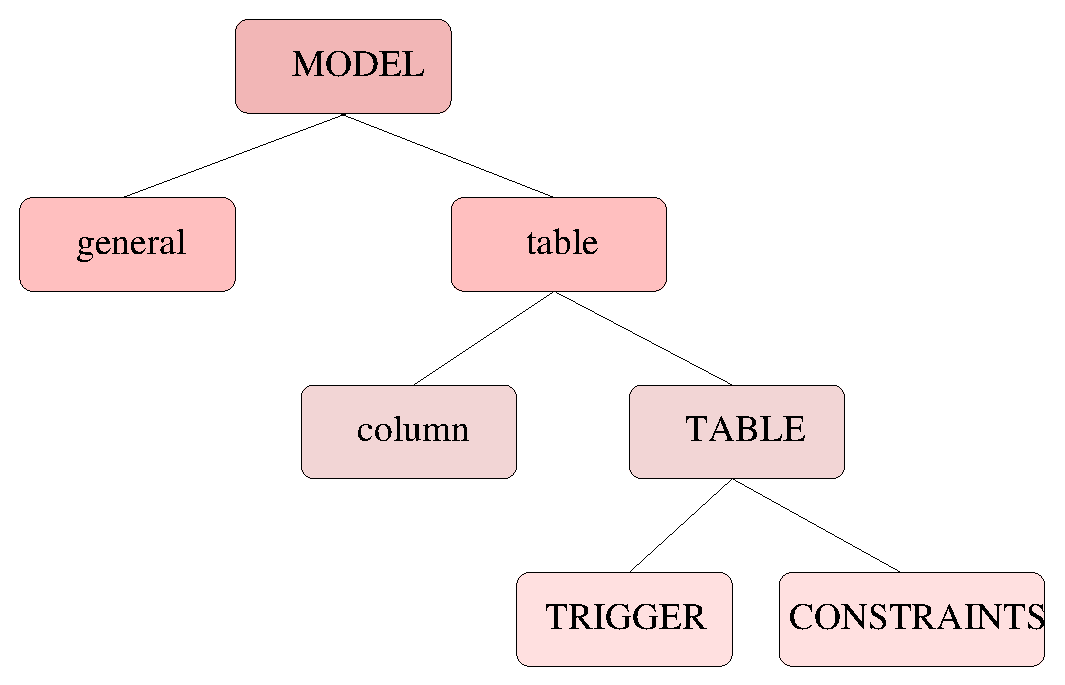
\includegraphics[%
  scale=0.4]{./XML-model/modeldtd.eps}\end{center}
\end{figure}


The DTD file on the figure \ref{DTDfile} shows the elements definitions
in APIIS model XML format as well as their attributes' lists. As attributes
are better processed by some XML editors they are preferred here.
Usage of attributes allows default values that facilitates the inserts
of model elements. It can be seen that elements marked by '+' are
these appearing more than ones in the model structure like \emph{table}
and \emph{column}.

%
\begin{table}[htbp]

\caption{DTD file of APIIS model \label{DTDfile}}

{\scriptsize <!DOCTYPE model {[}}{\scriptsize \par}

{\scriptsize <!ELEMENT model (general,table+)>}{\scriptsize \par}

{\scriptsize <!ELEMENT general EMPTY>}{\scriptsize \par}

{\scriptsize <!ATTLIST general }{\scriptsize \par}

{\scriptsize dbdriver (Pg|Oracle|CSV|InterBase|Sybase) \char`\"{}Pg\char`\"{}}{\scriptsize \par}

{\scriptsize dbname CDATA \#REQUIRED}{\scriptsize \par}

{\scriptsize dbhost CDATA \char`\"{}localhost\char`\"{}}{\scriptsize \par}

{\scriptsize dbport CDATA \char`\"{}5432\char`\"{}}{\scriptsize \par}

{\scriptsize dbuser CDATA \char`\"{}\$user\char`\"{}}{\scriptsize \par}

{\scriptsize dbpassword CDATA \char`\"{}\char`\"{}>}{\scriptsize \par}

{\scriptsize <!ELEMENT table (column+,TABLE)>}{\scriptsize \par}

{\scriptsize <!ATTLIST table}{\scriptsize \par}

{\scriptsize name CDATA \#REQUIRED>}{\scriptsize \par}

{\scriptsize <!ELEMENT column EMPTY>}{\scriptsize \par}

{\scriptsize <!ATTLIST column DATA CDATA \char`\"{}\char`\"{}}{\scriptsize \par}

{\scriptsize name CDATA \#REQUIRED}{\scriptsize \par}

{\scriptsize DATATYPE}{\scriptsize \par}

{\scriptsize (CHAR|HUGEINT|BIGINT|SMALLINT|DATE|TIME|TIMESTAMP|SMALLFLOAT|BIGFLOAT|BOOL)
\char`\"{}CHAR\char`\"{}}{\scriptsize \par}

{\scriptsize LENGTH CDATA \char`\"{}20\char`\"{}}{\scriptsize \par}

{\scriptsize DESCRIPTION CDATA \#REQUIRED}{\scriptsize \par}

{\scriptsize DEFAULT CDATA \char`\"{}\char`\"{}}{\scriptsize \par}

{\scriptsize CHECK CDATA \char`\"{}\char`\"{}}{\scriptsize \par}

{\scriptsize MODIFY CDATA \char`\"{}\char`\"{}}{\scriptsize \par}

{\scriptsize ERROR CDATA \char`\"{}\char`\"{}>}{\scriptsize \par}

{\scriptsize <!ELEMENT TABLE (TRIGGER,CONSTRAINTS)> }{\scriptsize \par}

{\scriptsize <!ELEMENT TRIGGER EMPTY>}{\scriptsize \par}

{\scriptsize <!ATTLIST TRIGGER PREINSERT CDATA \char`\"{}\char`\"{}}{\scriptsize \par}

{\scriptsize POSTINSERT CDATA \char`\"{}\char`\"{}}{\scriptsize \par}

{\scriptsize PREUPDATE CDATA \char`\"{}\char`\"{}}{\scriptsize \par}

{\scriptsize POSTUPDATE CDATA \char`\"{}\char`\"{}}{\scriptsize \par}

{\scriptsize PREDELETE CDATA \char`\"{}\char`\"{}}{\scriptsize \par}

{\scriptsize POSTDELETE CDATA \char`\"{}\char`\"{}>}{\scriptsize \par}

{\scriptsize <!ELEMENT CONSTRAINTS EMPTY>}{\scriptsize \par}

{\scriptsize <!ATTLIST CONSTRAINTS }{\scriptsize \par}

{\scriptsize PRIMARYKEY CDATA \char`\"{}\char`\"{}}{\scriptsize \par}

{\scriptsize SEQUENCE CDATA \char`\"{}\char`\"{}}{\scriptsize \par}

{\scriptsize INDEX CDATA \char`\"{}\char`\"{}> {]}>}
\end{table}



\subsection{Converting the model file to XML format}

The perl code \emph{model2xml.pl} converts the model file to XML format.
Location is in \emph{pdbl/bin}. The syntax is the next:

\emph{model2xml model\_filename xml\_filename,} where the first argument
is the model file name and second is the xml file name that is better
to have extension \emph{xml} for further work with some XML editors. 


\subsection{Extracting APIIS model file from XML document }

Extracting the mode file from xml formatted file is done by perl code
\emph{xml2model}.\emph{pl} located in \emph{pdbl/bin}. The syntax
is the next:

\emph{xml2model} \emph{xml\_filename model\_filename}, where the arguments
are with the same meaning as in 8.2.3. Here the default values of
the elements' arguments are taken automatically from DTD file. The
size of xml format file is twice less than usual model format file
because all default values are not saved.


\subsection{Editing of XML documents }

XML editors process XML documents usual in GUI environment where all
existing xml elements are accessible for editing, moving and copies.
All operations are controlled via DTD file or XML scheme. The entire
structure of the document is in tree view that can be easy processed. 

So far editor of choice is \emph{Xerlin} available in http://www.xerlin.org.
It demands Java machine to be installed. 


\section{How to use? }

The idea is using the document type definition in 'model.dtd' and
working with the program 'xerlin' to write the model file in format
of xml document. The process is facilitated via usage of libraries
of elements: columns and tables in which the main DB structure of
APIIS is implemented. 


\subsection{Creating a new model file}

Steps:

\begin{enumerate}
\item Open library apiis.xmllib from where the necessary elements could
be copied or simply 'drop and drag'.
\item Start new file with choice of DTD file model.dtd from pdbl/lib that
will be used for xml structure control and checks.
\item Insert the root element of the document - \emph{model} and first its
child - general. 
\item Take from library the main table xml equivalents
\item Insert other elements
\end{enumerate}
For creating a complete model file is recommended to start with root
element although the program offers you to choose from which element
to start.

All attributes with mandatory values (\#REQUIERED) are marked to be
inserted before next element starts. The context menus of the right
mouse button in Xerlin offer to choose among legal operations and
elements according the DTD and current content of the document. All
operations are restricted by context and logical structure in DTD
that protect the user from making mistakes. In the context menu only
legal elements are accessed and can be inserted after, before or into
a current element.

When an element is chosen its attributes are shown in right panel,
default values are there and we insert only attribute values which
are different from default ones.

The result file contains all elements of table and column types and
their attributes. The default attributes' values are not recorded
in this file if the property 'merlot.write.default-attr' has a value
'false' in preference panel. 


\subsection{Editing the model file}

To produce APIIS format model file in syntax we use in APIIS environment
is used the module \emph{xml2model.pl}. The result file is used by
other APIIS applications. In case the model file needs to be changed
in Xerlin it is reversed in xml format via module model2xml.pl. 


\subsection{Using alternative XML editors.}

In case Xerlin is not accessible another xml editor could be used. 

\begin{enumerate}
\item xemacs 
\item kate
\item kxmleditor
\end{enumerate}
If they are appropriate will be investigated.(so far they are weaker
than Xerlin) 



\chapter{Report Generator}
This is Ulf's magnificent report generator. Her only needs to add the
documentation here. 

\section{Einleitung}
Reports haben zum Ziel, Daten in einer strukturierten Form zu
visualisieren und dabei verschieden Ausgabenmedien zu
unterst�tzen. Mit dem vorliegenden Reportmodul k�nnen Daten aus
verschiedenen Quellen verarbeitet und f�r verschiedene Ausgabemedien
aufbereitet werden.

\section{Allgemeiner Aufbau eines Berichtes}

Ein Bericht besteht aus obligatorischen und nicht obligatorischen
Bereich. Jeder Bereich enth�lt eine wahlweise Anzahl von Elementen,
welche die darzustellenden Informationen enthalten. Bereiche und
Elemente werden durch Eigenschaften n�her beschrieben: 

\begin{itemize}
\item Bereich1 (Eigenschaften)
\begin{itemize}
\item Element (Eigenschaften
\item Element (Eigenschaften)
\end{itemize}
\item Bereich2 (Eigenschaften)
\begin{itemize}
\item Element ...
\end{itemize}
\end{itemize}

Aufbau, Inhalt und Struktur eines Berichtes sind in einem XML - File
definiert. Die Extension jedes Berichts-Konfigurations-Files lautet
"*.rpt " Ein Bericht kann mit einem beliebigen "XML-Editor" erstellt
werden. Die Formatvorlage dazu ist in der Datei "report.dtd"
gespeichert.

\subsection{Bereiche}

Ein Bericht kann in verschiedene Bereiche unterteilt werden. Jeder
Bereich erf�llt dabei eine bestimmte Funktion. Die Bereiche General
und Detail sind obligatorisch. GroupHeader und GroupFooter k�nnen
mehrmals definiert werden, alle anderen nur ein- oder
keinmal. Innerhalb der Bereiche k�nnen beliebig viele Elemente
platziert werden.

\begin{itemize}
\item General (obligatorisch)
  \begin{itemize}
\item GUIHeader
\item PageHeader
\item GroupHeader (mehrfach definierbar)
\item Detail (obligatorisch)
\item GroupFooter
\item PageFooter
\item GUIFooter
  \end{itemize}
\end{itemize}

\subsubsection{General}

In diesem Bereich werden allgemeine, den Bericht betreffende
Eigenschaften definiert. Er enth�lt keine Elemente.  Folgende
Eigenschaften sind g�ltig. (n�here Erl�uterungen s. Abschnitt
Eigenschaften):


\begin{itemize}
\item Name (obligatorisch)
\item DataSource (obligatorisch)
\item Width
\item CharSet
\item PageHeader
\item PageFooter
\item Border
\end{itemize}


\subsubsection{GUIHeader / GUIFooter}

Die Bereiche GUIHeader und GUIFooter werden grunds�tzlich als erster
und letzter Bereich eines Berichtes gedruckt. G�ltige Eigenschaften
sind (Erl�uterungen s. Abschnitt Eigenschaften):

\begin{itemize}
\item Name (obligatorisch)
  \begin{itemize}
  \item Height
  \item BackgroundColor
  \end{itemize}
\end{itemize}


\subsubsection{PageHeader / PageFooter}

Die Bereiche PageHeader und PageFooter werden grunds�tzlich als erster
und letzter Bereich einer Seite gedruckt. G�ltige Eigenschaften sind
(Erl�uterungen s. Abschnitt Eigenschaften):

\begin{itemize}
\item Name (obligatorisch)
\begin{itemize}
\item Height
\item BackgroundColor
\end{itemize}
\end{itemize}


\subsubsection{GroupHeader / GroupFooter}

Es besteht innerhalb eines Berichtes die M�glichkeit, Daten zu
gruppieren. Die zu gruppierende Spalte mu� im Datenstrom enthalten
sein. Die Bereiche GroupHeader / GroupFooter sind die einzigen
Bereiche, die mehrmals definiert werden k�nnen, damit die Daten nach
mehreren Informationen gruppiert werden k�nnen. G�ltige Eigenschaften
sind (Erl�uterungen s. Abschnitt Eigenschaften):

\underline{GroupHeader}
\begin{itemize}
\item Name (obligatorisch)
\begin{itemize}
\item Height
\item GroupFooterName (obligatorisch)
\item Background Color
\item KeepTogether
\item Group 	(obligatorisch)
\item GroupOn
\item Sort
\end{itemize}
\end{itemize}

\underline{GroupFooter}
\begin{itemize}
\item Name 	(obligatorisch)
\begin{itemize}
\item Height
\item BackgroundColor
\end{itemize}
\end{itemize}

\subsubsection{Detail}

Der Bereich "Detail" ist die kleinste Einheit eines Berichtes. Hier
werden die einzelnen Datens�tze angezeigt. G�ltige Eigenschaften sind
(Erl�uterungen s. Abschnitt Eigenschaften): 

\begin{itemize}
\item Name 	(obligatorisch)
  \begin{itemize}
  \item Height
  \item BackgroundColor
  \end{itemize}
\end{itemize}

\section{Elemente}
Innerhalb der Bereiche k�nnen Elemente platziert werden, die wiederum
Eigenschaften besitzen.  Die kursiv gedruckten Eigenschaften sind noch
nicht implementiert. 

\subsection{Text}

Text-Elemente sind fix und zeigen nur die vorher definierten Werte
an. Typische Anwendungen sind �berschriften, Labels u.s.w. G�ltige
Eigenschaften sind (Erl�uterungen s. Abschnitt Eigenschaften): 
 
\begin{multicols}{2}
\begin{itemize}
\item Name  	(obligatorisch)
\begin{itemize}
\item Content 	(obligatorisch)
\end{itemize}

\underline{Position}

\item Position
\item Left
\item Top
\item Height
\item Width
\item Clip
\item Column	(obligatorisch)
\item Row	(obligatorisch)

\underline{ Font}

\item FontFamily
\item FontSize
\item FontStyle
\item FontWeight
\item FontVariant
\item Font

\underline{Color}

\item BackgroundColor
\item Color
\item BackgroundImage
\item BackgroundRepeat
\item BackgroundAttachment
\item BackgroundPosition
\item Visibility

\underline{Letter}

\item WordSpacing
\item LetterSpacing
\item TextDecoration
\item VerticalAlign
\item TextTransform
\item TextAlign
\item TextIndent
\item LineHeight

\underline{Box}

\item MarginTop
\item MarginRight
\item MarginBottom
\item MarginLeft
\item Margin
\item PaddingTop
\item PaddingRight
\item PaddingBottom
\item Paddingleft
\item Padding

\underline{Border}

\item BorderTopWidth
\item BorderRightWidth
\item BorderLeftWidth
\item BorderBottomWidth
\item BorderWidth
\item BorderStyle
\item BorderColor
\item BorderTop
\item BorderRight
\item BorderLeft
\item BorderBottom
\item Border
\item BlockWidth
\item BlockHeight
\item BlockFloat
\item Clear
\item Display
\item WhiteSpace
\item ListStyleType
\item ListStyleImage
\item ListStylePosition
\item ListStyle
\end{itemize}

\end{multicols}

\subsubsection{Hidden}
Dieses
Element dient dazu, Werte zwischenzuspeichern. Diese Daten werden
nicht angezeigt. G�ltige Eigenschaften sind (Erl�uterungen
s. Abschnitt Eigenschaften):

\begin{itemize}
\item Name  	(obligatorisch)
  \begin{itemize}
  \item Content 	(obligatorisch)
  \end{itemize}
\end{itemize}
  

\subsubsection{Data}
Data-Elemente
stellen Inhalte dar, die erst nach dem Start eines Reports verf�gbar
sind. Au�erdem ist es mit diesen Feldern m�glich, Inhalte
anderer Elemente anzuzeigen. G�ltige Eigenschaften sind
(Erl�uterungen s. Abschnitt Eigenschaften):

\begin{multicols}{2}
\begin{itemize}
\item Name  	(obligatorisch)
\begin{itemize}
\item Content 	(obligatorisch)
\item DecimalPlaces
\item Format
\item RunningSums
\end{itemize}

\underline{Position}

\item Position
\item Left
\item Top
\item Height
\item Width
\item Clip
\item Column	(obligatorisch)
\item Row	(obligatorisch)

\underline{Font}

\item FontFamily
\item FontSize
\item FontStyle
\item FontWeight
\item FontVariant
\item Font

\underline{Color}

\item BackgroundColor
\item Color
\item BackgroundImage
\item BackgroundRepeat
\item BackgroundAttachment
\item BackgroundPosition
\item Visibility

\underline{Letter}

\item WordSpacing
\item LetterSpacing
\item TextDecoration
\item VerticalAlign
\item TextTransform
\item TextAlign
\item TextIndent
\item LineHeight

\underline{Box}

\item MarginTop
\item MarginRight
\item MarginBottom
\item MarginLeft
\item Margin
\item PaddingTop
\item PaddingRight
\item PaddingBottom
\item Paddingleft
\item Padding

\underline{Border}

\item BorderTopWidth
\item BorderRightWidth
\item BorderLeftWidth
\item BorderBottomWidth
\item BorderWidth
\item BorderStyle
\item BorderColor
\item BorderTop
\item BorderRight
\item BorderLeft
\item BorderBottom
\item Border
\item BlockWidth
\item BlockHeight
\item BlockFloat
\item Clear
\item Display
\item WhiteSpace
\item ListStyleType
\item ListStyleImage
\item ListStylePosition
\item ListStyle
\end{itemize}

\end{multicols}

\subsubsection{Lines}
Lines-Elemente stellen verschiedene Arten Linien dar. G�ltige
Eigenschaften sind (Erl�uterungen s. Abschnitt Eigenschaften): 

\begin{multicols}{2}
\underline{Allgemein}
\begin{itemize}
\item Name  	(obligatorisch)
\begin{itemize}
\item Content 	(obligatorisch)
\item ForegroundColor
\item LineType
\item LineWidth
\end{itemize}

\underline{Position}

\item Left
\item Top
\item Column	(obligatorisch)
\item Row	(obligatorisch)

\underline{Box}

\item MarginTop
\item MarginRight
\item MarginBottom
\item MarginLeft
\item Margin
\item PaddingTop
\item PaddingRight
\item PaddingBottom
\item Paddingleft
\item Padding

\underline{Border}

\item BorderTopWidth
\item BorderRightWidth
\item BorderLeftWidth
\item BorderBottomWidth
\item BorderWidth
\item BorderStyle
\item BorderColor
\item BorderTop
\item BorderRight
\item BorderLeft
\item BorderBottom
\item Border
\end{itemize}
\end{multicols}

\subsubsection{PageBreak}
PageBreak-Elemente stellen verschiedene Arten Linien dar. G�ltige
Eigenschaften sind (Erl�uterungen s. Abschnitt
Eigenschaften). PageBreak-Elemente sind noch nicht implementiert: 

\underline{Allgemein}
\begin{itemize}
\item Name  	(obligatorisch)
\begin{itemize}
\item Left
\item Top
\end{itemize}
\end{itemize}

\subsubsection{SubGUI}
Mit diesem Element k�nnen Unterberichte eingebettet
werden. Unterberichte haben die Endung "*.srpt" und sind separat zu
definieren. G�ltige Eigenschaften sind (Erl�uterungen s. Abschnitt
Eigenschaften): 

\begin{multicols}{2}
\underline{Allgemein}
\begin{itemize}
\item Name  	(obligatorisch)
\begin{itemize}
\item GUISource 	(obligatorisch)
\item Visible

\underline{Position}

\item Left
\item Top
\item Height
\item Width
\item Column	(obligatorisch)
\item Row	(obligatorisch)
\end{itemize}
\end{itemize}
\end{multicols}


\subsubsection{Images}
Images-Elemente stellen Bilder dar. G�ltige Eigenschaften sind
(Erl�uterungen s. Abschnitt Eigenschaften): 

\begin{multicols}{2}
\underline{Allgemein}
\begin{itemize}
\item Name  	(obligatorisch)
\begin{itemize}
\item ImageSourde	(obligatorisch)
\item Visible

\underline{Position}

\item Left
\item Top
\item Height
\item Width
\item Column	(obligatorisch)
\item Row	(obligatorisch) 

\underline{Box}

\item MarginTop
\item MarginRight
\item MarginBottom
\item MarginLeft
\item Margin
\item PaddingTop
\item PaddingRight
\item PaddingBottom
\item Paddingleft
\item Padding

\underline{Border}

\item BorderTopWidth
\item BorderRightWidth
\item BorderLeftWidth
\item BorderBottomWidth
\item BorderWidth
\item BorderStyle
\item BorderColor
\item BorderTop
\item BorderRight
\item BorderLeft
\item BorderBottom
\item Border
\end{itemize}
\end{itemize}
\end{multicols}

\subsection{Eigenschaften}

\subsubsection{Positionsangaben}
\newcommand{\tab}{\hspace{5mm}}

\begin{longtable}{|p{0.639in}|p{2.893in}|p{0.968in}|}
\hline
% ROW 1
{\centering \textbf{Einstellung}} & 
{\centering \textbf{Beschreibung}} & 
{\centering \textbf{Beispiel}}\\
\hline
% ROW 2
{\raggedright position} & 
{\raggedright Hier\"{u}ber wird ein Element positioniert. Die Einstellung \textit{static} ist 
die Defaulteinstellung, die nicht explizit angegeben werden muss. 
Das Element, das statisch positioniert worden ist, kann nicht 
in der Position bewegt werden. \"{U}ber \textit{absolute} ist das Element 
unabh\"{a}ngig von anderen Elementen positioniert. re\textit{lative} setzt 
das Element relativ zu einem anderen Element.} & 
{\raggedright position:relative}\\
\hline
% ROW 3
{\raggedright left} & 
{\raggedright Diese Angabe legt die Position in der x-Achse fest.} & 
{\raggedright left:100px;}\\
\hline
% ROW 4
{\raggedright top} & 
{\raggedright Diese Angabe legt die Position in der y-Achse fest.} & 
{\raggedright top:100px;}\\
\hline
% ROW 5
{\raggedright width} & 
{\raggedright Diese Angabe gibt die Breite des Elements an.} & 
{\raggedright width:50px;}\\
\hline
% ROW 6
{\raggedright height} & 
{\raggedright Diese Angabe gibt die Breite des Elements an.} & 
{\raggedright height:50px;}\\
\hline
% ROW 7
{\raggedright clip} & 
{\raggedright Hier\"{u}ber k\"{o}nnen Sie von einem Element einen kleinen Bereich 
darstellen. Dazu wird ein Rechteck eingestellt, das an eine bestimmte 
Position innerhalb des Taginhalts gesetzt wird. Allgemein:  \linebreak
clip: rect (\texttt{<}top\texttt{>} \texttt{<}right\texttt{>} \texttt{<}bottom\texttt{>} 
\texttt{<}left\texttt{>}) \linebreak
\textit{rect} legt ein Rechteck innerhalb des Elements an, das an 
die Positionen \texttt{<}top\texttt{>} \texttt{<}right\texttt{>} \texttt{<}bottom\texttt{>} 
\texttt{<}left\texttt{>} (Angabe in Pixel!) gesetzt wird.} & 
{\raggedright clip:rect (10px 50px 20px 0px) ;}\\
\hline
% ROW 8
{\raggedright visibility} & 
{\raggedright Hier\"{u}ber stellen Sie die Sichtbarkeit ein. \textit{Visibility:visible} ist 
die Standarteinstellung, die das Element sichtbar macht. Mit 
\textit{visibility:hidden} wird das Element versteckt.} & 
{\raggedright visibility:hidden}\\
\hline
\end{longtable}

{\underline {Font-Angaben}}

\begin{longtable}{|p{0.639in}|p{2.893in}|p{0.968in}|}
\hline
% ROW 1
{\centering \textbf{Einstellung}} & 
{\centering \textbf{Beschreibung}} & 
{\centering \textbf{Beispiel}}\\
\hline
% ROW 2
{\raggedright font-family} & 
{\raggedright Dies gibt eine Liste von Schriftfamilien an, die verwendet werden 
k\"{o}nnen. Ist die erste nicht vorhanden, wird die zweite angegebene 
Fontfamilie verwendet. Die einzelnen Angaben sind durch ein Komma 
zu trennen.} & 
{\raggedright font-family: gill, helvetica, sans-serif;}\\
\hline
% ROW 3
{\raggedright font-style} & 
{\raggedright Diese angaben kann drei Werte \textit{normal, italic, oblique} annehmen. 
Der Wert \textit{normal} gibt den normalen, ausgew\"{a}hlten Font an. 
\textit{italic} setzt den Font kursiv und \textit{oblique} wird verwendet 
wenn der Schrifttyp nicht als kursiver Typ (also als \textit{italic}- 
Wert) verf\"{u}gbar ist.} & 
{\raggedright font-style: italic;}\\
\hline
% ROW 4
{\raggedright font-variant} & 
{\raggedright Diese Angabe legt fest, ob der Font \textit{normal} oder \textit{small-caps} 
dargestellt wird. In der Einstellung \textit{small-caps} werden alle 
kleinen Buchstaben in der gleichen Gr\"{o}{�}e wie Gro{�}buchstaben 
dargestellt.} & 
{\raggedright font-variant: small-caps;}\\
\hline
% ROW 5
{\raggedright font-weight} & 
{\raggedright Diese Angabe legt fest wie, wie fett ein Font dargestellt werden 
soll. Die m\"{o}glichen Werte sind: \textit{normal, bold, bolder, lighter, 
100, 200,300, 400, 500, 600, 700, 800, 900}.Die Einstellung \textit{font-weight}: 
normal ist identisch mit \textit{font-weight: 400. font-weight: 700} 
ist identisch mit \textit{font-weight:bold}.} & 
{\raggedright font-weight: 800}\\
\hline
% ROW 6
{\raggedright font-size} & 
{\raggedright Gibt die Gr\"{o}{�}e des Fonts in der Punktgr\"{o}{�}e (pt) an.} & 
{\raggedright font-size: 12pt;}\\
\hline
% ROW 7
{\raggedright font} & 
{\raggedright Dies ist eine Abk\"{u}rzung und umfasst mehrere Angaben zusammen: 
\textit{font-style, font-variant, font-weight, font-size, line-height 
und font-family}} & 
{\raggedright font: 13pt sans-serif small-caps;}\\
\hline
\end{longtable}

{\underline {COLOR- und BACKGROUND-Angaben}}

\begin{longtable}{|p{0.722in}|p{2.979in}|p{0.798in}|}
\hline
% ROW 1
{\centering \textbf{Einstellung}} & 
{\centering \textbf{Beschreibung}} & 
{\centering \textbf{Beispiel}}\\
\hline
% ROW 2
{\raggedright color} & 
{\raggedright Dies bestimmt die Vordergrundfarbe. Sie k\"{o}nnen entweder die 
vordefinierten Farbnamenverwenden, den hexadezimalen Code einer 
jeden Farbe oder die RGB- Werte.} & 
{\raggedright color:red}\\
\hline
% ROW 3
{\raggedright background-color} & 
{\raggedright Dies bestimmt die Hintergrundfarbe. Sie k\"{o}nnen entweder die 
vordefinierten Farbnamen verwenden, den hexadezimalen Code einer 
jeden Farbe oder die RGB- Werte.} & 
{\raggedright backgroundcolor: black}\\
\hline
% ROW 4
{\raggedright background-image} & 
{\raggedright Hier\"{u}ber k\"{o}nnen Sie ein Hintergrundbild f\"{u}r das Element 
laden.} & 
{\raggedright backgroundimage: url (blume.jpg);}\\
\hline
% ROW 5
{\raggedright background-repeat} & 
{\raggedright Hier\"{u}ber legen Sie fest, wie das geladene Hintergrundbild 
zu behandeln ist. \textit{repeat} ist die Default-Einstellung, die 
das Bild horizontal und vertikal kachelt. Mit \textit{repeat-x} wird 
das Bild horizontal gekachelt. \textit{repeat-y} kachelt das Bild 
vertikal \textit{und no-repeat} kachelt das Hintergrundbild nicht.} & 
{\raggedright background-repeat: repeat-y;}\\
\hline
% ROW 6
{\raggedright background-attachment} & 
{\raggedright Diese Einstellung legt fest, ob der Hintergrund gescrollt (\textit{scroll}) 
wird, wenn der Internet-Surfer die Bildlaufleisten bet\"{a}tigt, 
oder ob der Hintergrund fest stehen bleiben soll (\textit{fixed}).} & 
{\raggedright background-attachment: fixed;}\\
\hline
% ROW 7
{\raggedright background-position} & 
{\raggedright Hier\"{u}ber k\"{o}nnen Sie die Position des Hintergrunds innerhalb 
des Elements festlegen. Die Standartangaben erfolgen in Prozent, 
aber auch feste Werte sind m\"{o}glich.} & 
{\raggedright background-position:50\% \linebreak
50\%}\\
\hline
% ROW 8
{\raggedright background} & 
{\raggedright Dies ist analog zu \textit{font} eine Zusammenfassung von mehreren 
Eigenschaften: \textit{background-color, background-image, background-repeat, 
bachground-attachment} und \textit{background-position}} & 
{\raggedright background: url (pfeile.jpg) aqua repeat-x fixed;}\\
\hline
\end{longtable}

{\underline {Textangaben}}

\begin{longtable}{|p{0.702in}|p{2.912in}|p{0.886in}|}
\hline
% ROW 1
{\centering \textbf{Einstellung}} & 
{\centering \textbf{Beschreibung}} & 
{\centering \textbf{Beispiel}}\\
\hline
% ROW 2
{\raggedright word-spacing} & 
{\raggedright Diese Eigenschaften legen den Raum zwischen den W\"{o}rtern fest.} & 
{\raggedright word-spacing: 0.4cm;}\\
\hline
% ROW 3
{\raggedright letter-spacing} & 
{\raggedright Diese Eigenschaft legt den Raum zwischen zwei Zeichen fest.} & 
{\raggedright Letter-spacing:0.lem;}\\
\hline
% ROW 4
{\raggedright text-decoration} & 
{\raggedright Diese Eigenschaft gibt an, ob der Text dekoriert, d.h. unterstrichen 
(\textit{underline}), durchgestrichen (\textit{line-through}) oder blinkend 
(\textit{blink}) dargestellt werden soll.} & 
{\raggedright Text-decoration: underline;}\\
\hline
% ROW 5
{\raggedright vertical-align} & 
{\raggedright Dies legt die vertikale Ausrichtung fest. Die m\"{o}glichen Einstellungen 
sind \textit{baseline, middle, sub, super, text-top, text-bottom, 
top, bottom}.} & 
{\raggedright Vertical-align: sub;}\\
\hline
% ROW 6
{\raggedright text-transform} & 
{\raggedright Diese Eigenschaft gibt an, wie die Buchstaben ausgegeben werden 
sollen. Die m\"{o}glichen Einstellungen sind: \textit{capitalize} (der 
erste Buchstabe eines jeden Wortes wird gro{�} geschrieben), 
\textit{uppercase} (alle Buchstaben werden gro{�} geschrieben), \textit{lowcrase} (alle 
Buchstaben werden klein geschrieben) und \textit{none} (keine Bestimmung 
\"{u}ber die Gro{�}- und Kleinschreibung der Buchstaben).} & 
{\raggedright text-transform: uppercase;}\\
\hline
% ROW 7
{\raggedright text-align} & 
{\raggedright Diese Eigenschaft gibt die horizontale Ausrichtung eines Textes 
an. Die m\"{o}glichen Werte sind: \textit{left, right, center, justify.}} & 
{\raggedright text-align: center;}\\
\hline
% ROW 8
{\raggedright text indent} & 
{\raggedright Diese Eigenschaft gibt den Einzug eines Textes an.} & 
{\raggedright text-indent: 0.5cm;}\\
\hline
% ROW 9
{\raggedright line-height} & 
{\raggedright Hier wird der vertikale Abstand zwischen zwei Grundlinien als 
Zeilenh\"{o}he gesetzt.} & 
{\raggedright Line-height.1.2; font-size:10pt}\\
\hline
\end{longtable}

{\underline {Blockdaten}}

\begin{longtable}{|p{0.809in}|p{2.787in}|p{0.904in}|}
\hline
% ROW 1
{\centering \textbf{Einstellung}} & 
{\centering \textbf{Beschreibung}} & 
{\centering \textbf{Beispiel}}\\
\hline
% ROW 2
{\raggedright margin-top} & 
{\raggedright Setzt den Abstand zwischen einen oberen Rahmen eines Blocks 
und dem n\"{a}chsten Element.} & 
{\raggedright margin-top:lem}\\
\hline
% ROW 3
{\raggedright margin-right} & 
{\raggedright Setzt den Abstand zwischen einem rechten Rahmen eines Blocks 
und dem n\"{a}chsten Element.} & 
{\raggedright margin-right:lem}\\
\hline
% ROW 4
{\raggedright margin- bottom} & 
{\raggedright Setzt den Abstand zwischen einem unteren Rahmen eines Blocks 
und dem n\"{a}chsten Element.} & 
{\raggedright margin-bottom:lem}\\
\hline
% ROW 5
{\raggedright margin-left} & 
{\raggedright Setzt den Abstand zwischen einem linken Rahmen eines Blocks 
und dem n\"{a}chsten Element.} & 
{\raggedright margin-left:10em}\\
\hline
% ROW 6
{\raggedright margin} & 
{\raggedright Dies ist eine Zusammenfassung der vier Eigenschaften \textit{margin-top, 
margin-right, margin-bottom, margin-left.} Die Parameter werden 
in dieser Reihenfolge nacheinander angegeben} & 
{\raggedright margin:1em 1em 1em 1em }\\
\hline
% ROW 7
{\raggedright padding-top} & 
{\raggedright Setzt den Abstand zwischen dem oberen Rand eines Rahmens eines 
Blocks und dessen Inhalt.} & 
{\raggedright padding-top:10px}\\
\hline
% ROW 8
{\raggedright padding-right} & 
{\raggedright Setzt den Abstand zwischen dem rechten Rand eines Rahmens eines 
Blocks und dessen Inhalt.} & 
{\raggedright padding-right:10px}\\
\hline
% ROW 9
{\raggedright padding-bottom} & 
{\raggedright Setzt den Abstand zwischen dem unteren Rand eines Rahmens eines 
Blocks und dessen Inhalt.} & 
{\raggedright padding-bottom:10px}\\
\hline
% ROW 10
{\raggedright padding-left} & 
{\raggedright Setzt den linken Abstand zwischen dem linken Rand eines Rahmens 
eines Blocks und dessen Inhalt.} & 
{\raggedright padding-left:10px}\\
\hline
% ROW 11
{\raggedright padding } & 
{\raggedright Dies ist eine Zusammenfassung der vier Eigenschaften \textit{padding-top, 
padding-right, padding-bottom, padding-left,} Die Parameter werden 
in dieser Reihenfolge nacheinander eingegeben.} & 
{\raggedright padding:10px 10px 10px 10px}\\
\hline
% ROW 12
{\raggedright border-top-width} & 
{\raggedright Setzt die Breite der oberen Rahmenlinie.} & 
{\raggedright border-top-width:2pt}\\
\hline
% ROW 13
{\raggedright border-right-widht} & 
{\raggedright Setzt die Breite der rechten Rahmenlinie.} & 
{\raggedright border-right-width:2pt}\\
\hline
% ROW 14
{\raggedright border-bottom-width} & 
{\raggedright Setzt die Breite der unteren Rahmenlinie.} & 
{\raggedright Bordr.bottom-width:2pt}\\
\hline
% ROW 15
{\raggedright border-left-width} & 
{\raggedright Setzt die Breite der linken Rahmenlinie.} & 
{\raggedright border-left-width:2pt}\\
\hline
% ROW 16
{\raggedright border-width} & 
{\raggedright Dies ist eine Zusammenfassung der vier Eigenschaften \textit{border-top-width, 
border-right-width, border-bottom-width, border-left-width}. Die 
Parameter werden in dieser Reihenfolge nacheinander angegeben.} & 
{\raggedright border-width:2pt 2pt 2pt 2pt }\\
\hline
% ROW 17
{\raggedright border-style} & 
{\raggedright Setzt den Stil des Rahmens. Die m\"{o}glichen Einstellungen sind 
\textit{none, solid, double, inset, outset, groove, ridge, dooted, 
dashed}.} & 
{\raggedright border-style:solid}\\
\hline
% ROW 18
{\raggedright border-color} & 
{\raggedright Setzt die Farbe des Rahmens} & 
{\raggedright border-color:blue}\\
\hline
% ROW 19
{\raggedright border-top} & 
{\raggedright Das ist die Zusammenfassung der Eigenschaften \textit{border-top-width, 
border-style} und \textit{border-color}. Die Parameter werden in dieser 
Reihenfolge nacheinander angegeben.} & 
{\raggedright border-top:2pt solid blue}\\
\hline
% ROW 20
{\raggedright border-right} & 
{\raggedright Dies ist eine Zusammenfassung der Eigenschaften \textit{border-right-width, 
border-style} und \textit{border-color.} Die Parameter werden in dieser 
Reihenfolge nacheinander dargestellt.} & 
{\raggedright border-right:2pt solid blue}\\
\hline
% ROW 21
{\raggedright border-bottom} & 
{\raggedright Dies ist eine Zusammenfassung der Eigenschaften border-bottom-width, 
border-style und \textit{border-color}. Die Parameter werden in dieser 
Reihenfolge nacheinander angegeben.} & 
{\raggedright border-bottom:2pt solid blue}\\
\hline
% ROW 22
{\raggedright border left} & 
{\raggedright Dies ist eine Zusammenfassung der Eigenschaften \textit{border-left-width, 
border-style} und \textit{border-color}. Die Parameter werden in dieser 
Reihenfolge nacheinander angegeben.} & 
{\raggedright border-left.pt solid blue}\\
\hline
% ROW 23
{\raggedright border} & 
{\raggedright Dies ist eine Zusammenfassung der Eigenschaften \textit{border-width, 
border-style} und \textit{border-color}.} & 
{\raggedright border:2pt solid blue}\\
\hline
% ROW 24
{\raggedright width } & 
{\raggedright Legt die breite des Blocks fest.} & 
{\raggedright width: 50px}\\
\hline
% ROW 25
{\raggedright height} & 
{\raggedright Legt die H\"{o}he eines Blocks fest.} & 
{\raggedright height: 50px}\\
\hline
% ROW 26
{\raggedright float} & 
{\raggedright Legt die Ausrichtung des Blocks durch \textit{none, left} oder \textit{right} 
fest.} & 
{\raggedright foat: right}\\
\hline
% ROW 27
{\raggedright clear} & 
{\raggedright Legt fest bei welcher Seite kein Text umflie{�}en darf. Die 
m\"{o}glichen Einstellungen sind\textit{: none, left, right} oder \textit{both.}} & 
{\raggedright Clear:both}\\
\hline
% ROW 28
{\raggedright display} & 
{\raggedright  Diese Eigenschaft legt fest, wie das Element gezeichnet werden 
soll. Die m\"{o}glichen Werte sind: \textit{block, inline, list-item, 
none. block} \"{o}ffnet eine neue Zeichenfl\"{a}che, relativ zum vorhergehenden 
Element. \textit{inline} \"{o}ffnet das Element innerhalb der aktuellen 
Zeile. \textit{list-item} arbeitet wie \textit{block}, wobei das Element 
aber als Element innerhalb eines Blocks angesehen wird. \textit{none} unterdr\"{u}ckt 
das Zeichen des Elements.} & 
{\raggedright display: block}\\
\hline
% ROW 29
{\raggedright white-space} & 
{\raggedright Diese Eigenschaft legt fest, wie die so genannten White-Space-Zeichen 
(d.h. Leerzeichen und Tabs) behandelt werden sollen. Die Einstellung 
\textit{normal} behandelt die Zeichen, wie sie sind w\"{a}hrend die 
Einstellung \textit{pre} die Zeichen wie das HTML-Tag \texttt{<}PRE\texttt{>} behandelt} & 
{\raggedright white-space:normal}\\
\hline
% ROW 30
{\raggedright list-style-type} & 
{\raggedright Das legt das Aussehen der Aufz\"{a}hlungszeichen fest. Die m\"{o}glichen 
Einstellungen sind: \textit{disc, circle, square, decimal, lower-roman, 
upper-roman. lower-alpha, upper-alpha} oder \textit{none.}} & 
{\raggedright list-style-type: disc}\\
\hline
% ROW 31
{\raggedright list-style-image} & 
{\raggedright Dies legt eine graphik als Aufz\"{a}hlungszeichen fest.} & 
{\raggedright list-style-image: url (blume.jpg)}\\
\hline
% ROW 32
{\raggedright list-style-position} & 
{\raggedright Gibt an, ob das Aufz\"{a}hlungselement einger\"{u}ckt (\textit{inside}) 
oder ausger\"{u}ckt (\textit{outside}) werden soll.} & 
{\raggedright {\underline {?}}}\\
\hline
% ROW 33
{\raggedright List-style} & 
{\raggedright Dies fasst die Eigenschaften \textit{list-style-type} und \textit{list-style-position} 
zusammen.} & 
{\raggedright list-style: disc outside}\\
\hline
\end{longtable}

\section{ Beispiel}

Auf einer Leistungspr\"{u}fung wurden die Gewichte verschiedener 
Rassen ermittelt. Die Gewichte sollen drei Gruppen zugeordnet 
werden. Darzustellen sind die Nummern der Tiere, sowie deren 
Gewichte innerhalb der Rasse und der Gewichtsgruppe. Weiterhin 
ist f\"{u}r jede Gruppe und f\"{u}r jede Rasse die Anzahl der Tiere 
sowie das Gruppenmittel anzugeben. Am Ende des Berichtes soll 
das Gruppenmittel der beiden Rassen dargestellt werden.

\subsection{ Erstellen einer Abfrage oder einer Funktion}

Bevor ein Bericht als Layout erstellt wird, m\"{u}ssen die Daten 
zusammengestellt werden. Das kann \"{u}ber ein SQL-Statement erfolgen 
oder \"{u}ber eine Funktion, falls das Daten zusammenstellen umfangreicher 
ist. Es ist wichtig, dass die Funktion bzw. das SQL-Statement 
getestet sind und die erwarteten Daten liefern.

\subsection{Entwurf eines Layouts.}

Bevor mit dem Entwurf eines Reports begonnen wird, ist die Struktur 
und das Aussehen zu konzipieren. Dazu wird aufgezeichnet, welche 
Informationen auf dem Bericht dargestellt werden sollen und wie 
diese formatiert sind.

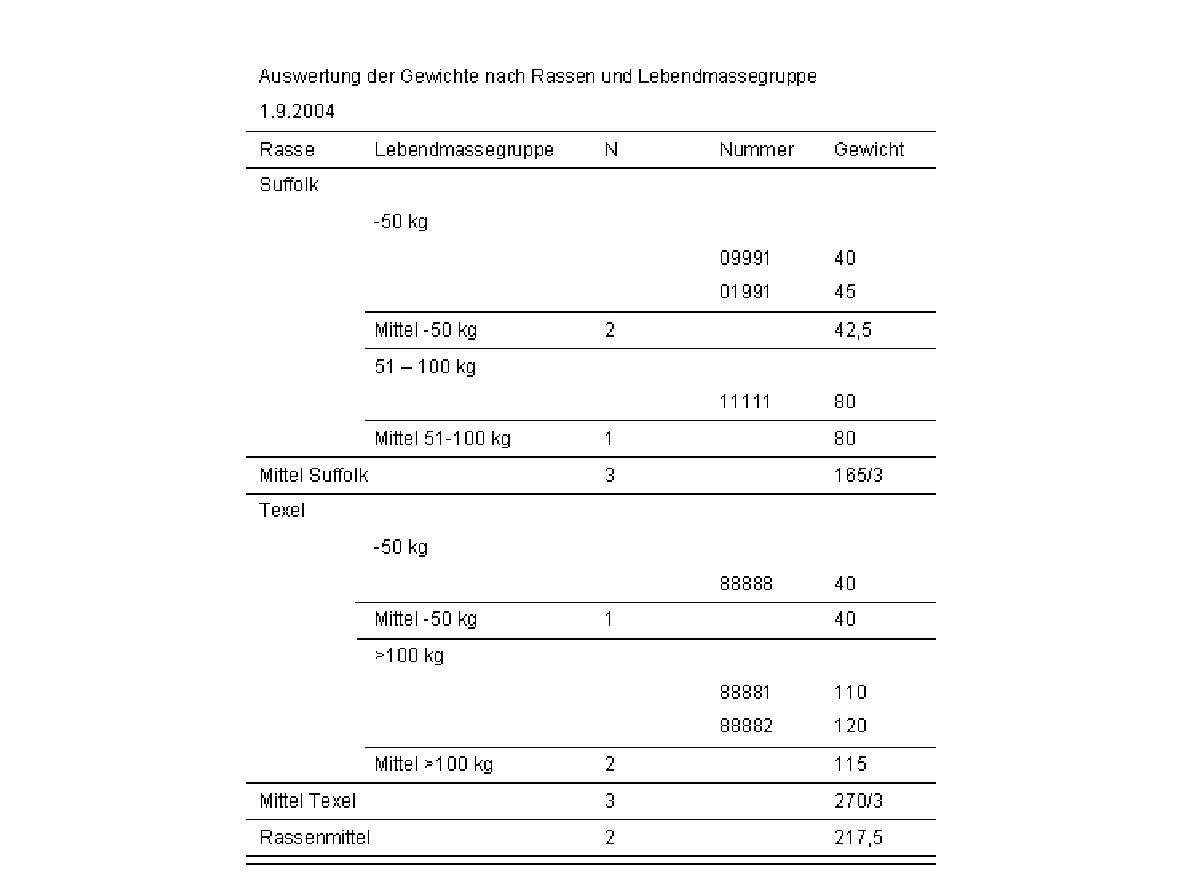
\includegraphics[width=160mm]{./report-gen/pic3.eps}

\subsection{Gliederung des Reports in Bereiche}


Im n\"{a}chsten Schritt wird der Bericht in einzelne Bereiche gegliedert. 

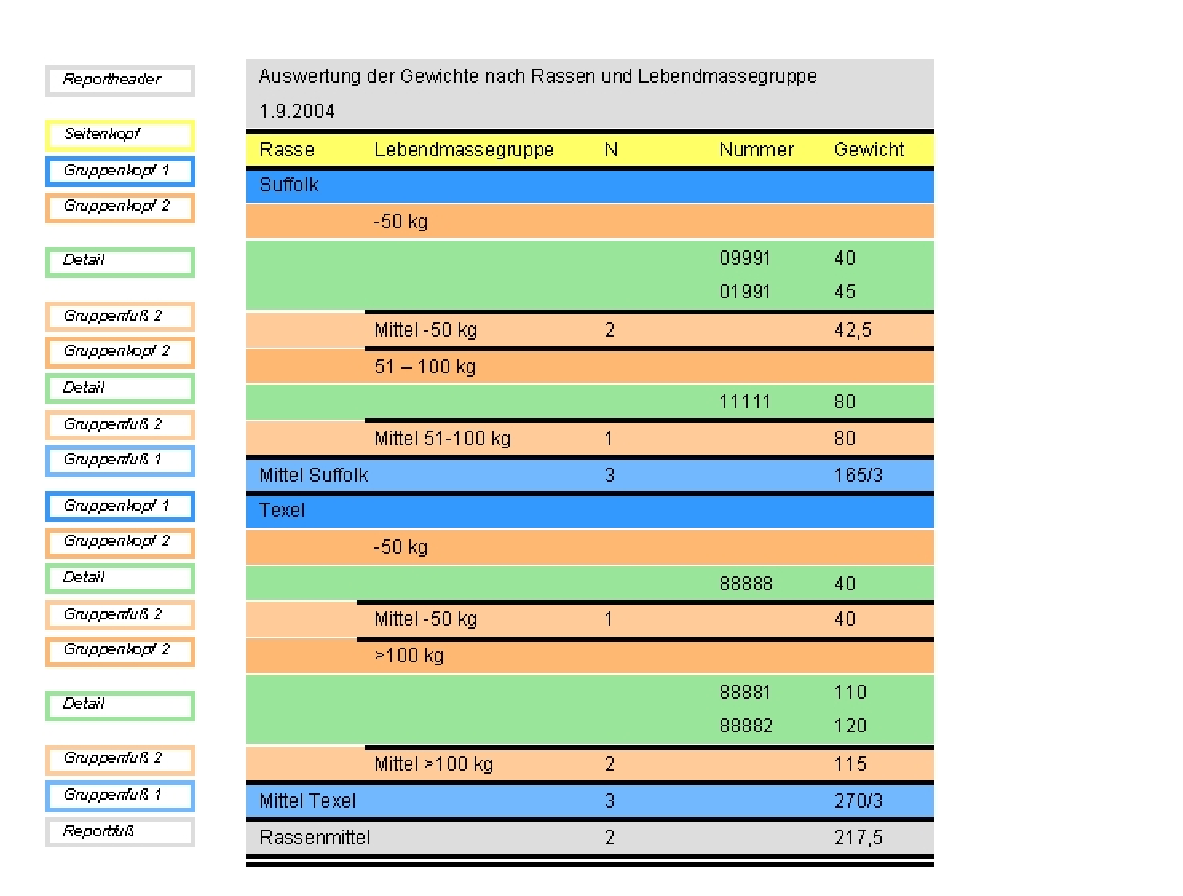
\includegraphics[width=160mm]{./report-gen/pic2}
\includegraphics[width=160mm]{./report-gen/pic4}
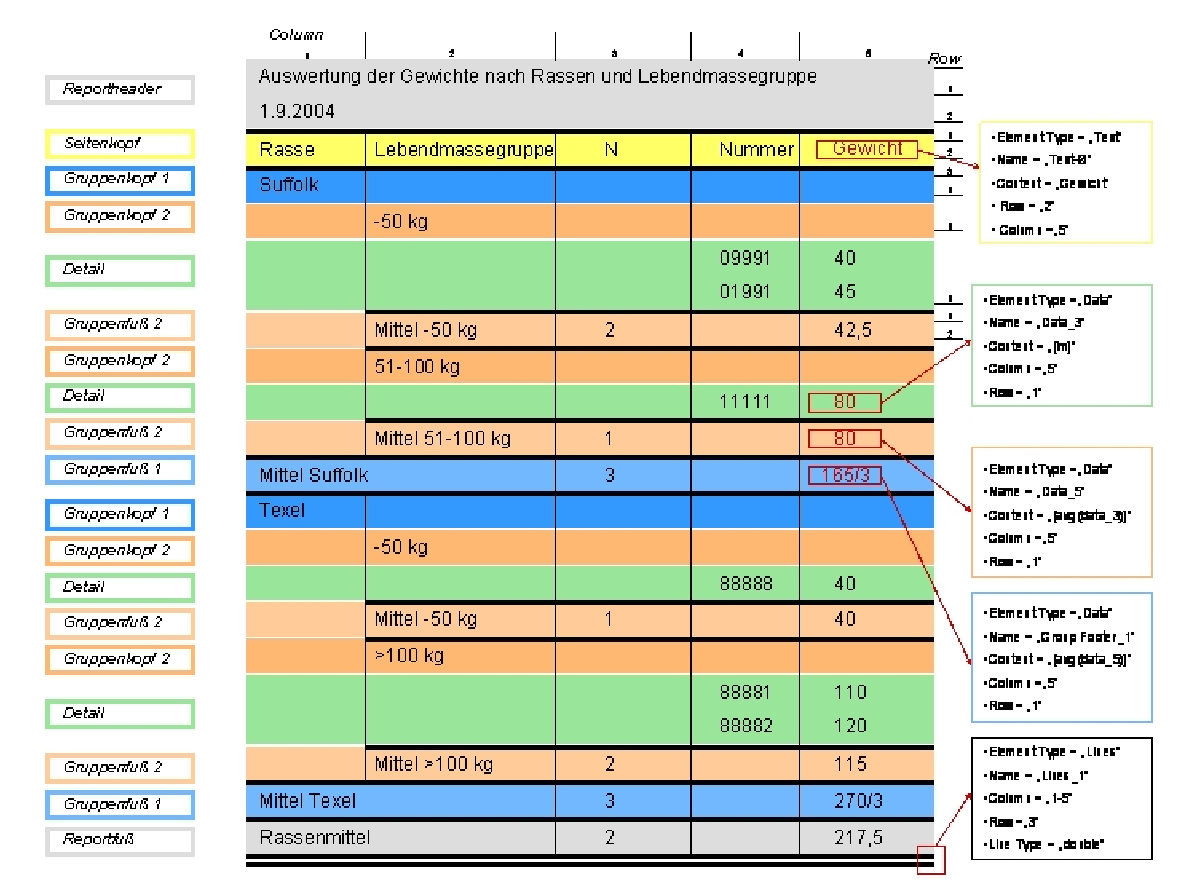
\includegraphics[width=160mm]{./report-gen/pic1}

Im n\"{a}chsten Schritt wird jedes einzelne Element des Berichtes 
als Objekt gekennzeichnet. Dabei werden f\"{u}r jedes Objekt folgende 
Attribute gesetzt:

\begin{itemize}
\item Art des Objektes (ElementType)
\item Bezeichnung (Name)
\item Inhalt (Content)
\end{itemize}

Im Beispiel werden die Elementypen ,,Linien``, ,,Text ,, und ,,Data`` 
vergeben. W\"{a}hrend Textobjekte nur Zeichen darstellen k\"{o}nnen, 
werden ,,Data`` -- Objekte verwendet, wenn die Datenquelle andere 
Objekte sind, statistische Funktionen angewendet werden sollenoder 
die Daten aus einem SQL -- Statement oder einer Funktion kommen. 

\tab Die Bezeichnung der Objekte mu{�} eindeutig sein.

In Data- Objekten m\"{u}ssen Verweise in der allgemeinen Form 


\begin{center}
Funktion ([Verweisziel])


\end{center}
angegeben werden.

Im n\"{a}chsten Schritt werden Spaltenhilfslinien \"{u}ber den Bericht 
gelegt. Damit wird gekennzeichnet, welche Informationen in einer 
Spalte stehen sollen. Es ist dabei grunds\"{a}tzlich m\"{o}glich, 
dass Objekte \"{u}ber mehr als eine Spalte gehen.

F\"{u}r alle Objekte mu{�} in der Eigenschaft ,,Column`` die Spalte 
eingetragen werden. F\"{u}r Objekte, die mehr als eine Spalte einnehmen, 
ist der bereich anzugeben: 2-4

Weiterhin ist die Eigenschaft ``Row`` zu setzen. Die Nummerierung 
erfolgt innerhalb eines Bereiches.

Als letztes wird das Layout der Objekte definiert - die Textgr\"{o}{�}e, 
Schrift, Schriftgrad, u.s.w.

Sind diese Vorbereitungen abgeschlossen ist das Konfigurationsfile 
zu erstellen. Es ist ein XML -- File, dass einen beliebigen Namen, 
aber die fixe Endung ,,.rpt `` besitzen darf

Die vollst\"{a}ndige Listung stellt Abb. dar.

Zum Erstellen und Editieren des Kofigurationsfiles kann ein beliebiger 
XML -- Editor verwendet werden. Die g\"{u}ltigen Elemente und Attribute 
eines Berichtes sind in der ,,report.ata`` -- Document -- Typ -- 
Definition beschrieben.

\tab MS java -- jar Xerlin\dots 

\tab \tab \"{O}ffnen der Document -- Typ -- Definition

\tab  \tab Erstellen des Konfigurationsfile durch Hinzuf\"{u}gen der entsprechenden 

Elemente

\section{Aufruf eines Berichtes}

\subsection{Kommandozeile als ASCII}

\tab Report -- o\tab ascii\tab parameter

Bsp.\tab Report -- o\tab ascii\tab vclass = `41'

Der Bericht wird auf der Console angegeben.

{\underline {{\Large DataSource}}}

Ausgangspunkt f\"{u}r die Darstellung eines Berichtes ist ein Datenstrom, 
der alle notwendigen Basisinformationen enth\"{a}lt. Dabei werden 
Daten aus drei verschiedenen Quellen entgegengenommen

\begin{enumerate}
\item SQL -- Statement
\item Perl -- Funktionen
\item ASCII -- File
\item Dateneingabe in einem Form
\end{enumerate}

Bsp.: 

\tab DataSource = (Select * from tabelle)

\tab DataSource = \$ form name. object

\tab DataSource = @\{function()\}

\tab Datasource = filename

Zur Abgrenzung der drei Varianten m\"{u}ssen SQL -- Statements in 
einer runden Klammer eingeschlossen sein.

Zur \"{U}bergabe von Parametern k\"{o}nnen in einem SQL -- Statement 
geschweifte Klammern verwendet werden. Innerhalb der Klammern 
ist ein Verweis auf ein Objekt eines g\"{u}ltigen Forms notwendig

\tab \tab z.B.: (Select * from codes where class ='\{\$formname.objekt\}')

Bei der Bereitstellung der Daten \"{u}ber eine Funktion ist der 
Funktionsname anzugeben, gefolgt von einer \"{o}ffnenden und einem 
schlie{�}enden runden Klammer. Innerhalb der Klammern k\"{o}nnen 
mit Komma getrennt Parameter \"{u}bergeben werden

\tab = funktion ( \$formname.objekt, ,irgendwas' )

Liegen die darzustellenden Daten in einem ASCII -- File , so ist 
der vollst\"{a}ndige Pfadname anzugeben.

Steht ein Dollarzeichen am Anfang, wird angenommen, dass der 
einzuf\"{u}gende Text in einem Formular eingegeben wurde.

In diesem Fall mu{�} die Eingabe nach der Aufl\"{o}sung ein SQL 
-- Statement (mit Klammer am Anfange und Ende), eine Funktion 
(Klammern am Ende) oder ein Filenamen ergeben.

{\underline {Funktionen}}

Auf alle Daten in Data -- Objekten (und nur dort) k\"{o}nnen Funktionen 
angewendet werden. Mit Funktionen k\"{o}nnen Daten aggregiert oder 
ver\"{a}ndert werden.

Funktionen k\"{o}nnen sich nur auf Daten innerhalb des Reports 
beziehen. Es wird zwischen Funktionen mit und ohne Parameter 
unterschieden.

Funktionen ohne Parameter 

\begin{itemize}
\item date ( ) - gibt das aktuelle Datum wieder
\item user ( ) - gibt den aktuellen user zur\"{u}ck
\item vnd ( ) - gibt eine Zufallszahl zur\"{u}ck
\end{itemize}

Funktionen mit Parameter:

Ein Parameter kann eine Zahl sein oder ein Verweis auf den Inhalt 
eines anderen Data -- Objects.

\tab allg. Form:\tab \tab funktion\tab ([verweis])

\tab Funktionen:

\begin{itemize}
\item avg ( ) -  Mittelwert
\item std ( ) - Standartabweichung
\item  min ( ) - Minimum
\item max ( ) - Maximum
\item first ( ) - erster Wert
\item last ( ) - letzter Wert
\end{itemize}








\printindex
\end{document}
